% =============================================================================
%  LUẬN VĂN THẠC SĨ
%  Đề tài: Tối ưu phân bổ tài nguyên sử dụng Học tăng cường sâu
%          trong mạng STAR-RIS hỗ trợ RSMA
%  Tác giả: Nguyễn Duy Thanh
%  Trường: Đại học Giao thông vận tải TP. Hồ Chí Minh (UTH)
%  Compiler: XeLaTeX  +  BibTeX (IEEEtran.bst)
% =============================================================================
\documentclass{uth-thesis}

% --- Thông tin luận văn -----------------------------------------------------
\thesisuniversity{Trường Đại học Giao thông vận tải TP. Hồ Chí Minh}
\thesisfaculty{Viện Đào tạo Sau đại học}
\thesisauthor{Nguyễn Duy Thanh}
\thesistitle{Tối ưu phân bổ tài nguyên sử dụng học tăng cường sâu trong mạng STAR-RIS hỗ trợ RSMA}
\thesisadvisor{1. TS. Trần Thiên Thanh \\ 2. TS. Ngô Hoàng Tú}
\thesismajor{Khoa học máy tính}
\thesissubmajor{Khoa học máy tính}
\thesismajorcode{2480101831}
\thesisyear{2026}
\thesiscity{TP. Hồ Chí Minh}

% =============================================================================
%  TỐI ƯU COMPILE (TUỲ CHỌN)
% =============================================================================
% Khi sửa nội dung và muốn compile NHANH (< 10s), bỏ comment 1 trong các dòng:
% \includeonly{chapters/04_chuong_3}     % chỉ compile Ch3
% \includeonly{chapters/05_chuong_4}     % chỉ compile Ch4
% \includeonly{chapters/02_chuong_1,chapters/03_chuong_2}  % chỉ Ch1+Ch2
%
% Khi build BẢN ĐẦY ĐỦ để nộp: comment lại các dòng \includeonly ở trên (như hiện tại).
% =============================================================================

\begin{document}

% =============================================================================
%  PHẦN TRƯỚC (đánh số La Mã cho front matter)
% =============================================================================
\pagenumbering{roman}
\setcounter{page}{1}

% 1. Trang bìa chính
\makecoverpage

% 2. Trang bìa phụ
\makeinnercoverpage

% 3. Lời cam đoan, lời cảm ơn, tóm tắt, mục lục, danh mục
% =============================================================================
%  Front matter: Lời cam đoan, Lời cảm ơn, Tóm tắt, Mục lục, Danh mục
% =============================================================================

% --------- LỜI CAM ĐOAN -----------------------------------------------------
\clearpage
\thispagestyle{empty}
\begin{center}
{\fontsize{14}{17}\bfseries\MakeUppercase Lời cam đoan\par}
\end{center}
\vspace{1cm}

\hspace{1.27cm}Tôi xin cam đoan đây là công trình nghiên cứu của riêng tôi. Các
số liệu, kết quả thực nghiệm và kết luận nêu trong Luận văn là trung thực và
chưa từng được công bố trong bất kỳ công trình nào khác. Toàn bộ mã nguồn,
dữ liệu huấn luyện, các hình ảnh và bảng biểu trình bày trong Luận văn đều
do tôi tự xây dựng, ngoại trừ những phần đã trích dẫn nguồn rõ ràng trong
mục Tài liệu tham khảo theo chuẩn IEEE.

\vspace{0.5cm}
\hspace{1.27cm}Tôi xin chịu trách nhiệm về đề tài nghiên cứu của mình.

\vspace{2cm}
\begin{flushright}
\begin{minipage}{0.45\textwidth}
\centering
TP. Hồ Chí Minh, ngày \ldots\ tháng \ldots\ năm 2026\\[0.3cm]
Tác giả Luận văn\\[2.5cm]
\textbf{Nguyễn Duy Thanh}
\end{minipage}
\end{flushright}

% --------- LỜI CẢM ƠN -------------------------------------------------------
\clearpage
\thispagestyle{empty}
\begin{center}
{\fontsize{14}{17}\bfseries\MakeUppercase Lời cảm ơn\par}
\end{center}
\vspace{1cm}

\hspace{1.27cm}Để hoàn thành Luận văn Thạc sĩ này, tôi đã nhận được sự giúp đỡ
và hỗ trợ quý báu từ nhiều cá nhân và tổ chức. Tôi xin được bày tỏ lòng biết ơn
sâu sắc đến:

\vspace{0.3cm}
\hspace{1.27cm}\textbf{TS. Trần Thiên Thanh} và \textbf{TS. Ngô Hoàng Tú},
hai người hướng dẫn khoa học, đã tận tình chỉ bảo, định hướng nghiên cứu
và động viên tôi trong suốt quá trình thực hiện đề tài. Những góp ý quý
báu của hai Thầy về cả mặt lý thuyết và triển khai mô phỏng đã giúp Luận
văn có được kết quả như hiện tại.

\vspace{0.3cm}
\hspace{1.27cm}\textbf{Quý Thầy, Cô Viện Đào tạo Sau đại học và Khoa Công
nghệ Thông tin, Trường Đại học Giao thông vận tải TP. Hồ Chí Minh} đã
trang bị cho tôi nền tảng kiến thức vững chắc về khoa học máy tính, trí
tuệ nhân tạo và xử lý dữ liệu, là cơ sở thiết yếu để thực hiện công trình
này.

\vspace{0.3cm}
\hspace{1.27cm}\textbf{Cộng đồng nghiên cứu mã nguồn mở} (PyTorch, NumPy,
Matplotlib, draw.io) đã cung cấp các công cụ giúp việc cài đặt, huấn luyện
và trực quan hóa kết quả thực nghiệm trở nên thuận tiện và đáng tin cậy.

\vspace{0.3cm}
\hspace{1.27cm}\textbf{Gia đình và bạn bè} đã luôn ở bên động viên, chia sẻ và
hỗ trợ tôi cả về vật chất lẫn tinh thần trong suốt thời gian học tập và
nghiên cứu.

\vspace{0.5cm}
\hspace{1.27cm}Mặc dù đã có nhiều cố gắng, song do giới hạn về thời gian và
kinh nghiệm, Luận văn không tránh khỏi những thiếu sót. Tôi rất mong nhận
được ý kiến đóng góp của quý Thầy/Cô và bạn đọc để Luận văn được hoàn thiện
hơn.

\vspace{0.5cm}
\hspace{1.27cm}Xin trân trọng cảm ơn!

\vspace{1.5cm}
\begin{flushright}
\begin{minipage}{0.45\textwidth}
\centering
TP. Hồ Chí Minh, ngày \ldots\ tháng \ldots\ năm 2026\\[0.3cm]
Tác giả Luận văn\\[2.5cm]
\textbf{Nguyễn Duy Thanh}
\end{minipage}
\end{flushright}

% --------- MỤC LỤC ----------------------------------------------------------
\clearpage
\thispagestyle{empty}
\renewcommand{\contentsname}{\hfill MỤC LỤC \hfill}
\tableofcontents

% --------- DANH MỤC TỪ VIẾT TẮT ---------------------------------------------
\clearpage
\thispagestyle{empty}
\begin{center}
{\fontsize{14}{17}\bfseries\MakeUppercase Danh mục các ký hiệu, các chữ viết tắt\par}
\end{center}
\vspace{0.4cm}

\noindent\textbf{1. Các ký hiệu toán học}\par
\vspace{0.2cm}

\renewcommand{\arraystretch}{1.2}
\setlength{\tabcolsep}{4pt}
\begin{longtable}{p{3.5cm} p{11cm}}
\toprule
\textbf{Ký hiệu} & \textbf{Ý nghĩa} \\
\midrule
\endhead
$N$ & Số phần tử của STAR-RIS \\
$K$ & Tổng số người dùng (UE) trong hệ thống \\
$K_R, K_T$ & Số UE trong vùng phản xạ R và vùng truyền qua T \\
$M$ & Số anten của trạm gốc (BS) \\
$h_{d,k}$ & Kênh truyền trực tiếp từ BS đến UE thứ $k$ \\
$\mathbf{G}$ & Vector kênh truyền từ BS đến STAR-RIS, $\mathbf{G} \in \mathbb{C}^{N \times 1}$ \\
$\mathbf{h}_{r,k}^X$ & Vector kênh từ STAR-RIS đến UE thứ $k$, vùng $X \in \{R, T\}$ \\
$h_{eff,k}$ & Kênh hiệu dụng SISO tương đương BS--UE thứ $k$ \\
$\Phi_n^X$ & Hệ số phản xạ/truyền qua của phần tử thứ $n$, $X \in \{R, T\}$ \\
$\boldsymbol{\Phi}_X$ & Ma trận pha dịch STAR-RIS vùng $X$, dạng đường chéo \\
$\beta_n^R, \beta_n^T$ & Hệ số phân chia năng lượng phản xạ/truyền qua, $\in [0,1]$ \\
$\theta_n^R, \theta_n^T$ & Pha phản xạ/truyền qua của phần tử thứ $n$, $\in [0, 2\pi)$ \\
$\sqrt{\beta_n^X}$ & Biên độ phức của hệ số STAR-RIS \\
$x$ & Tín hiệu phát hợp nhất tại BS \\
$y_k$ & Tín hiệu thu tại UE thứ $k$ \\
$s_c, s_k$ & Luồng chung và luồng riêng (mã hóa) của UE thứ $k$ \\
$W_k, W_k^c, W_k^p$ & Thông điệp gốc, phần chung, phần riêng của UE thứ $k$ \\
$P_c, P_k$ & Công suất phát dành cho luồng chung và luồng riêng UE thứ $k$ \\
$P_{\max}$ & Công suất phát tối đa của BS \\
$c_k$ & Tỷ lệ phân chia luồng chung cho UE thứ $k$, $\sum_k c_k = 1$ \\
$\sigma^2$ & Công suất tạp âm Gauss phức tại UE \\
$\gamma_{c,k}, \gamma_{p,k}$ & SINR luồng chung và luồng riêng tại UE thứ $k$ \\
$R_{c,k}, R_{p,k}$ & Tốc độ luồng chung khả thi và luồng riêng tại UE thứ $k$ \\
$R_c$ & Tốc độ luồng chung của toàn hệ thống, $R_c = \min_k R_{c,k}$ \\
$R_k$ & Tổng tốc độ của UE thứ $k$, $R_k = c_k R_c + R_{p,k}$ \\
$R_{sum}$ & Tổng tốc độ toàn hệ thống, $R_{sum} = \sum_k R_k$ \\
$R_{\min}$ & Yêu cầu QoS tối thiểu cho từng UE \\
$\alpha_d, \alpha_G, \alpha_r$ & Số mũ suy hao đường truyền cho từng loại kênh \\
$d_0, \mathrm{PL}_0$ & Khoảng cách tham chiếu và suy hao tham chiếu \\
$\mathcal{S}, \mathcal{A}, \mathcal{R}$ & Không gian trạng thái, hành động, phần thưởng (MDP) \\
$s_t, a_t, r_t$ & Trạng thái, hành động, phần thưởng tại bước thời gian $t$ \\
$o_i, a_i$ & Quan sát cục bộ và hành động của tác tử thứ $i$ \\
$\mu_i, Q_i$ & Mạng Actor và Critic của tác tử thứ $i$ \\
$\theta_{\mu_i}, \phi_i$ & Tham số trọng số mạng Actor và Critic \\
$\gamma$ & Hệ số chiết khấu của MDP, $\gamma \in [0,1)$ \\
$\tau$ & Hệ số cập nhật mềm cho mạng mục tiêu \\
$\lambda_t$ & Hệ số phạt Lagrangian thích nghi tại bước $t$ \\
$\Delta\phi_n^X$ & Phần dư pha (residual) đầu ra của tác tử pha \\
$\mathcal{N}_t^{\text{OU}}$ & Nhiễu khám phá Ornstein--Uhlenbeck \\
$|\mathcal{D}|$ & Kích thước bộ đệm phát lại (replay buffer) \\
$\mathds{1}[\cdot]$ & Hàm chỉ thị (indicator function) \\
\bottomrule
\end{longtable}

\vspace{0.4cm}
\noindent\textbf{2. Các chữ viết tắt}\par
\vspace{0.2cm}

\renewcommand{\arraystretch}{1.2}
\setlength{\tabcolsep}{4pt}
\begin{longtable}{p{2cm} p{7cm} p{5.5cm}}
\toprule
\textbf{Viết tắt} & \textbf{Tiếng Anh} & \textbf{Tiếng Việt} \\
\midrule
\endhead
6G   & Sixth Generation                       & Thế hệ thứ sáu \\
AI   & Artificial Intelligence                & Trí tuệ nhân tạo \\
BCD  & Block Coordinate Descent               & Hạ dần khối tọa độ \\
BS   & Base Station                           & Trạm gốc \\
CSI  & Channel State Information              & Thông tin trạng thái kênh \\
CTDE & Centralised Training, Decentralised Execution & Huấn luyện tập trung, thực thi phân tán \\
DDPG & Deep Deterministic Policy Gradient     & Gradient chính sách tất định sâu \\
DL   & Deep Learning                          & Học sâu \\
DRL  & Deep Reinforcement Learning            & Học tăng cường sâu \\
DQN  & Deep Q-Network                         & Mạng Q sâu \\
ES   & Energy Splitting                       & Chia tách năng lượng \\
ISAC & Integrated Sensing and Communication   & Cảm biến và truyền thông tích hợp \\
LOS  & Line of Sight                          & Đường truyền thẳng \\
MA   & Multiple Access                        & Đa truy nhập \\
MADDPG & Multi-Agent DDPG                     & DDPG đa tác tử \\
MARL & Multi-Agent Reinforcement Learning     & Học tăng cường đa tác tử \\
MDP  & Markov Decision Process                & Quá trình ra quyết định Markov \\
MIMO & Multiple-Input Multiple-Output         & Nhiều ngõ vào nhiều ngõ ra \\
MLP  & Multi-Layer Perceptron                 & Mạng nơ-ron đa lớp \\
MS   & Mode Switching                         & Chuyển đổi chế độ \\
NLOS & Non-Line-of-Sight                      & Không có đường truyền thẳng \\
NN   & Neural Network                         & Mạng nơ-ron \\
NOMA & Non-Orthogonal Multiple Access         & Đa truy nhập không trực giao \\
OFDMA & Orthogonal Frequency-Division MA      & Đa truy nhập phân chia theo tần số trực giao \\
OMA  & Orthogonal Multiple Access             & Đa truy nhập trực giao \\
OU   & Ornstein--Uhlenbeck                    & Nhiễu Ornstein--Uhlenbeck \\
PPO  & Proximal Policy Optimisation           & Tối ưu hóa chính sách lân cận \\
QoS  & Quality of Service                     & Chất lượng dịch vụ \\
ReLU & Rectified Linear Unit                  & Đơn vị tuyến tính chỉnh lưu \\
RF   & Radio Frequency                        & Tần số vô tuyến \\
RIS  & Reconfigurable Intelligent Surface     & Bề mặt phản xạ thông minh \\
RL   & Reinforcement Learning                 & Học tăng cường \\
RSMA & Rate-Splitting Multiple Access         & Đa truy nhập theo phân tách tốc độ \\
SDMA & Space-Division Multiple Access         & Đa truy nhập phân chia theo không gian \\
SIC  & Successive Interference Cancellation   & Khử nhiễu liên tiếp \\
SINR & Signal-to-Interference-plus-Noise Ratio & Tỷ số tín hiệu trên nhiễu cộng tạp âm \\
SISO & Single-Input Single-Output             & Một ngõ vào một ngõ ra \\
STAR-RIS & Simultaneously Transmitting And Reflecting RIS & RIS truyền-phản xạ đồng thời \\
SWIPT & Simultaneous Wireless Information and Power Transfer & Truyền tin và điện đồng thời \\
TD3  & Twin Delayed DDPG                      & DDPG sinh đôi trì hoãn \\
TS   & Time Switching                         & Chuyển đổi thời gian \\
UAV  & Unmanned Aerial Vehicle                & Phương tiện bay không người lái \\
UE   & User Equipment                         & Thiết bị người dùng \\
URLLC & Ultra-Reliable Low-Latency Comms.     & Truyền thông siêu tin cậy độ trễ thấp \\
\bottomrule
\end{longtable}

% --------- DANH MỤC BẢNG ----------------------------------------------------
\clearpage
\thispagestyle{empty}
\renewcommand{\listtablename}{\hfill DANH MỤC CÁC BẢNG \hfill}
\listoftables

% --------- DANH MỤC HÌNH ----------------------------------------------------
\clearpage
\thispagestyle{empty}
\renewcommand{\listfigurename}{\hfill DANH MỤC CÁC HÌNH ẢNH \hfill}
\listoffigures


% =============================================================================
%  NỘI DUNG CHÍNH (đánh số Ả-rập từ Mở đầu)
% =============================================================================
\clearpage
\pagenumbering{arabic}
\setcounter{page}{1}
\pagestyle{fancy}

% Mở đầu
% =============================================================================
%  MỞ ĐẦU (3-5 trang)
% =============================================================================
\chapter*{MỞ ĐẦU}
\addcontentsline{toc}{chapter}{MỞ ĐẦU}
\markboth{MỞ ĐẦU}{}

\section*{1. Tính cấp thiết của đề tài}
\addcontentsline{toc}{section}{1. Tính cấp thiết của đề tài}

Mạng thông tin di động thế hệ thứ sáu (6G) được kỳ vọng sẽ vượt xa các thế
hệ trước về thông lượng (lên tới $1$~Tbps), độ trễ siêu thấp (dưới
$0{,}1$~ms) và mật độ kết nối khổng lồ ($10^7$ thiết bị/km$^2$)
\cite{saad2020vision6g}, \cite{tataria20216g}. Để đáp ứng các yêu cầu khắt khe đó,
nhiều công nghệ then chốt được nghiên cứu, trong đó hai hướng nổi bật là
Đa truy nhập theo phân tách tốc độ (Rate-Splitting Multiple Access
RSMA) và Bề mặt phản xạ thông minh có khả năng truyền-phản xạ đồng thời
(Simultaneously Transmitting And Reflecting Reconfigurable Intelligent
Surface, STAR-RIS) \cite{mao2022rsma}, \cite{liu2021starris}, \cite{mu2022simultaneously}.

RSMA cho phép trạm gốc phân tách thông điệp của mỗi người dùng thành một
phần chung (common) và một phần riêng (private), sau đó truyền
đồng thời qua cùng tài nguyên thời gian-tần số. Tại phía thu, người dùng
giải mã luồng chung trước, áp dụng khử nhiễu liên tiếp (SIC) và sau đó giải
mã luồng riêng. Cách thiết kế này tạo nên khả năng quản lý nhiễu mềm dẻo
hơn so với các kỹ thuật trực giao (OMA) và không trực giao truyền thống
(NOMA), đặc biệt là trong điều kiện thông tin trạng thái kênh không hoàn
hảo \cite{mao2018rsma}, \cite{mao2022rsma}.

STAR-RIS là sự mở rộng của RIS truyền thống, gồm $N$ phần tử thụ động có thể
đồng thời điều chỉnh pha cả tín hiệu phản xạ và tín hiệu truyền qua
mặt phẳng RIS. Đặc tính này biến vùng phủ sóng từ nửa không gian
$180^\circ$ thành toàn không gian $360^\circ$, mở ra khả năng phục vụ
người dùng ở hai phía của bề mặt thông minh \cite{liu2021starris}, \cite{mu2022simultaneously}.

Tuy nhiên, khi tích hợp RSMA và STAR-RIS, bài toán phân bổ tài nguyên
trở nên cực kỳ phức tạp: ta phải đồng thời tối ưu hóa (i) công suất phát
giữa luồng chung và các luồng riêng, (ii) tỷ lệ phân chia luồng chung cho
từng người dùng, (iii) biên độ và pha của mỗi phần tử STAR-RIS ở cả hai
chế độ phản xạ và truyền qua. Bài toán này có tính phi lồi cao do các
hàm SINR phụ phi tuyến vào biến công suất và vào tích vô hướng phức của
vector pha. Các phương pháp tối ưu truyền thống như hạ dần khối tọa độ
(BCD), nới lỏng nửa xác định (SDR) hoặc tối ưu xen kẽ (AO) tuy có thể
cho lời giải gần tối ưu nhưng đòi hỏi chi phí tính toán lớn, không phù
hợp cho triển khai thời gian thực trong môi trường kênh biến thiên nhanh
\cite{wu2020smart}.

Học tăng cường sâu (DRL), và đặc biệt là phiên bản đa tác tử MADDPG
cung cấp một con đường khác: thay vì giải tường minh bài toán tối ưu, tác tử
học chính sách phân bổ tài nguyên trực tiếp từ tương tác với môi trường
\cite{sutton2018reinforcement}, \cite{lillicrap2016continuous}, \cite{lowe2017multi}.
Sau khi huấn luyện, suy luận chỉ cần một lần chạy tiến (forward pass) của
mạng nơ-ron, có độ phức tạp gần như hằng số, lý tưởng cho yêu cầu thời
gian thực của 6G \cite{noman2026drl6g}, \cite{hieu2021optimal}. Vì các lý do trên,
việc nghiên cứu ứng dụng MADDPG để tối ưu phân bổ tài nguyên trong
mạng STAR-RIS hỗ trợ RSMA mang ý nghĩa khoa học và thực tiễn rõ rệt.

\section*{2. Mục tiêu nghiên cứu}
\addcontentsline{toc}{section}{2. Mục tiêu nghiên cứu}

\noindent\textbf{Mục tiêu tổng quát:} Xây dựng và đánh giá một khuôn khổ
học tăng cường sâu đa tác tử cho bài toán tối ưu phân bổ tài nguyên đường
xuống trong mạng STAR-RIS hỗ trợ RSMA, sao cho tối đa hóa tổng tốc độ hệ
thống đồng thời tối ưu cân bằng giữa thông lượng và mức đáp ứng chất lượng
dịch vụ (QoS) của từng người dùng thông qua một hàm mục tiêu thay thế
(surrogate) dạng phạt/Lagrangian của ràng buộc QoS, tương ứng với ràng buộc
kỳ vọng $\mathbb{E}[R_k] \geq R_{\min}$.

\noindent\textbf{Mục tiêu cụ thể:}
\begin{enumerate}[label=(\arabic*),leftmargin=*]
\item Xây dựng mô hình hệ thống đầy đủ: kênh truyền (trực tiếp, gián tiếp
qua STAR-RIS, suy hao đường truyền log-distance, pha-đinh Rayleigh),
mô hình tín hiệu RSMA, và bài toán tối ưu phân bổ tài nguyên (P0) với
đầy đủ các ràng buộc về công suất, bảo toàn năng lượng STAR-RIS, phân
chia luồng chung và QoS.
\item Đề xuất khuôn khổ MADDPG với ba tác tử chuyên dụng (BS Power, STAR-RIS
Reflection, STAR-RIS Transmission) cùng hai cải tiến: (i) tham số hóa
pha residual dựa trên nghiệm phân tích bậc một và (ii) hàm phần thưởng
dạng Lagrangian với các hệ số phạt $\lambda_k$ riêng cho từng người dùng,
được cập nhật bằng phương pháp gradient đối ngẫu có phép chiếu
(projected dual gradient) trên khe hở ràng buộc có dấu
$c_k = R_{\min} - R_k$, để cân bằng tốc độ tổng và QoS.
\item Cài đặt mô phỏng và đánh giá toàn diện hiệu năng so với các baseline
(DDPG đơn tác tử, TD3, TD3 cân bằng tham số, PPO, AO-Grid, Random-RIS,
Fixed-RIS, NoRIS) trên các phương diện: hội tụ huấn luyện, tổng tốc độ,
mức đáp ứng QoS, độ trễ suy luận và phân tích loại trừ (ablation) đối
với chế độ STAR-RIS.
\end{enumerate}

\section*{3. Đối tượng nghiên cứu}
\addcontentsline{toc}{section}{3. Đối tượng nghiên cứu}

\begin{itemize}[leftmargin=*]
\item Mạng vô tuyến đường xuống STAR-RIS hỗ trợ RSMA, gồm trạm gốc, bề mặt
phản xạ thông minh và các thiết bị người dùng ở cả hai phía của bề mặt.
\item Bài toán tối ưu phân bổ đa biến (công suất, biên độ, pha, tỷ lệ tách
luồng) cho mạng nêu trên.
\item Thuật toán học tăng cường sâu MADDPG và các thuật toán DRL tham
chiếu (DDPG, TD3, PPO).
\item Các phương pháp tối ưu cổ điển làm mốc so sánh: heuristic tối ưu xen
kẽ dạng lưới thô (AO-Grid), tìm kiếm cục bộ AO lai (Hybrid AO Local
Search, SLSQP + projected gradient) và nghiệm phân tích bậc một
(MaxMin-Aligned). Các phương pháp này là mốc tham chiếu cục bộ, không
phải cận trên tối ưu.
\end{itemize}

\section*{4. Phạm vi nghiên cứu}
\addcontentsline{toc}{section}{4. Phạm vi nghiên cứu}

\noindent\textbf{Phạm vi nội dung:} Tập trung vào bài toán tối ưu sum-rate
với ràng buộc QoS cho cấu hình truyền đường xuống MISO với trạm gốc
$M=4$ anten, một STAR-RIS có $N=32$ phần tử ở chế độ chia sẻ năng lượng
(ES), $K=4$ người dùng (gồm 3 người dùng vùng phản xạ và 1 người dùng
vùng truyền qua chịu suy hao chướng ngại $-25$~dB). Không xem xét chế độ
chuyển đổi MS/TS, RIS chủ động, RIS đa lớp hay các kịch bản multi-cell.

\noindent\textbf{Phạm vi không gian:} Mô phỏng số học bằng phần mềm
Python/PyTorch trên máy tính cá nhân, không triển khai phần cứng vật lý.

\noindent\textbf{Phạm vi thời gian:} Đề tài được nghiên cứu, mô phỏng và
hoàn thiện trong giai đoạn 2025--2026.

\section*{5. Phương pháp nghiên cứu}
\addcontentsline{toc}{section}{5. Phương pháp nghiên cứu}

\begin{itemize}[leftmargin=*]
\item \textbf{Phương pháp mô hình hóa toán học:} Xây dựng mô hình hệ thống,
phát biểu bài toán tối ưu (P0) và ánh xạ sang quá trình ra quyết định
Markov (MDP).
\item \textbf{Phương pháp học máy:} Thiết kế kiến trúc mạng nơ-ron Actor và
Critic, áp dụng cơ chế huấn luyện tập trung, thực thi phân tán (CTDE)
trong MADDPG, sử dụng các kỹ thuật nâng cao như mạng mục tiêu (target
networks) với cập nhật mềm, nhiễu khám phá Ornstein--Uhlenbeck (OU),
chuẩn hóa lớp (LayerNorm) và cắt gradient.
\item \textbf{Phương pháp thực nghiệm:} Mô phỏng đa hạt giống huấn luyện
(8 hạt giống độc lập) với khoảng tin cậy $95\%$ Student-t tính qua các
hạt giống huấn luyện; đánh giá trên tập kịch bản kiểm tra khóa
(ScenarioBank) tách biệt khỏi tập validation dùng cho tinh chỉnh; so
sánh với các baseline DDPG, TD3, PPO, AO-Grid, Random, Fixed, NoRIS;
phân tích loại trừ và kiểm định ý nghĩa thống kê theo cặp (paired
t-test, permutation test) với hiệu chỉnh Holm--Bonferroni cho so sánh
bội.
\end{itemize}

\section*{6. Ý nghĩa khoa học và thực tiễn}
\addcontentsline{toc}{section}{6. Ý nghĩa khoa học và thực tiễn}

\noindent\textbf{Về mặt lý luận:}
\begin{itemize}[leftmargin=*]
\item Mở rộng bài toán P0 cổ điển bằng việc bổ sung ràng buộc QoS từng
người dùng và xem xét biên độ STAR-RIS như biến tối ưu thay vì cố định.
\item Đề xuất tham số hóa pha residual, một kỹ thuật giúp giảm
không gian khám phá của tác tử pha và cải thiện đáng kể tốc độ hội tụ.
\item Đề xuất hàm phần thưởng dạng Lagrangian surrogate với các hệ số
$\lambda_k$ riêng cho từng người dùng, được cập nhật bằng projected dual
gradient trên khe hở ràng buộc có dấu, cho phép tự điều chỉnh cân bằng
giữa tổng tốc độ và mức đáp ứng QoS mà không cần điều chỉnh thủ công.
\item Đề xuất lịch trình huấn luyện hai pha đóng băng hệ số phạt
(two-stage dual freeze), một heuristic làm cho hàm phần thưởng trở nên
dừng ở giai đoạn cuối huấn luyện để đường cong huấn luyện dễ diễn giải;
lưu ý rằng vùng phẳng (plateau) của phần thưởng không tự nó chứng minh
chính sách đã hội tụ.
\end{itemize}

\noindent\textbf{Về mặt thực tiễn:}
\begin{itemize}[leftmargin=*]
\item Kết quả mô phỏng cho thấy tiềm năng triển khai thực tế của MADDPG
cho phân bổ tài nguyên thời gian thực trong 6G: sau huấn luyện, mỗi
quyết định chỉ cần một lần chạy tiến của mạng nơ-ron (độ trễ đo được
$\approx 1{,}3$~ms/hành động ở pipeline cũ, thấp hơn một bậc so với
heuristic AO-Grid giải lại cho từng thể hiện kênh; số liệu chính thức
sẽ dùng cặp bảng CPU/GPU đo riêng của pipeline mới), đồng thời định
lượng lợi thế mở rộng của kiến trúc đa tác tử khi số phần tử STAR-RIS
tăng tới $N=128$.
\item Cung cấp một thư viện mã nguồn (Python/PyTorch) sẵn sàng tái sử dụng
cho các nghiên cứu tiếp theo về phân bổ tài nguyên trong mạng RIS hoặc
RSMA.
\item Cấu hình mô phỏng (STAR-RIS $N=32$, $K=4$, $P_{\max}=30$~dBm) là một
chuẩn so sánh tham chiếu hữu ích cho cộng đồng nghiên cứu trong lĩnh
vực này.
\end{itemize}

\section*{7. Kết cấu của Luận văn}
\addcontentsline{toc}{section}{7. Kết cấu của Luận văn}

Ngoài phần Mở đầu và Kết luận, Luận văn gồm bốn chương như sau:
\begin{itemize}[leftmargin=*]
\item \textbf{Chương 1, Cơ sở lý thuyết:} Trình bày tổng quan về mạng 6G,
nguyên lý RSMA, công nghệ STAR-RIS, khuôn khổ DRL và thuật toán MADDPG.
\item \textbf{Chương 2, Mô hình hệ thống và bài toán tối ưu:} Xây dựng
mô hình kênh truyền, mô hình tín hiệu RSMA, phát biểu bài toán tối ưu
(P0) và ánh xạ sang MDP.
\item \textbf{Chương 3, Phương pháp đề xuất MADDPG:} Trình bày chi tiết
kiến trúc ba tác tử chuyên dụng, mạng nơ-ron Actor-Critic, các cải
tiến (residual phase, Lagrangian reward thích nghi) và quy trình huấn
luyện.
\item \textbf{Chương 4, Kết quả mô phỏng và đánh giá:} Trình bày toàn bộ
kết quả mô phỏng số học, so sánh với các baseline, phân tích loại trừ
và thảo luận về ý nghĩa thực tiễn.
\end{itemize}


% Chương 1
% =============================================================================
%  CHƯƠNG 1 – CƠ SỞ LÝ THUYẾT
% =============================================================================
\chapter{CƠ SỞ LÝ THUYẾT}
\label{ch:chuong1}

Chương này trình bày các nền tảng lý thuyết cần thiết cho việc xây dựng và
giải bài toán phân bổ tài nguyên trong mạng STAR-RIS hỗ trợ RSMA. Trước hết
là tổng quan về yêu cầu của mạng 6G (mục~\ref{sec:6g}). Kế đến là hai công
nghệ chủ chốt: kỹ thuật đa truy nhập RSMA (mục~\ref{sec:rsma}) và bề mặt
phản xạ thông minh STAR-RIS (mục~\ref{sec:starris}). Cuối chương là phần
giới thiệu về học tăng cường sâu (mục~\ref{sec:drl}) và thuật toán MADDPG
với cơ chế CTDE (mục~\ref{sec:maddpg}).

% -----------------------------------------------------------------------------
\section{Tổng quan mạng vô tuyến thế hệ thứ sáu (6G)}
\label{sec:6g}

\subsection{Kiến trúc đa tầng và yêu cầu hệ thống}

Mạng 6G được dự kiến sẽ là một hạ tầng truyền thông toàn diện kết hợp
nhiều tầng vật lý: tầng vũ trụ với các vệ tinh quỹ đạo thấp (LEO) và vệ
tinh địa tĩnh (GEO); tầng không trung với các phương tiện bay không người
lái (UAV), nền tảng độ cao cao (HAPS), STAR-RIS đặt trên thiết bị bay; và
tầng mặt đất với các trạm gốc gNB, trạm nhỏ (small cell), các thiết bị
người dùng và cảm biến IoT \cite{saad2020vision6g}, \cite{tataria20216g}. Hình
\ref{fig:h1_1} minh họa kiến trúc tích hợp đa tầng này, trong đó các tầng
liên kết với nhau qua các đường truyền không dây và hỗ trợ lẫn nhau về
vùng phủ. Sự kết hợp giữa tầng vũ trụ, tầng không trung và tầng mặt đất
giúp mạng 6G đạt được vùng phủ toàn cầu với mật độ kết nối cao và độ tin
cậy cao.

\begin{figure}[t]
  \centering
  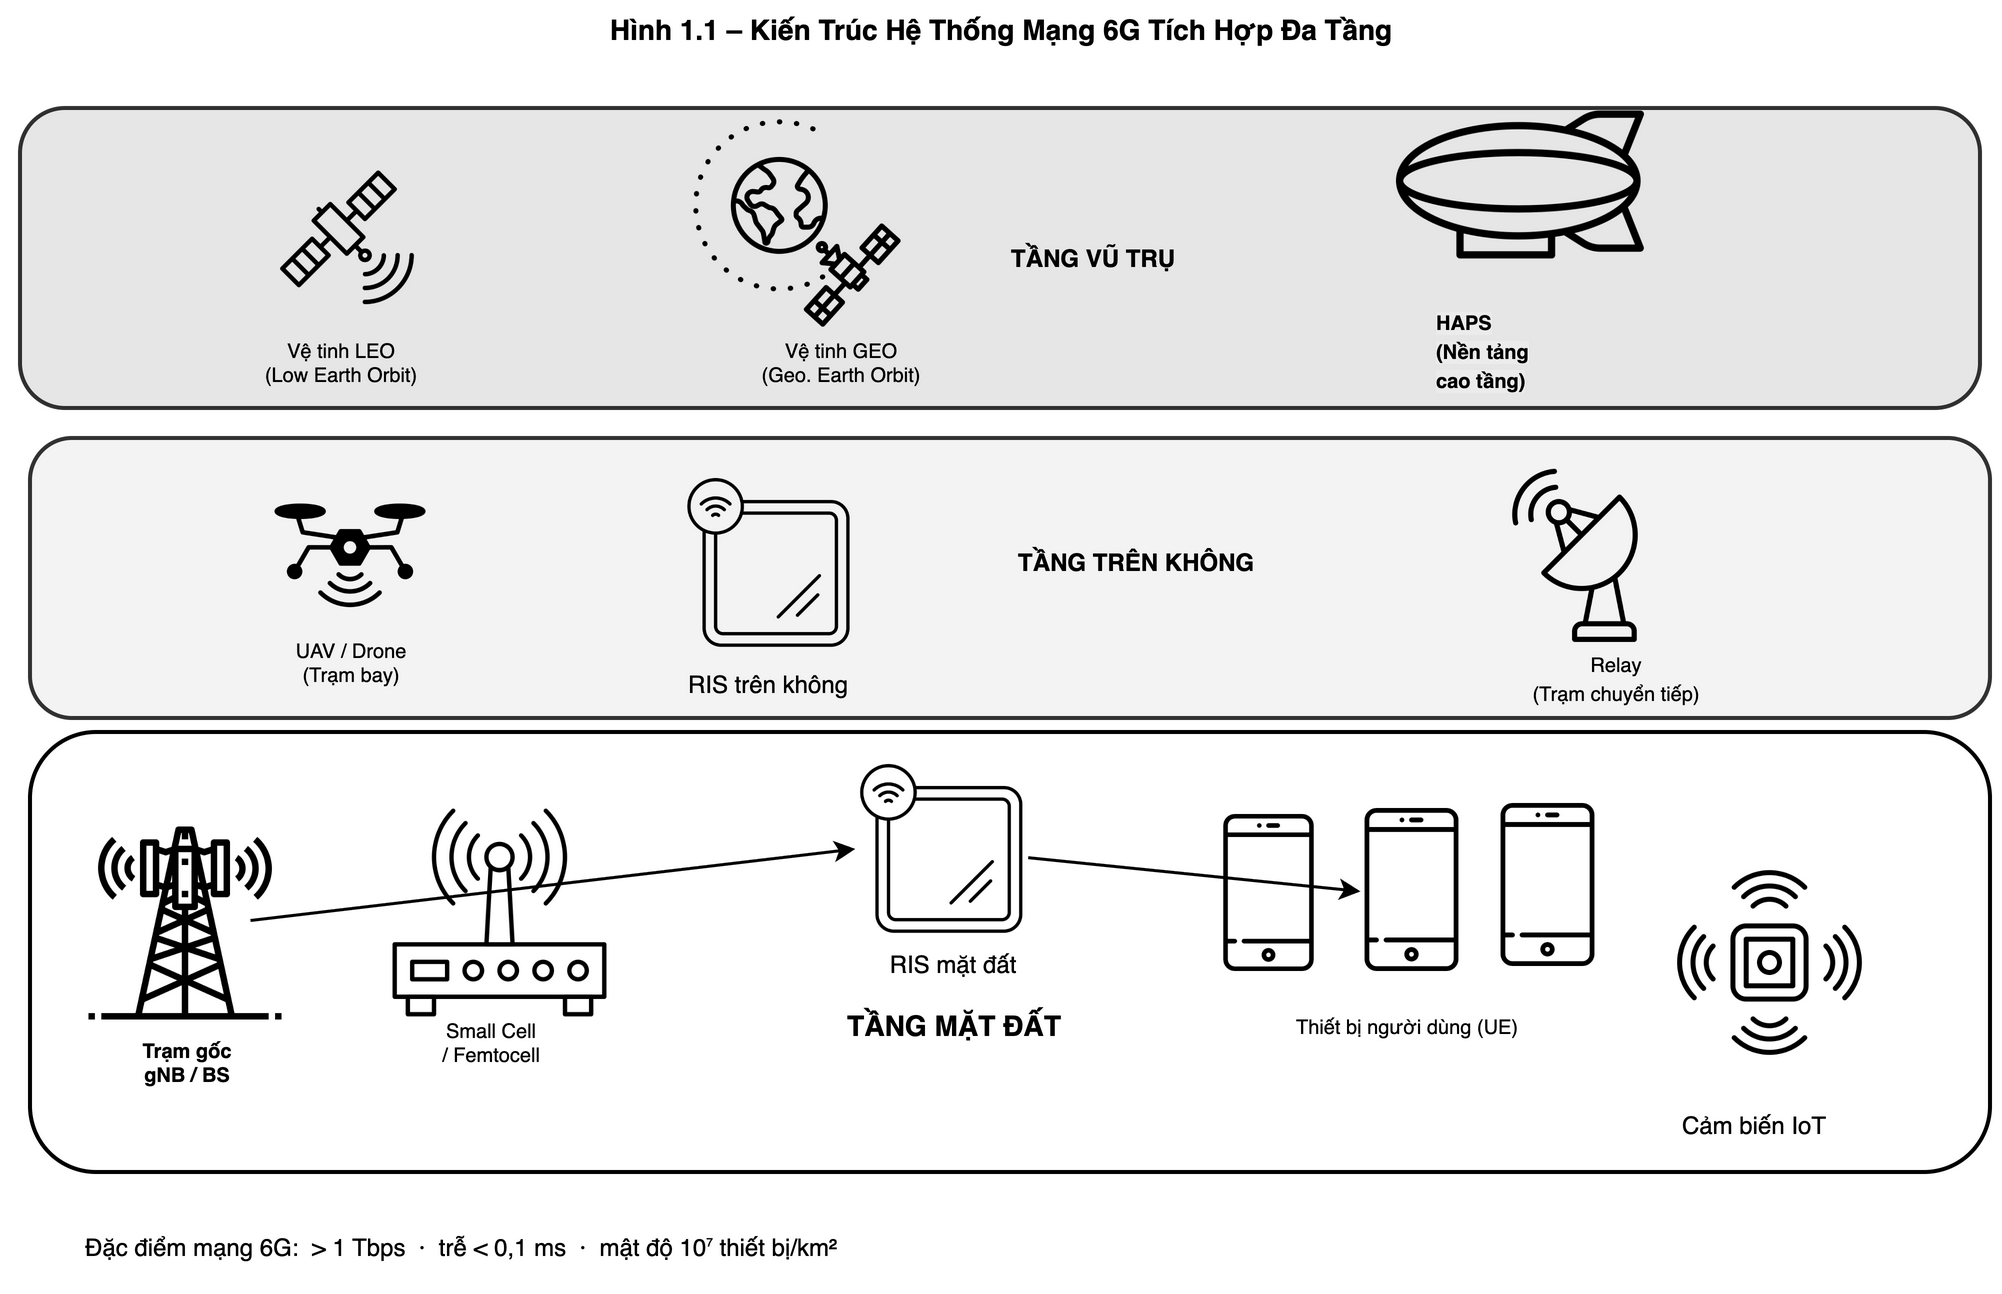
\includegraphics[width=0.92\linewidth]{figures/h1_1_kien_truc_6g.png}
  \caption{Kiến trúc mạng 6G tích hợp đa tầng: vũ trụ, không trung, mặt đất.}
  \label{fig:h1_1}
\end{figure}

So với 5G, các chỉ tiêu của 6G được đặt ra ở mức rất cao
\cite{noor2025aimulti}, \cite{noman2026drl6g}: thông lượng đỉnh trên $1$~Tbps; độ
trễ vô tuyến dưới $100~\mu$s; mật độ kết nối $10^7$ thiết bị/km$^2$; hiệu
quả phổ tăng $10$ lần; hiệu quả năng lượng cải thiện $100$ lần. Để đạt được
các chỉ tiêu này, 6G cần khai thác đồng thời nhiều băng tần (sub-6 GHz,
mmWave, THz), tích hợp trí tuệ nhân tạo ở các tầng vô tuyến và mạng, đồng
thời sử dụng các công nghệ ``điều khiển môi trường truyền sóng''.

\subsection{Thách thức cốt lõi}

Ba thách thức chính cho 6G được nêu trong các báo cáo gần đây
\cite{adams2024rsma}, \cite{priya2024noma}:

\textbf{Khan hiếm phổ tần.} Băng tần dưới 6~GHz đã được khai thác tối đa,
trong khi mmWave và THz tuy có băng thông lớn nhưng chịu suy hao đường
truyền nghiêm trọng và dễ bị che chắn. Cần các kỹ thuật đa truy nhập tiên
tiến vượt qua giới hạn phổ tần.

\textbf{Quản lý nhiễu.} Mật độ kết nối siêu cao ($10^7$ thiết bị/km$^2$)
khiến nhiễu đồng kênh trở thành nút thắt cổ chai. Các kỹ thuật quản lý
nhiễu mềm dẻo (như RSMA) là điều bắt buộc.

\textbf{Hiệu quả năng lượng.} Yêu cầu hiệu quả năng lượng tăng $100$ lần đòi
hỏi các kiến trúc mạng tiêu thụ năng lượng thấp, trong đó RIS thụ động là
một lựa chọn nổi bật \cite{wu2020smart}, \cite{mu2022simultaneously}.

% -----------------------------------------------------------------------------
\section{Kỹ thuật đa truy nhập RSMA}
\label{sec:rsma}

\subsection{Tiến trình phát triển: OMA $\to$ NOMA $\to$ RSMA}

Trong lịch sử các thế hệ vô tuyến, kỹ thuật đa truy nhập đã trải qua nhiều
giai đoạn \cite{mao2022rsma}, \cite{priya2024noma}. Đa truy nhập trực giao
(OMA) như FDMA, TDMA, OFDMA phân bổ tài nguyên (tần số, thời gian, hoặc
sóng mang con) trực giao cho các người dùng. Cách này đảm bảo không có
nhiễu giữa người dùng, nhưng hiệu quả phổ thấp khi số người dùng tăng.
Đa truy nhập không trực giao (NOMA), đặc biệt là NOMA miền công
suất, cho phép nhiều người dùng dùng chung tài nguyên với mức công suất
khác nhau và sử dụng SIC tại phía thu để giải mã liên tiếp. NOMA cải
thiện hiệu quả phổ nhưng nhạy cảm với lỗi pha-đinh, lỗi ước lượng kênh,
và đặc biệt là rất khó tối ưu khi có nhiều người dùng đồng thời cần phục
vụ.

Đa truy nhập theo phân tách tốc độ (RSMA), được Mao và cộng sự
tổng hợp trong \cite{mao2018rsma}, \cite{mao2022rsma}, kết hợp ưu điểm của cả
OMA và NOMA: thông điệp của mỗi người dùng được tách thành phần
chung và phần riêng, truyền chung tài nguyên nhưng với cấu
trúc xử lý hai bậc thay vì xếp tầng tuyến tính như NOMA. Hình \ref{fig:h1_2}
mô tả trực quan sự khác biệt về cách phân bổ tài nguyên giữa OMA, NOMA và
RSMA trong miền tần số/thời gian và công suất. Có thể thấy OMA phân chia
các UE vào các khe tài nguyên trực giao riêng biệt, NOMA chồng các UE
trên cùng tài nguyên với mức công suất khác nhau, còn RSMA bổ sung thêm
một luồng chung được chia sẻ giữa các UE để xử lý nhiễu một cách linh
hoạt hơn.

\begin{figure}[t]
  \centering
  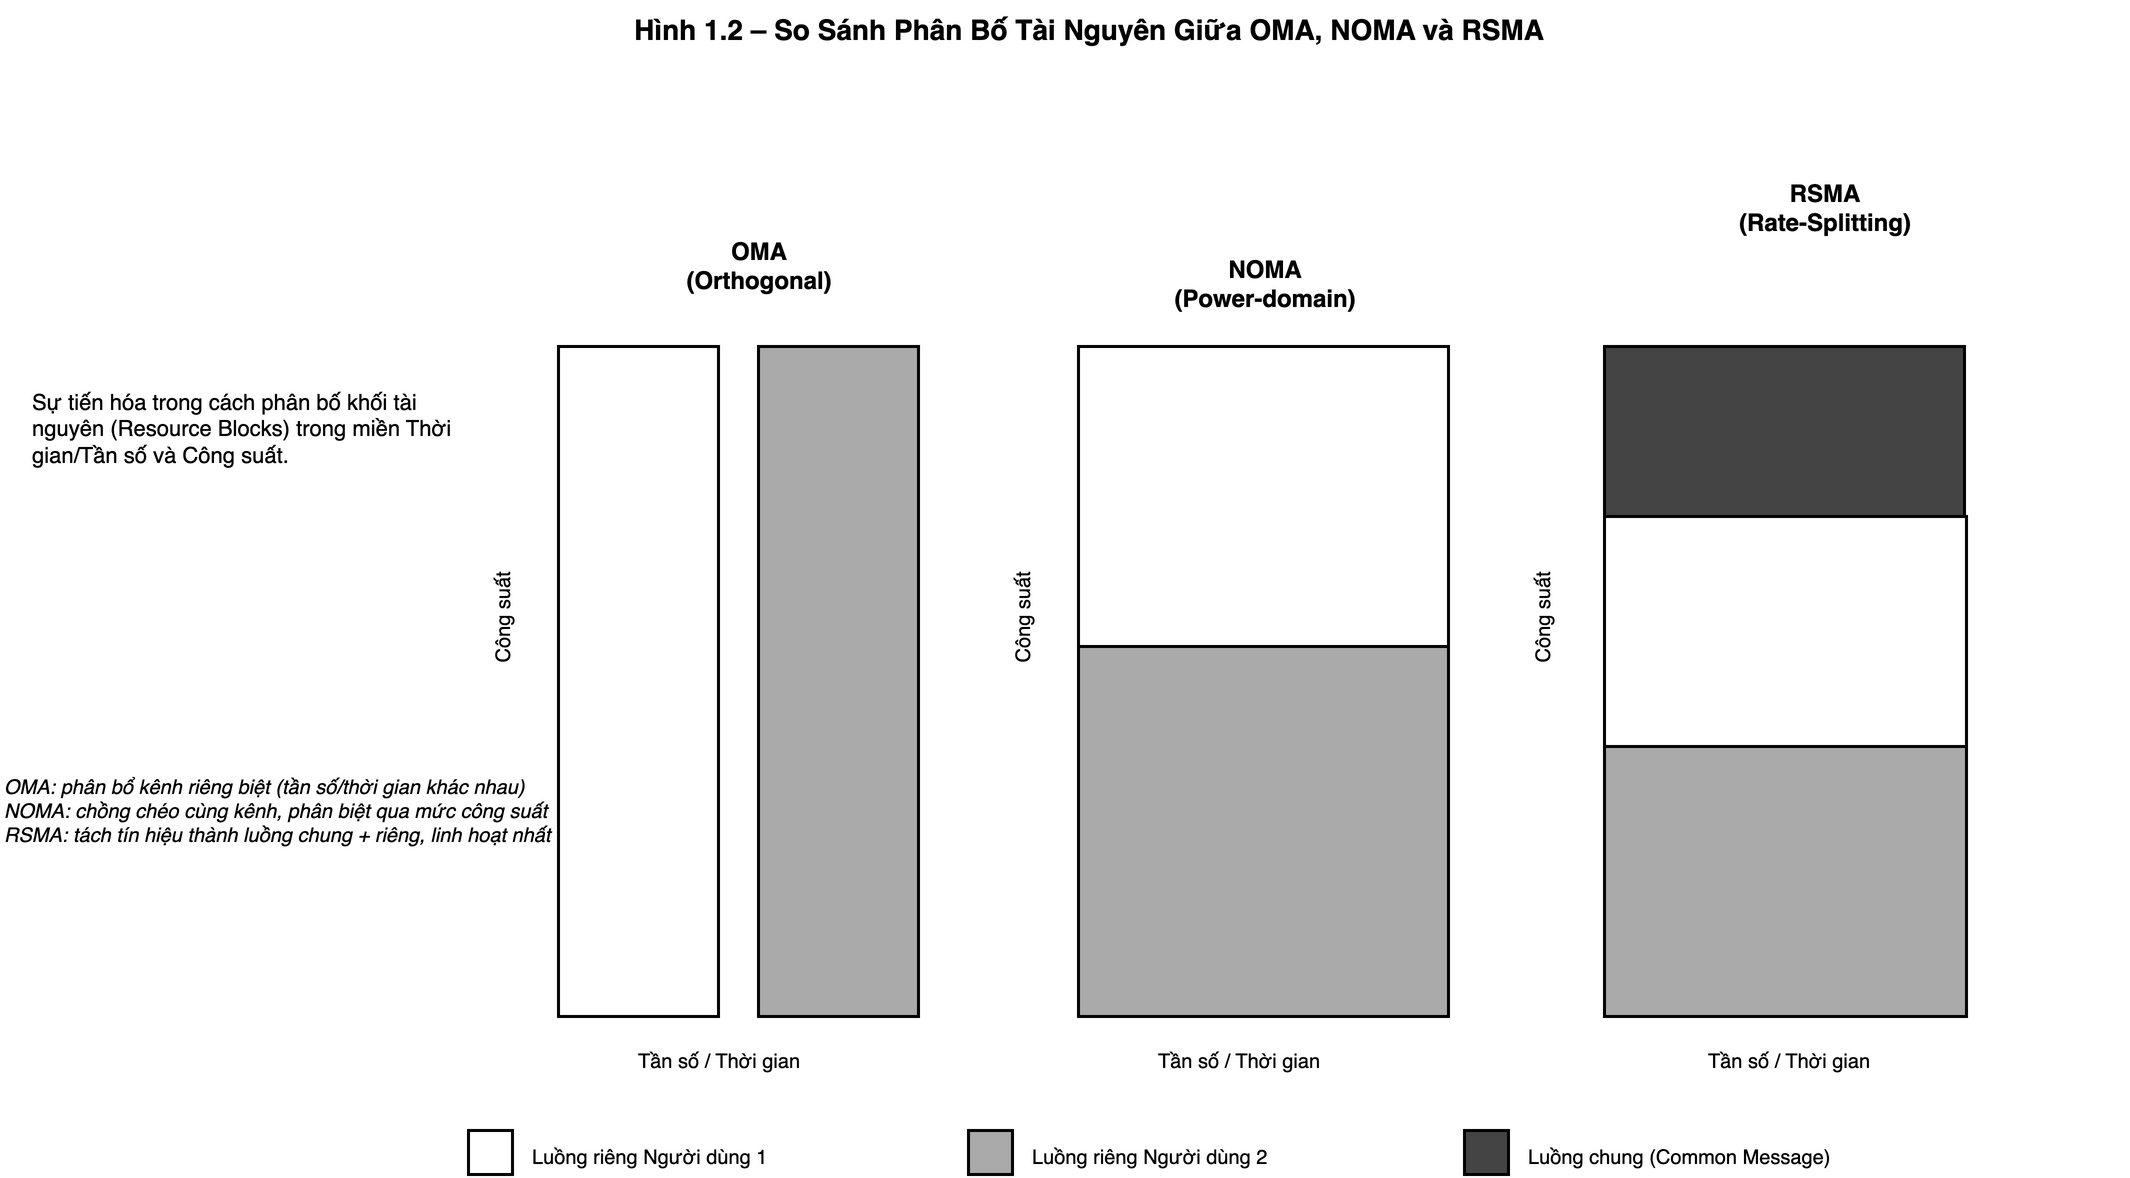
\includegraphics[width=0.95\linewidth]{figures/h1_2_oma_noma_rsma.png}
  \caption{So sánh phân bổ tài nguyên giữa OMA, NOMA và RSMA.}
  \label{fig:h1_2}
\end{figure}

\subsection{Mô hình tín hiệu RSMA lớp đơn}

Xét hệ thống đường xuống một trạm gốc phục vụ $K$ người dùng. Thông điệp
nguyên thủy $W_k$ của người dùng $k$ được tách thành hai phần: phần chung
$W_k^c$ và phần riêng $W_k^p$ \cite{mao2022rsma}, \cite{hua2023learning}. Các
phần chung của tất cả người dùng được kết hợp thành một thông
điệp chung duy nhất $W_c$ rồi mã hóa thành luồng chung $s_c$; các phần
riêng $W_k^p$ được mã hóa độc lập thành các luồng riêng $s_k$. Tín hiệu
phát hợp nhất tại BS có dạng:
\begin{equation}
  x \;=\; \sqrt{P_c}\,s_c \;+\; \sum_{k=1}^{K}\sqrt{P_k}\,s_k,
  \label{eq:rsma_signal}
\end{equation}
trong đó $P_c$ là công suất dành cho luồng chung, $P_k$ là công suất dành
cho luồng riêng của người dùng $k$, với ràng buộc tổng công suất
$P_c + \sum_{k=1}^{K} P_k \le P_{\max}$. Các luồng được chuẩn hóa năng
lượng trung bình đơn vị: $\E\{|s_c|^2\} = \E\{|s_k|^2\} = 1$. Hình
\ref{fig:h1_3} biểu diễn sơ đồ khối xử lý tín hiệu RSMA lớp đơn, gồm bộ
tách thông điệp (Message Splitter), bộ gộp luồng chung (Combiner), bộ mã
hóa và tiền mã hóa (Encoder \& Precoders), khối nhân công suất và bộ
tổng hợp tín hiệu $\Sigma$. Tại phía thu, người dùng giải mã luồng chung
trước, áp dụng khử nhiễu liên tiếp (SIC) và sau đó giải mã luồng riêng
dành riêng cho mình.

\begin{figure}[t]
  \centering
  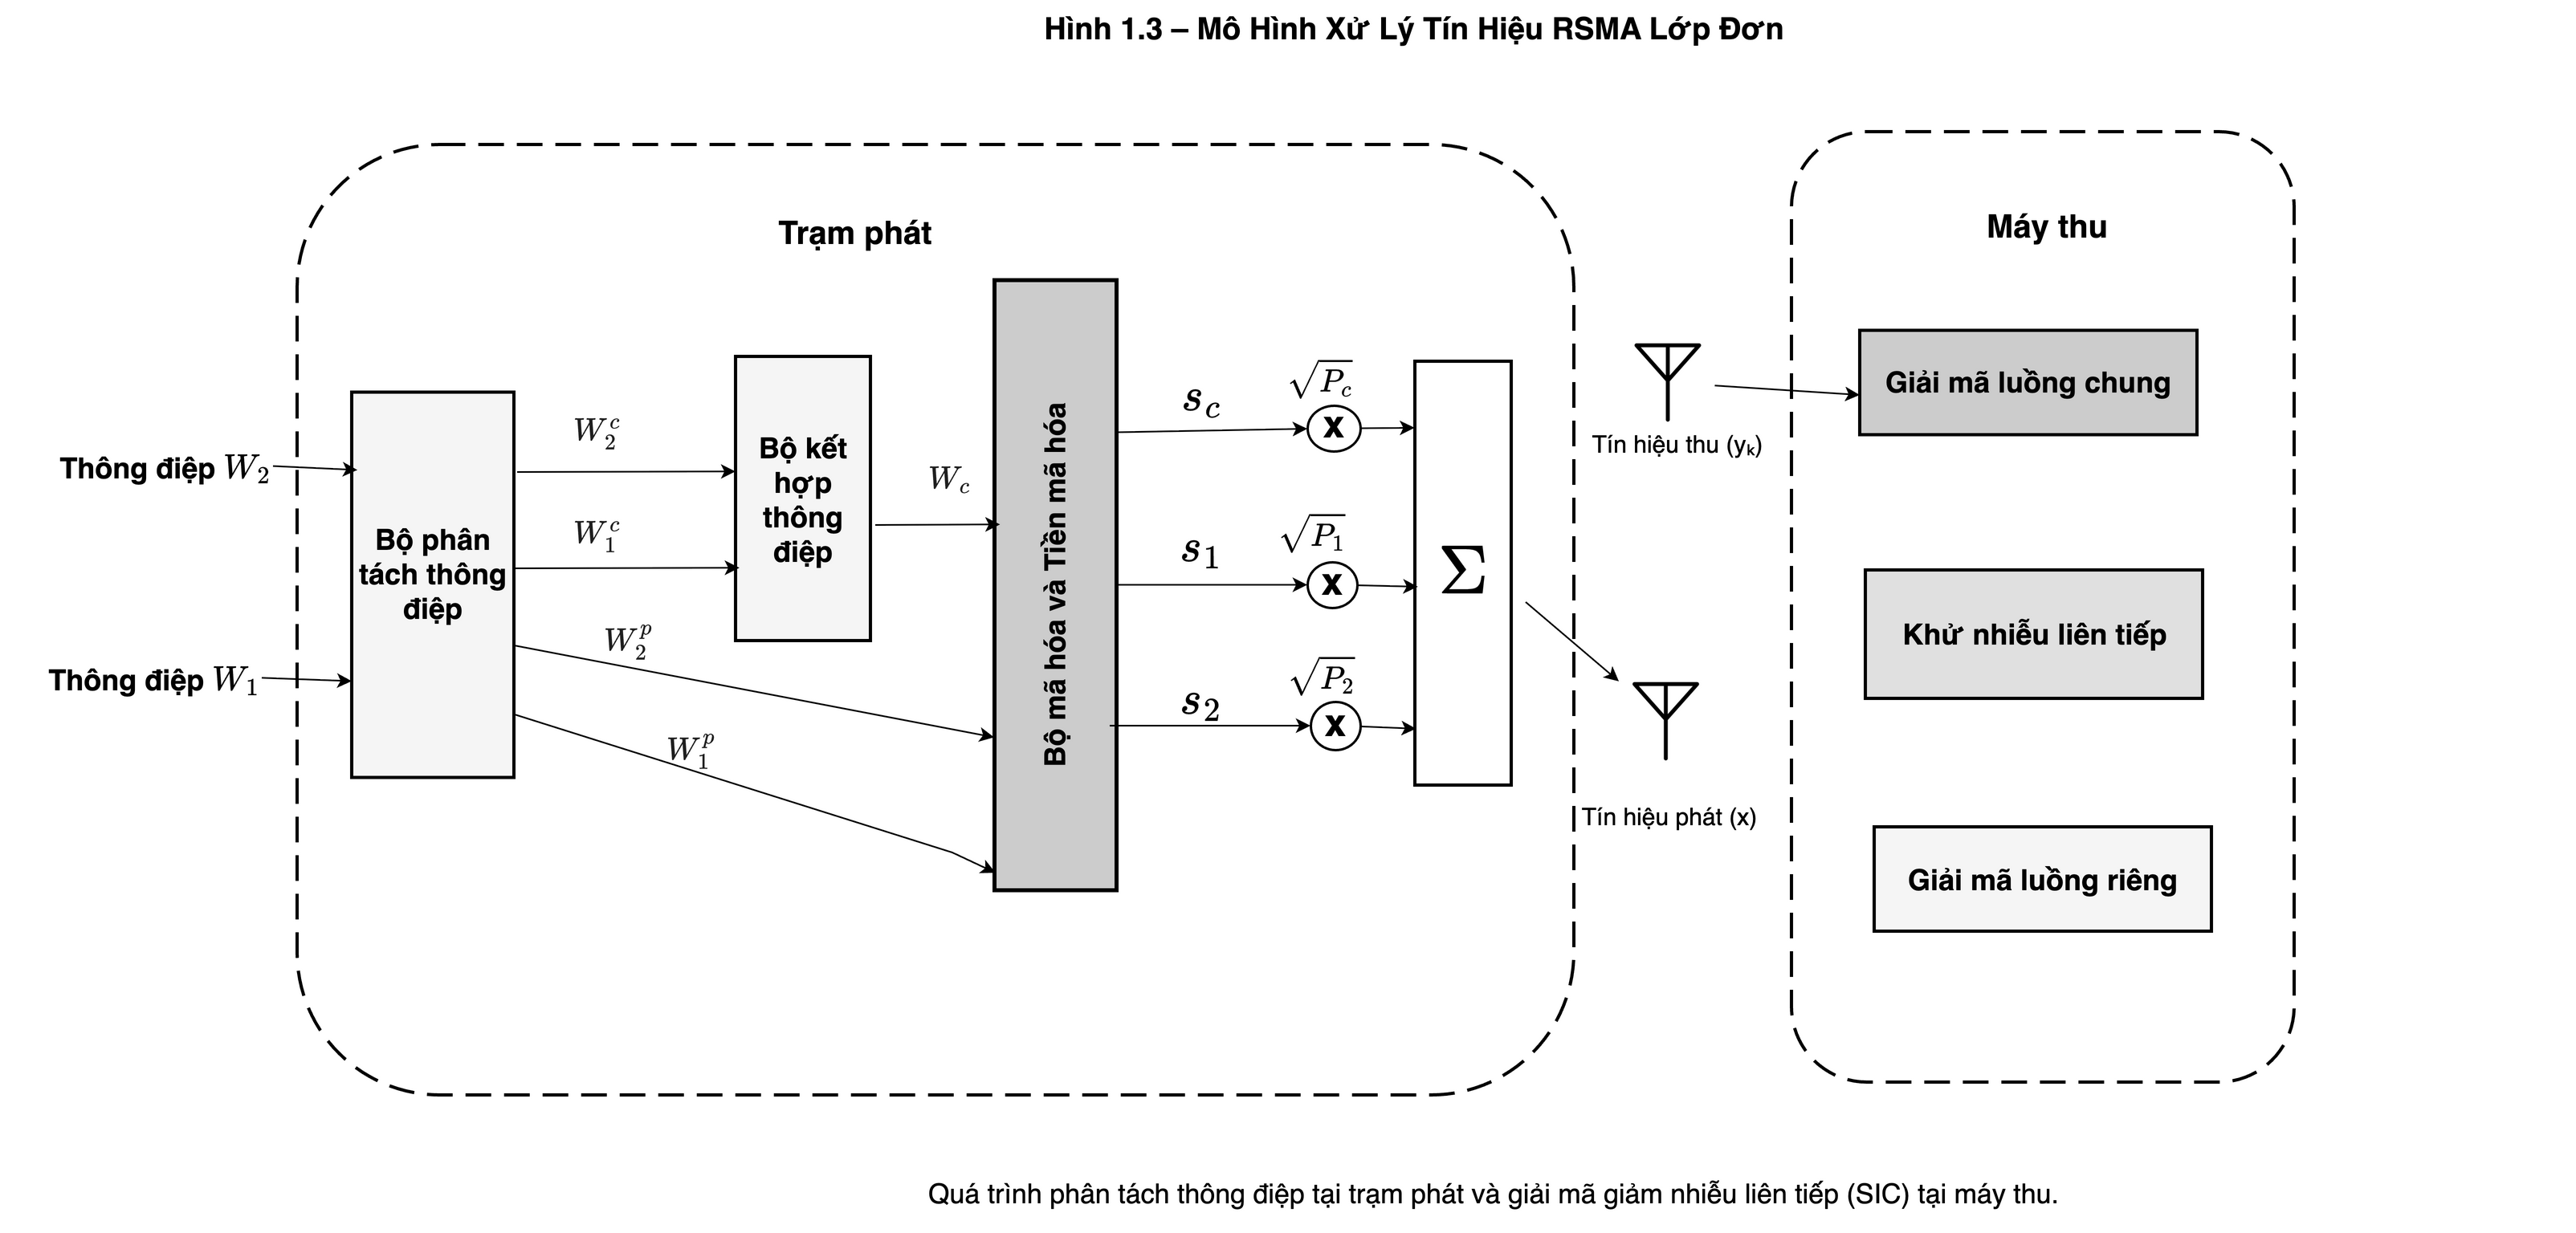
\includegraphics[width=0.95\linewidth]{figures/h1_3_rsma_tin_hieu.png}
  \caption{Sơ đồ khối xử lý tín hiệu RSMA lớp đơn: phía phát (Splitter, Combiner,
  Encoder \& Precoders, $\Sigma$) và phía thu (giải mã luồng chung, SIC, giải mã
  luồng riêng).}
  \label{fig:h1_3}
\end{figure}

Tại phía thu, người dùng $k$ nhận được tín hiệu $y_k$ qua kênh hiệu dụng
$h_{eff,k}$ (sẽ trình bày chi tiết ở chương sau). Quá trình giải mã gồm
hai bước:
\begin{enumerate}[label=(\arabic*),leftmargin=*]
\item Giải mã luồng chung $\hat s_c$, xem các luồng riêng là nhiễu.
\item Áp dụng SIC để trừ ảnh hưởng của $\hat s_c$, sau đó giải mã luồng
riêng $\hat s_k$ dành cho mình, xem các luồng riêng còn lại là nhiễu.
\end{enumerate}

Tốc độ luồng chung của người dùng $k$ là
$R_{c,k} = \log_2(1+\gamma_{c,k})$ với $\gamma_{c,k}$ là SINR luồng chung;
tốc độ luồng riêng là $R_{p,k} = \log_2(1+\gamma_{p,k})$. Vì luồng chung
phải được giải mã thành công bởi mọi người dùng nên tốc độ luồng
chung khả thi bị giới hạn bởi người dùng yếu nhất:
\begin{equation}
  R_c \;=\; \min_{k\in\{1,\ldots,K\}}\, R_{c,k}.
  \label{eq:rc_minmax}
\end{equation}
Tổng tốc độ thu được của người dùng $k$ là
\begin{equation}
  R_k \;=\; c_k\,R_c \;+\; R_{p,k},
  \label{eq:rk}
\end{equation}
trong đó $c_k \in [0,1]$ là tỷ lệ luồng chung phân chia cho người dùng $k$,
thỏa $\sum_{k=1}^K c_k = 1$. Tổng tốc độ toàn hệ thống được định nghĩa là
$R_{\text{sum}} = \sum_{k=1}^{K} R_k$.

\subsection{Ưu điểm RSMA trong quản lý nhiễu}

So với OMA và NOMA, RSMA mang lại ba ưu điểm \cite{mao2022rsma}, \cite{priya2024noma}, \cite{irkicatal2024deep}:

\textbf{(i) Quản lý nhiễu mềm dẻo.} Bằng việc điều chỉnh tỷ lệ tách
$\{c_k\}$ và công suất $\{P_c, P_k\}$, RSMA có thể chuyển trạng thái
giữa hai cực: ``coi nhiễu như tín hiệu mong muốn'' (như SDMA) và ``khử
nhiễu hoàn toàn'' (như NOMA truyền thống). Vì vậy RSMA bao hàm OMA, SDMA
và NOMA như các trường hợp đặc biệt.

\textbf{(ii) Bền vững với lỗi CSI.} RSMA cho phép phía phát đặt một phần
năng lượng vào luồng chung, vốn được giải mã trước khi gặp nhiễu phá
hủy do lỗi CSI, nhờ đó giảm thiểu suy giảm hiệu năng so với NOMA tinh
khiết \cite{wu2024deep}, \cite{cernaloli2023meta}.

\textbf{(iii) Tương thích với SIC một bước.} RSMA chỉ yêu cầu một bước SIC
tại phía thu (giải mã luồng chung trước), đơn giản hơn so với NOMA cần
SIC liên tiếp đối với mỗi cặp người dùng.

% -----------------------------------------------------------------------------
\section{Công nghệ STAR-RIS}
\label{sec:starris}

\subsection{Tổng quan RIS và các giới hạn}

Bề mặt phản xạ thông minh (Reconfigurable Intelligent Surface
RIS) là một mặt phẳng gồm nhiều phần tử thụ động, mỗi phần tử có thể được
điều chỉnh pha (và đôi khi cả biên độ) thông qua các diode PIN hoặc vật
liệu meta. Khi tín hiệu tới mặt phẳng, mỗi phần tử áp dụng một pha dịch
$\phi_n$ trước khi tái phát ra, tạo nên hiệu ứng định dạng tia
``trên không'' mà không cần các bộ khuếch đại RF chủ động
\cite{wu2020smart}. RIS truyền thống chỉ có thể phản xạ tín hiệu, do đó
chỉ phục vụ người dùng nằm trong nửa không gian phía trước RIS
($180^\circ$). Người dùng ở phía sau RIS không nhận được tín hiệu cải
thiện, một hạn chế lớn trong các kịch bản triển khai thực tế.

\subsection{Nguyên lý hoạt động STAR-RIS}

STAR-RIS giải quyết hạn chế trên bằng cách cho phép mỗi phần tử
đồng thời phản xạ một phần năng lượng vào nửa không gian phía
trước (vùng phản xạ R) và truyền qua một phần năng lượng sang nửa không
gian phía sau (vùng truyền qua T), với pha của hai thành phần được điều
chỉnh độc lập \cite{liu2021starris}, \cite{mu2022simultaneously}. Hình
\ref{fig:h1_4} so sánh trực quan vùng phủ của RIS truyền thống với
STAR-RIS, cho thấy STAR-RIS mở rộng vùng phục vụ từ nửa không gian
$180^\circ$ thành toàn không gian $360^\circ$. Điều này đặc biệt có giá
trị trong các kịch bản UE phân bố ở cả hai phía mặt phẳng RIS, như khi
RIS được lắp đặt trên tường tòa nhà hoặc trên thiết bị bay.

\begin{figure}[t]
  \centering
  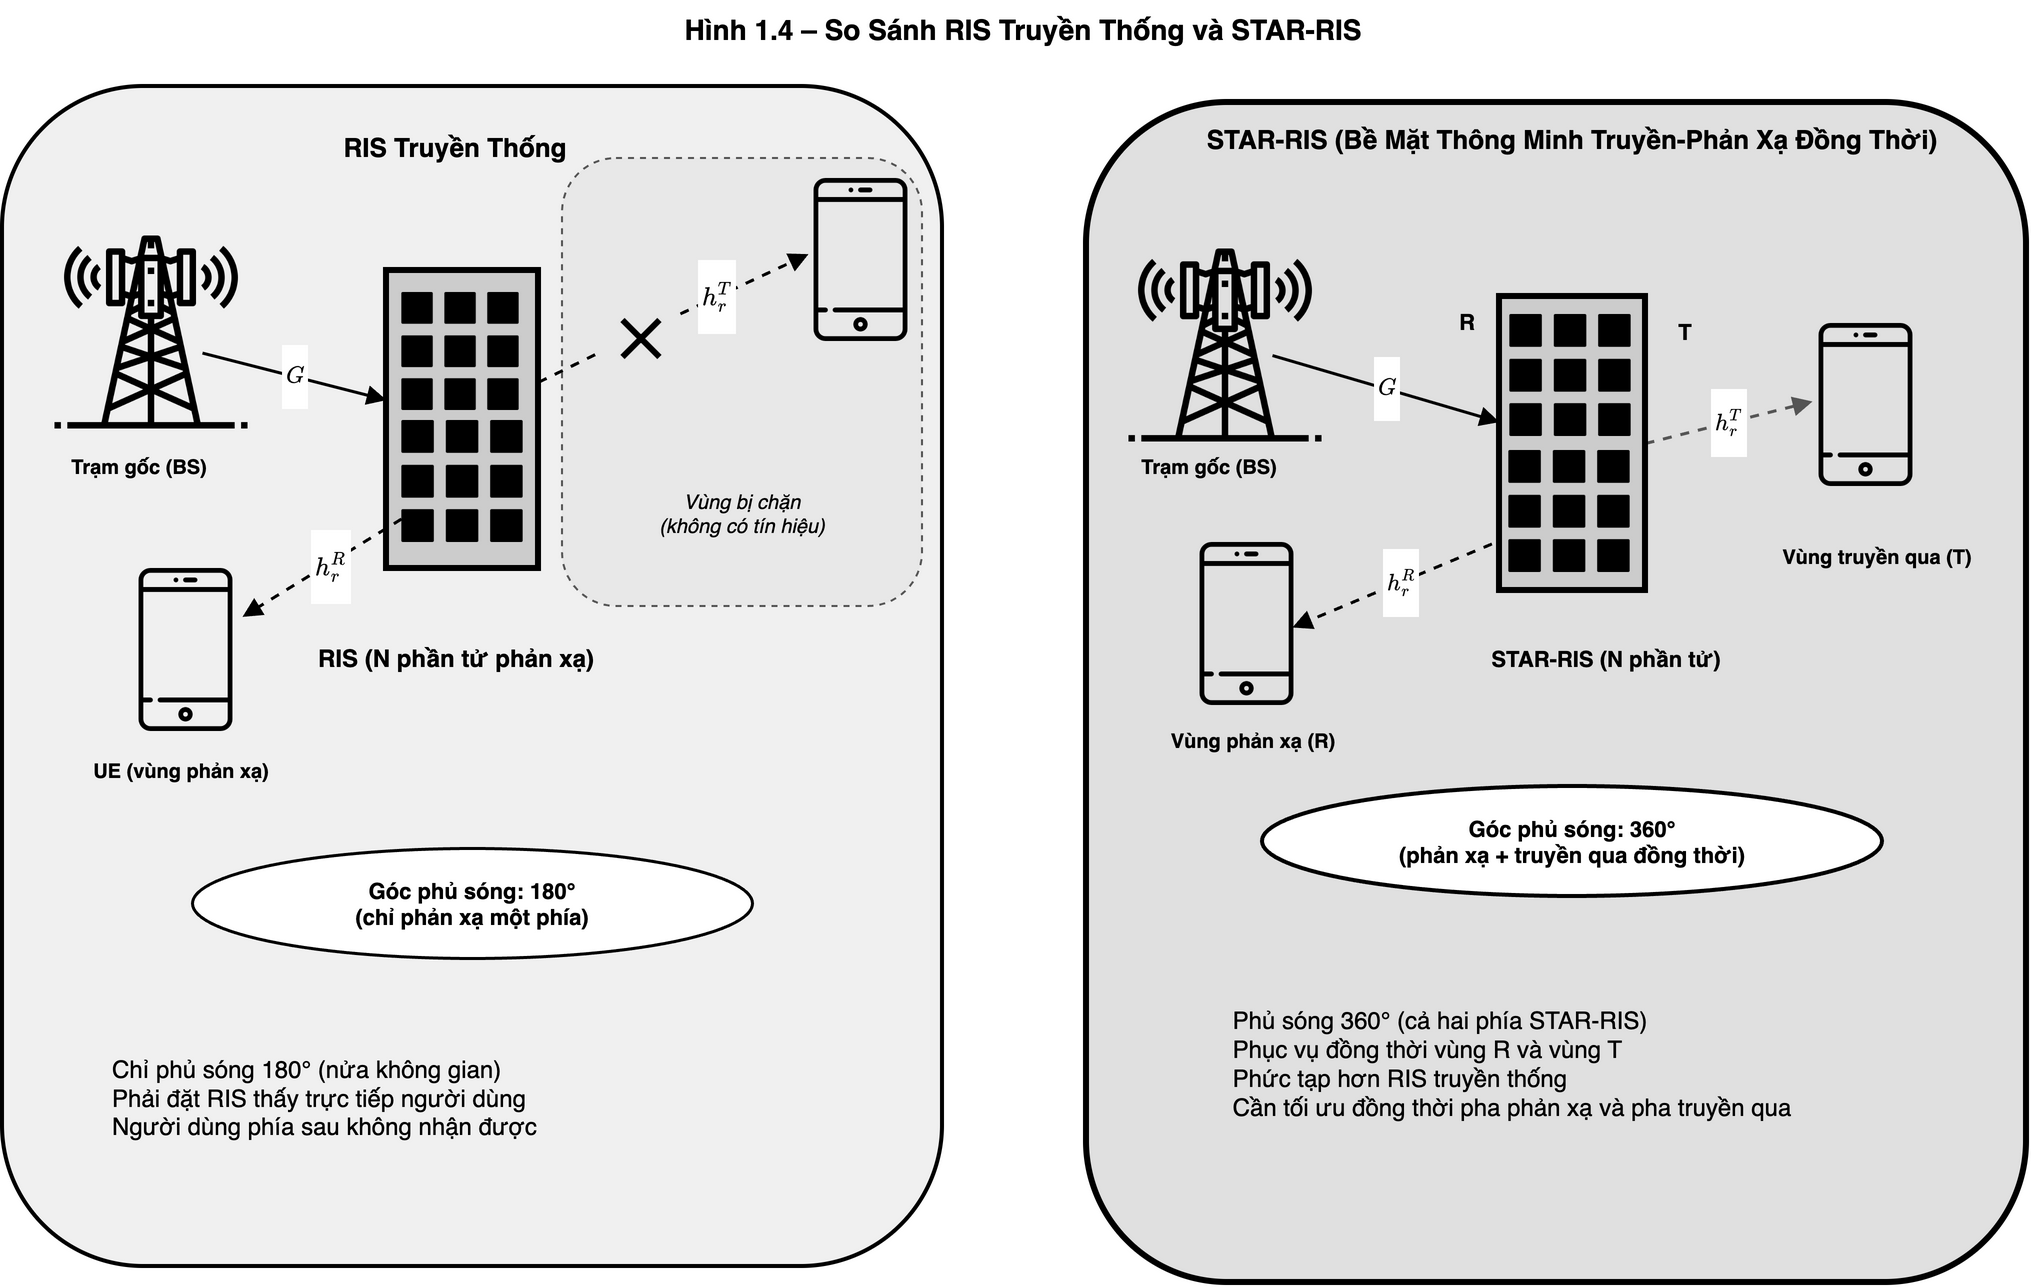
\includegraphics[width=0.92\linewidth]{figures/h1_4_star_ris_vs_ris.png}
  \caption{So sánh vùng phủ sóng: RIS truyền thống ($180^\circ$) và STAR-RIS
  ($360^\circ$). STAR-RIS phục vụ người dùng ở cả hai phía của bề mặt.}
  \label{fig:h1_4}
\end{figure}

Đối với phần tử thứ $n$ của STAR-RIS, hệ số phản xạ và truyền qua được
mô tả bởi các số phức:
\begin{equation}
\Phi_n^R = \sqrt{\beta_n^R}\,e^{j\theta_n^R}, \qquad
\Phi_n^T = \sqrt{\beta_n^T}\,e^{j\theta_n^T},
\label{eq:starris_coef}
\end{equation}
trong đó $\beta_n^R, \beta_n^T \in [0,1]$ là biên độ phản xạ và truyền qua,
$\theta_n^R, \theta_n^T \in [0, 2\pi)$ là pha dịch tương ứng. Bộ điều khiển
STAR-RIS phải điều chỉnh đồng thời $4N$ tham số (hai biên độ và hai pha
cho mỗi phần tử) sao cho cải thiện tổng tốc độ của toàn hệ thống.

\subsection{Ba chế độ vận hành: ES, MS, TS}

STAR-RIS có ba chế độ vận hành cơ bản \cite{mu2022simultaneously}, \cite{liu2021starris}:

\textbf{Chế độ chia sẻ năng lượng (Energy Splitting, ES).} Mỗi phần tử
chia năng lượng tín hiệu tới thành hai phần với tỉ lệ $\beta_n^R$ và
$\beta_n^T$, ràng buộc bởi định luật bảo toàn năng lượng:
\begin{equation}
\beta_n^R + \beta_n^T = 1, \quad \forall n \in \{1,\ldots,N\}.
\label{eq:es_constraint}
\end{equation}
ES là chế độ tổng quát nhất, cho phép STAR-RIS phục vụ đồng thời cả hai
vùng. Đây cũng là chế độ được sử dụng trong Luận văn.

\textbf{Chế độ chuyển đổi chế độ (Mode Switching, MS).} Mỗi phần tử
hoạt động ở một trong hai trạng thái nhị phân: phản xạ thuần
($\beta_n^R = 1, \beta_n^T = 0$) hoặc truyền qua thuần. Mặc dù đơn giản
về phần cứng nhưng MS không khai thác hết khả năng của STAR-RIS.

\textbf{Chế độ chuyển đổi thời gian (Time Switching, TS).} Bề mặt
chuyển toàn bộ phần tử giữa phản xạ và truyền qua theo các khe thời gian,
phù hợp khi yêu cầu phục vụ hai vùng không cần đồng thời.

\subsection{Ứng dụng STAR-RIS trong mạng 6G}

Trong những năm gần đây, STAR-RIS đã được ứng dụng vào nhiều kịch bản 6G:
truyền thông an toàn \cite{kamal2024optimizing}, \cite{zhang2024starrismatrans}, \cite{yang2024covertambc}, truyền thông UAV \cite{singh2024robust}, \cite{perdana2024adaptive}, \cite{huang2024starrisuav}, \cite{nguyen2025star}, truyền thông tích hợp cảm biến
(ISAC) \cite{jin2024arisrsma}, \cite{to2024fairness}, \cite{adams2024rsma},
URLLC \cite{soleymani2024starris}, SWIPT \cite{amiri2024meta}, và nhiều
ứng dụng khác. Trong số đó, kết hợp STAR-RIS với RSMA đã được chứng minh
là tăng hiệu năng đáng kể cho mạng đường xuống \cite{soleymani2024starris}, \cite{gomes2024performance}, \cite{ibrahim2025cognitive}.

% -----------------------------------------------------------------------------
\section{Phân bổ tài nguyên: phương pháp truyền thống và động lực chuyển sang DRL}
\label{sec:resource_allocation}

\subsection{Các phương pháp tối ưu cổ điển}

Bài toán phân bổ tài nguyên cho mạng RIS-RSMA thường có dạng tối ưu phi
lồi nhiều biến (công suất, pha RIS, hệ số tách luồng). Một số phương pháp
cổ điển được sử dụng \cite{mao2022rsma}, \cite{gomes2024performance}:

\begin{itemize}[leftmargin=*]
\item \textbf{Hạ dần khối tọa độ (BCD):} chia tập biến thành các khối, tối
ưu xen kẽ từng khối khi cố định các khối khác. Hội tụ về điểm dừng cục bộ.
\item \textbf{Nới lỏng nửa xác định (SDR):} chuyển biến pha thành ma trận
hạng một, nới lỏng ràng buộc hạng để bài toán trở nên lồi, sau đó dùng
phép phân rã ngẫu nhiên để truy xuất nghiệm xấp xỉ.
\item \textbf{Lập trình lồi xen kẽ (Alternating Convex Optimization, ACO):}
xen kẽ giải nhiều bài toán con lồi nhỏ.
\end{itemize}

\subsection{Hạn chế của phương pháp truyền thống và động lực DRL}

Các phương pháp trên có chung những hạn chế khi áp dụng vào kịch bản
thực tế \cite{noman2026drl6g}, \cite{hieu2021optimal}, \cite{irkicatal2024deep}:

\textbf{Chi phí tính toán cao.} Mỗi vòng lặp BCD/SDR yêu cầu giải nhiều
bài toán lồi phụ trợ, không khả thi cho cập nhật theo thời gian thực khi
kênh truyền biến thiên ở thang ms.

\textbf{Phụ thuộc vào mô hình kênh tường minh.} Khi mô hình kênh sai
lệch (do hardware impairment, lượng tử hóa pha RIS, lỗi ước lượng kênh),
nghiệm tối ưu hóa truyền thống có thể trở nên rất kém.

\textbf{Khó mở rộng quy mô.} Khi $N$ và $K$ tăng (chẳng hạn $N=256$ phần
tử RIS), độ phức tạp tăng phi tuyến mạnh.

Học tăng cường sâu (DRL) khắc phục các hạn chế trên bằng cách học
chính sách phân bổ tài nguyên từ tương tác với môi trường mô phỏng
\cite{sutton2018reinforcement}, \cite{mnih2015human}, \cite{lillicrap2016continuous}.
Sau khi huấn luyện, suy luận chỉ là một lần chạy tiến của mạng nơ-ron với
độ phức tạp $O(1)$ theo kích thước hệ thống đã cố định trước. DRL cũng
học được đặc trưng quan trọng từ dữ liệu thay vì dựa hoàn toàn vào mô
hình giải tích, do đó bền vững hơn trước nhiễu mô hình
\cite{diamanti2023energy}, \cite{faramarzi2024meta}.

% -----------------------------------------------------------------------------
\section{Học tăng cường sâu (DRL)}
\label{sec:drl}

\subsection{Khung tổng quát của học tăng cường}

Học tăng cường được mô hình hóa dưới dạng quá trình ra quyết định Markov
(MDP), được mô tả bởi bộ năm
$\mathcal{M} = (\mathcal{S}, \mathcal{A}, \mathcal{P}, \mathcal{R}, \gamma)$,
trong đó $\mathcal{S}$ là không gian trạng thái, $\mathcal{A}$ là không
gian hành động, $\mathcal{P}(s_{t+1} | s_t, a_t)$ là hàm chuyển trạng
thái, $\mathcal{R}(s_t, a_t)$ là hàm phần thưởng và $\gamma \in [0,1)$ là
hệ số chiết khấu \cite{sutton2018reinforcement}. Tại mỗi bước thời gian
$t$, tác tử quan sát trạng thái $s_t$, chọn hành động $a_t$ theo chính
sách $\pi(a_t | s_t)$, nhận phần thưởng $r_t$ và chuyển sang trạng thái
mới $s_{t+1}$. Mục tiêu của tác tử là tối đa hóa tổng phần thưởng tích lũy
kỳ vọng:
\begin{equation}
  J(\pi) \;=\; \E_\pi\!\left[\sum_{t=0}^{\infty} \gamma^t r_t\right].
  \label{eq:rl_objective}
\end{equation}
Hình \ref{fig:h1_5} minh họa vòng lặp tương tác giữa tác tử và môi trường
theo khung tổng quát của RL. Mũi tên đi ra từ tác tử biểu diễn hành động
$a_t$ được áp dụng vào môi trường, trong khi mũi tên phản hồi từ môi
trường về tác tử mang theo trạng thái mới $s_{t+1}$ và phần thưởng tức
thời $r_{t+1}$.

\begin{figure}[t]
  \centering
  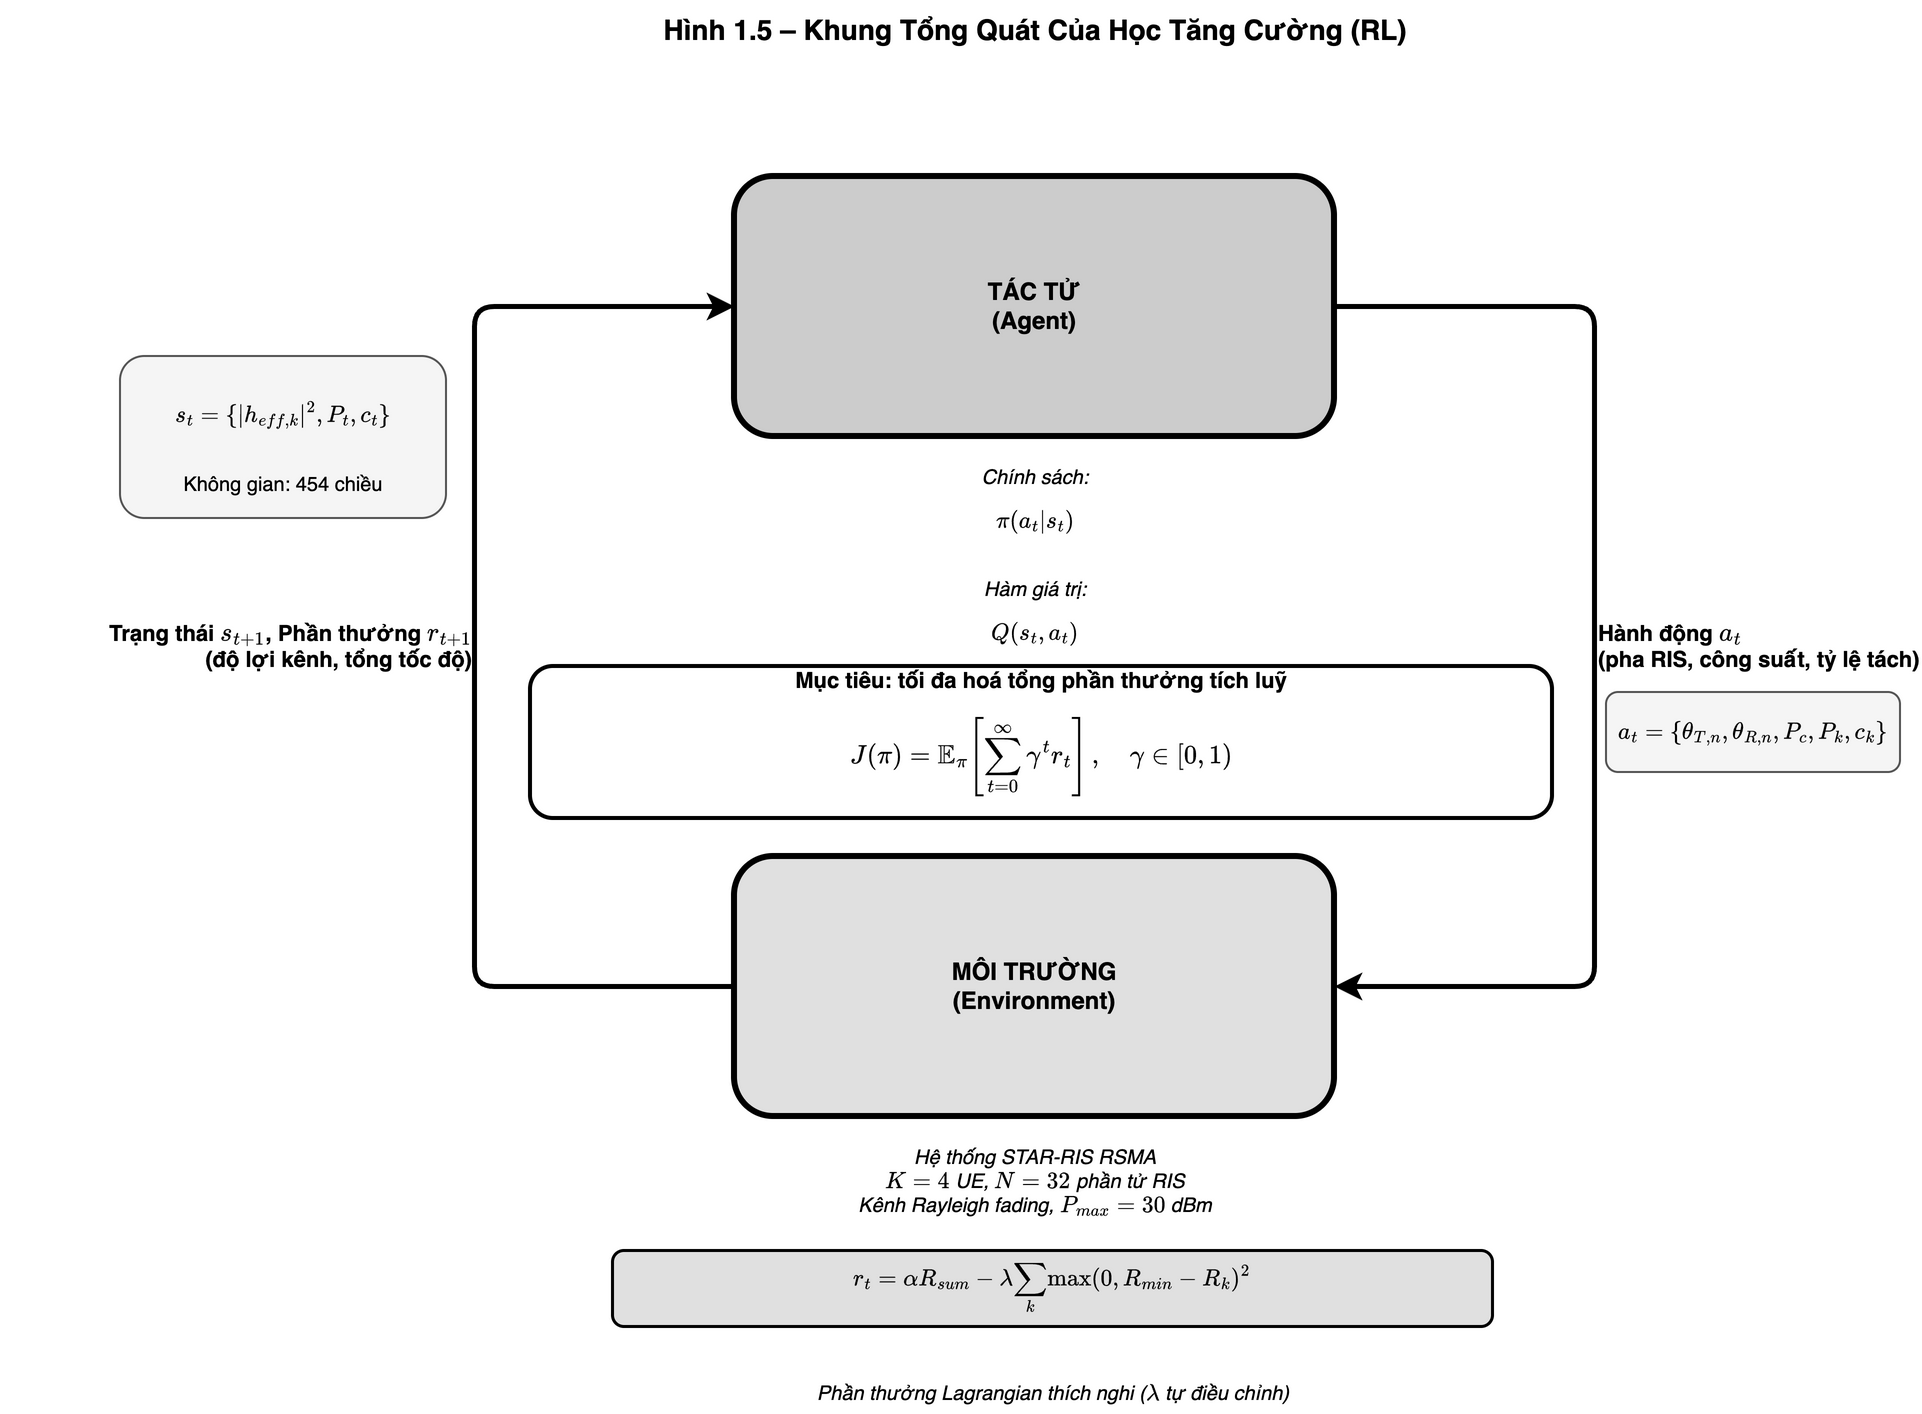
\includegraphics[width=0.78\linewidth]{figures/h1_5_vong_lap_rl.png}
  \caption{Vòng lặp tương tác trong học tăng cường: tác tử quan sát trạng thái,
  chọn hành động, môi trường phản hồi trạng thái mới và phần thưởng.}
  \label{fig:h1_5}
\end{figure}

\subsection{Từ Q-learning đến DQN}

Một trong những thuật toán RL kinh điển nhất là Q-learning, ước lượng
hàm giá trị hành động $Q(s,a)$, là kỳ vọng tổng phần thưởng tích lũy
khi bắt đầu từ trạng thái $s$ và chọn hành động $a$, thông qua phương
trình Bellman:
\begin{equation}
\begin{aligned}
  Q(s,a) \;\leftarrow\;& Q(s,a) \\
  & + \alpha\,\big[\,r + \gamma \max_{a'} Q(s',a') - Q(s,a)\,\big].
\end{aligned}
\end{equation}
Khi không gian trạng thái lớn, Q-learning bảng không khả thi. Mnih và cộng
sự \cite{mnih2015human} đề xuất Deep Q-Network (DQN) sử dụng mạng nơ-ron
sâu để xấp xỉ $Q(s,a)$, mở ra kỷ nguyên DRL. DQN giải quyết được nhiều
bài toán game Atari với mức độ ngang ngửa con người. Tuy nhiên, DQN chỉ
phù hợp với không gian hành động rời rạc.

\subsection{Phương pháp Actor-Critic và DDPG}

Đối với không gian hành động liên tục (như công suất phát, pha RIS),
phương pháp Actor-Critic là lựa chọn tự nhiên. Trong Actor-Critic, có hai
mạng nơ-ron riêng biệt: Actor $\mu_\theta(s)$ học chính sách trực
tiếp, còn Critic $Q_\phi(s,a)$ học hàm giá trị để dẫn dắt huấn
luyện Actor.

Deep Deterministic Policy Gradient (DDPG) \cite{lillicrap2016continuous}
là phiên bản off-policy của Actor-Critic dành cho hành động liên tục, kết
hợp ý tưởng của DQN (replay buffer + target network) với chính sách tất
định. DDPG được cập nhật như sau:
\begin{align}
  \mathcal{L}_{\text{critic}}(\phi) &= \E\big[(Q_\phi(s,a) - y)^2\big],
  \quad y = r + \gamma\,Q_{\phi'}(s', \mu_{\theta'}(s')), \\
  \nabla_\theta J &= \E\big[\nabla_a Q_\phi(s,a)|_{a=\mu_\theta(s)}\,
  \nabla_\theta \mu_\theta(s)\big].
\end{align}
Cập nhật mềm cho mạng mục tiêu:
$\theta' \leftarrow \tau\theta + (1-\tau)\theta'$ với $\tau \ll 1$.

Cải tiến của DDPG bao gồm Twin Delayed DDPG (TD3)
\cite{fujimoto2018addressing} với hai Critic và trì hoãn cập nhật Actor để
giảm sai số overestimation, và Proximal Policy Optimisation (PPO)
\cite{schulman2017proximal} với cập nhật on-policy bị giới hạn để tăng
tính ổn định.

% -----------------------------------------------------------------------------
\section{Thuật toán MADDPG}
\label{sec:maddpg}

\subsection{Bài toán RL đa tác tử}

Khi hệ thống cần được điều khiển bởi nhiều tác tử (ví dụ: BS, STAR-RIS-R,
STAR-RIS-T), bài toán trở thành RL đa tác tử (MARL). Khi áp dụng DDPG
trực tiếp cho từng tác tử (decentralized DDPG), môi trường nhìn từ một
tác tử trở nên không ổn định (non-stationary) vì các tác tử khác
cũng đang thay đổi chính sách. Điều này phá vỡ giả định Markov cố định
và dẫn đến hội tụ kém \cite{lowe2017multi}, \cite{dange2026collaborative}.

\subsection{Cơ chế CTDE trong MADDPG}

Multi-Agent DDPG (MADDPG) đề xuất bởi Lowe và cộng sự
\cite{lowe2017multi} giải quyết vấn đề không ổn định bằng cơ chế
Centralised Training, Decentralised Execution (CTDE):

\textbf{Giai đoạn huấn luyện tập trung.} Mỗi tác tử $i$ có một
Actor $\mu_i$ chỉ thấy quan sát cục bộ $o_i$, nhưng có một
Critic $Q_i$ tập trung thấy toàn bộ quan sát
$\mathbf{o} = (o_1, \ldots, o_N)$ và toàn bộ hành động
$\mathbf{a} = (a_1, \ldots, a_N)$. Vì Critic biết hành động của tất cả
tác tử, môi trường nhìn từ Critic luôn ổn định.

\textbf{Giai đoạn thực thi phân tán.} Sau khi huấn luyện xong, Critic
được bỏ đi; mỗi Actor chỉ cần quan sát cục bộ $o_i$ để sinh ra hành
động $a_i$, không cần thông tin toàn cục. Điều này giúp MADDPG có thể
triển khai trong các kịch bản phân tán thực tế nơi mỗi tác tử chỉ có
quyền truy cập vào thông tin cục bộ. Hình \ref{fig:h1_6} minh họa rõ
hai giai đoạn của cơ chế CTDE, trong đó vùng huấn luyện và vùng thực
thi được tách biệt rõ ràng.

\begin{figure}[t]
  \centering
  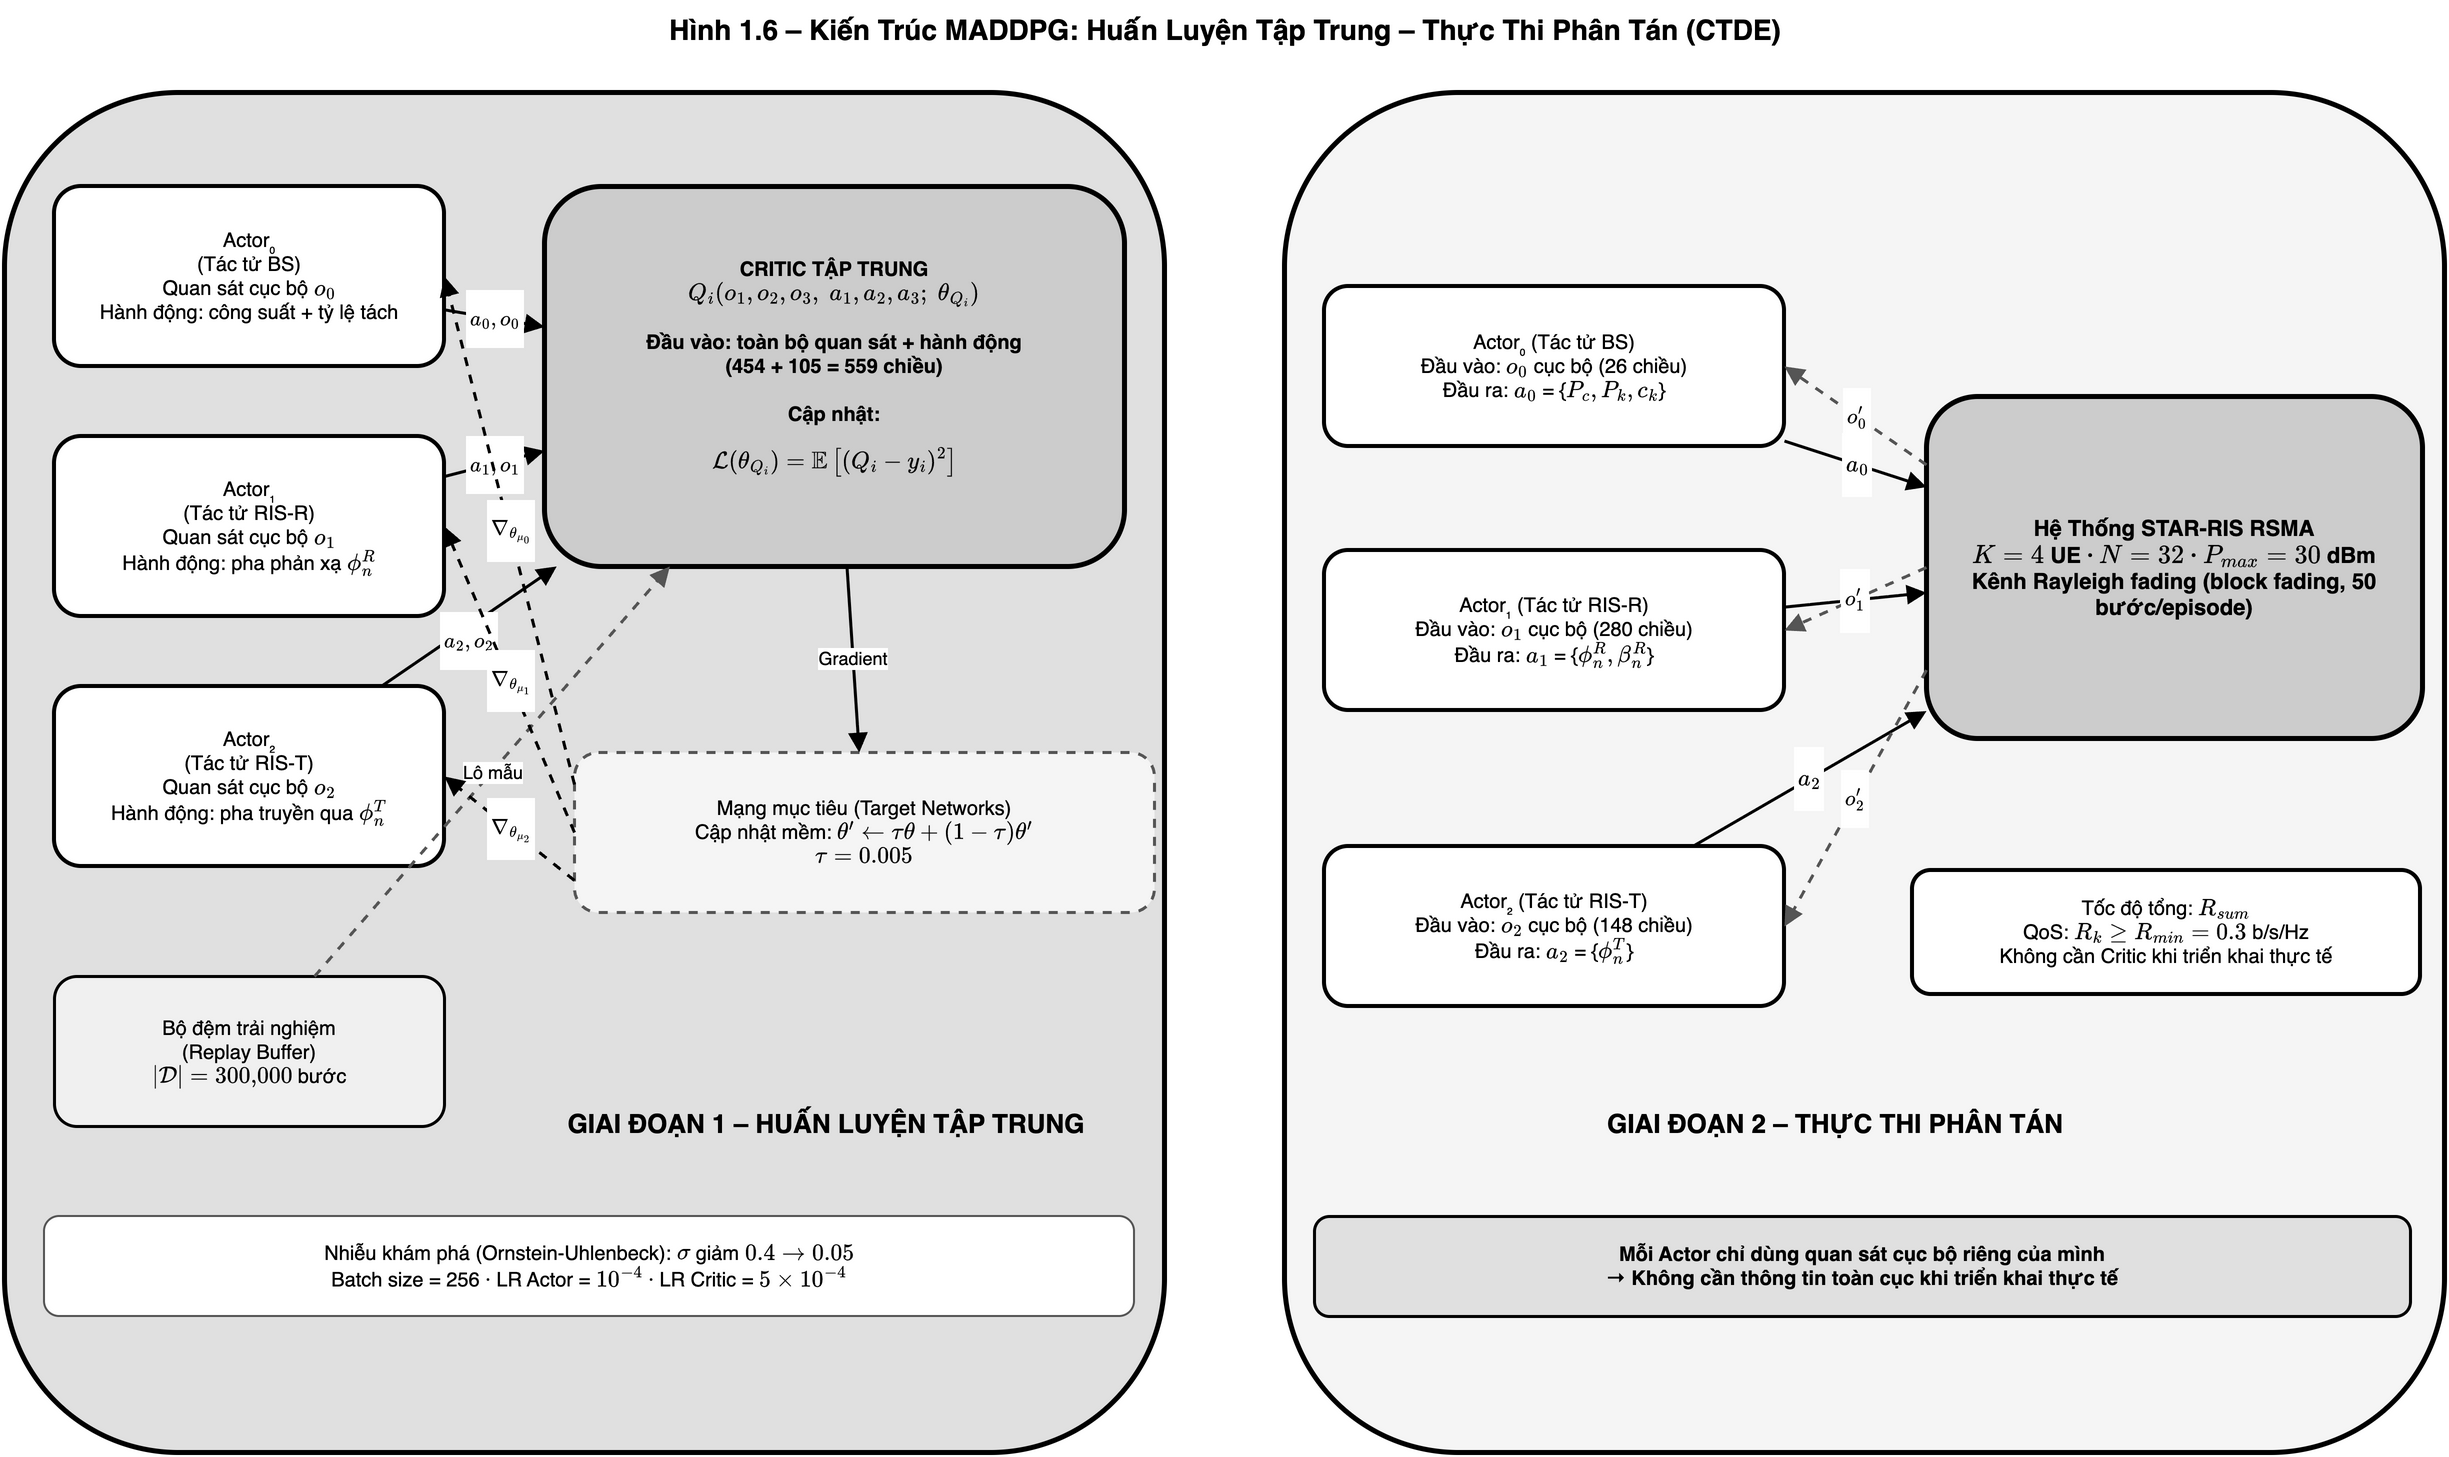
\includegraphics[width=0.95\linewidth]{figures/h1_6_maddpg_ctde.png}
  \caption{Kiến trúc MADDPG với cơ chế CTDE: giai đoạn huấn luyện tập trung
  sử dụng Critic toàn cục, giai đoạn thực thi phân tán chỉ dùng các Actor
  với quan sát cục bộ.}
  \label{fig:h1_6}
\end{figure}

\subsection{So sánh MADDPG với các thuật toán DRL khác}

Bảng \ref{tab:so_sanh_drl} tóm lược ưu nhược điểm của MADDPG so với các
thuật toán DRL phổ biến trong các ứng dụng phân bổ tài nguyên không dây.
Việc so sánh tập trung vào bốn tiêu chí: số lượng tác tử hỗ trợ, ưu điểm
chính, hạn chế chính, và khả năng áp dụng cho không gian hành động liên
tục.

\begin{table}[t]
\centering
\caption{So sánh MADDPG với các thuật toán DRL khác trong phân bổ tài nguyên.}
\label{tab:so_sanh_drl}
\begin{tabular}{p{2.5cm} p{2cm} p{4cm} p{4.5cm}}
\toprule
\textbf{Thuật toán} & \textbf{Số tác tử} & \textbf{Ưu điểm} & \textbf{Hạn chế} \\
\midrule
DQN \cite{mnih2015human}     & 1 & Đơn giản, hội tụ tốt cho hành động rời rạc & Không hỗ trợ hành động liên tục \\
DDPG \cite{lillicrap2016continuous} & 1 & Hành động liên tục, off-policy & Không ổn định khi nhiều tác tử \\
TD3 \cite{fujimoto2018addressing}   & 1 & Khắc phục overestimation của DDPG & Vẫn là đơn tác tử \\
PPO \cite{schulman2017proximal}     & 1 & Cập nhật ổn định, dễ điều chỉnh & On-policy nên kém hiệu quả mẫu \\
\textbf{MADDPG} \cite{lowe2017multi} & $\geq 2$ & CTDE, ổn định trong môi trường đa tác tử & Critic tập trung tăng theo số tác tử \\
\bottomrule
\end{tabular}
\end{table}

MADDPG đã được ứng dụng thành công cho nhiều bài toán không dây gần
đây: phân bổ tài nguyên trong RIS-NOMA \cite{mirza2024multi},
SWIPT-STAR-RIS \cite{dange2026collaborative}, và là cơ sở để Luận
văn này phát triển khuôn khổ phân bổ tài nguyên trong STAR-RIS-RSMA.

% -----------------------------------------------------------------------------
\section{Khoảng trống nghiên cứu và động lực}
\label{sec:research_gap}

Phần này tổng hợp các hạn chế của ba hướng tiếp cận hiện hành đối với
bài toán phân bổ tài nguyên trong mạng STAR-RIS RSMA, từ đó xác định
khoảng trống nghiên cứu (research gap) mà Luận văn hướng tới.

\subsection{Hạn chế của RSMA độc lập}

RSMA độc lập, nghĩa là RSMA không kết hợp với RIS, đã được chứng minh
là vượt trội OMA và NOMA về quản lý nhiễu trong cấu hình MISO/MIMO
\cite{mao2018rsma}, \cite{mao2022rsma}. Tuy nhiên, khi UE nằm trong vùng
NLoS hoặc bị chướng ngại vật che chắn, kênh hiệu dụng suy giảm nghiêm
trọng (xấp xỉ $-25$ dB trong các đánh giá điển hình), khiến luồng chung
$R_c = \min_k R_{c,k}$ bị giới hạn bởi người dùng yếu nhất. Nói cách
khác, RSMA độc lập không cải thiện được điều kiện truyền sóng vật lý
mà chỉ cải thiện việc xử lý nhiễu, do đó hiệu năng vẫn bị giới hạn bởi
kênh truyền cơ sở.

\subsection{Hạn chế của tối ưu STAR-RIS truyền thống}

Các phương pháp tối ưu cổ điển cho STAR-RIS như tối ưu xen kẽ
(Alternating Optimization, AO), hạ dần khối tọa độ (Block Coordinate
Descent, BCD) và nới lỏng nửa xác định (Semidefinite Relaxation, SDR)
yêu cầu giải nhiều bài toán lồi phụ trợ trong mỗi vòng lặp
\cite{wu2020smart}, \cite{soleymani2024starris}. Với $N$ phần tử
STAR-RIS, mỗi vòng SDR có độ phức tạp $\mathcal{O}(N^6)$ hoặc cao hơn,
trong khi BCD đặc trưng cần $50$--$100$ vòng lặp để hội tụ. Tổng chi
phí tính toán này không phù hợp với yêu cầu thời gian thực của 6G, nơi
khoảng coherence kênh chỉ kéo dài cỡ vài mili-giây. Hơn nữa, các phương
pháp này yêu cầu hiểu biết tường minh về mô hình kênh và thường phải
được thiết kế lại khi cấu hình hệ thống thay đổi.

\subsection{Hạn chế của DRL đơn tác tử}

DRL đơn tác tử (như DDPG, TD3, PPO) áp dụng cho bài toán P0 đặt toàn
bộ không gian hành động vào một mạng Actor duy nhất. Với $N=32$ và
$K=4$, không gian hành động hợp nhất có $105$ chiều, bao gồm các đại
lượng có ý nghĩa vật lý hoàn toàn khác nhau: công suất phát $\{P_c,
P_k\}$, tỷ lệ phân chia $\{c_k\}$, pha và biên độ STAR-RIS $\{\theta_n^X,
\beta_n^R\}$. Tác tử đơn không khai thác được cấu trúc phân rã tự nhiên
của bài toán, dẫn đến không gian khám phá lớn và độ phức tạp huấn luyện
cao. Kết quả thực nghiệm trong Chương \ref{ch:chuong4} (Bảng
\ref{tab:algorithm_comparison}) sẽ định lượng hệ quả này: DDPG đơn tác
tử chỉ đạt sum-rate $1{,}98$ b/s/Hz so với $3{,}41$ b/s/Hz của khuôn
khổ đa tác tử đề xuất; hơn nữa, thí nghiệm quét theo $N$ cho thấy
khoảng cách giữa tác tử đơn tốt nhất (TD3) và khuôn khổ đa tác tử
tăng dần theo kích thước không gian hành động, đạt $+0{,}83$ b/s/Hz
tại $N=96$.

\subsection{Khoảng trống nghiên cứu xác định}

Tổng hợp ba hạn chế trên, một khoảng trống nghiên cứu rõ rệt được nhận
diện: \emph{thiếu một khuôn khổ tối ưu chung cho mạng STAR-RIS RSMA
đồng thời đáp ứng bốn đặc tính (i) tối ưu tài nguyên đa miền (công suất,
pha, biên độ, tỷ lệ tách), (ii) xử lý ràng buộc QoS từng người dùng qua
một surrogate ràng buộc mềm với cập nhật đối ngẫu, (iii)
tính khả thi thời gian thực, và (iv) suy luận thời gian thực điều kiện
theo CSI tức thời (real-time CSI-conditioned inference) trong mô hình
kênh động Gauss--Markov.} Luận văn này lấp đầy khoảng trống đó bằng cách
đề xuất khuôn khổ MADDPG-CTDE ba tác tử chuyên dụng. Việc lựa chọn
MADDPG được biện minh từ ba góc độ: cơ chế CTDE giải quyết tính không
ổn định của môi trường đa tác tử thường gặp khi áp dụng DDPG độc lập
cho mỗi tác tử \cite{lowe2017multi}; phân rã ba tác tử khớp tự nhiên
với cấu trúc bài toán (BS điều khiển công suất, RIS-R điều khiển pha
phản xạ, RIS-T điều khiển pha truyền qua); không gian hành động được
ghép cặp (coupled) cũng được phản ánh đúng qua phần thưởng chia sẻ
trong khung cooperative MARL.

% -----------------------------------------------------------------------------
\section{So sánh với các công trình liên quan}
\label{sec:related_work}

Bảng \ref{tab:related_work} so sánh Luận văn này với các công trình
gần đây trên bảy phương diện chủ yếu. Mỗi cột tương ứng với một đặc
tính kỹ thuật quan trọng, từ đó cho phép định vị rõ ràng đóng góp của
Luận văn so với văn liệu hiện tại.

\begin{table}[t]
\centering
\small
\caption{So sánh Luận văn này với các công trình liên quan.}
\label{tab:related_work}
\setlength{\tabcolsep}{4pt}
\begin{tabular}{lccccccc}
\toprule
\textbf{Công trình} & \textbf{STAR-RIS} & \textbf{RSMA} & \textbf{DRL} & \textbf{Đa tác tử} & \textbf{QoS} & \textbf{Mốc AO} & \textbf{CSI-cond.} \\
                    &                   &                &              & \textbf{(MARL)}     &              &              & \textbf{infer.}  \\
\midrule
\cite{mao2022rsma}        & --- & $\checkmark$ & ---           & ---           & ---           & ---           & ---           \\
\cite{liu2021starris}     & $\checkmark$ & --- & ---           & ---           & ---           & ---           & ---           \\
\cite{hieu2021optimal}    & --- & $\checkmark$ & $\checkmark$ & ---           & ---           & ---           & $\checkmark$ \\
\cite{hua2023learning}    & --- & $\checkmark$ & $\checkmark$ & ---           & ---           & ---           & $\checkmark$ \\
\cite{wu2024deep}         & --- & $\checkmark$ & $\checkmark$ & ---           & ---           & ---           & $\checkmark$ \\
\cite{soleymani2024starris}& $\checkmark$ & $\checkmark$ & --- & ---  & ---           & $\checkmark$ & ---           \\
\cite{gomes2024performance}& $\checkmark$ & $\checkmark$ & --- & ---  & ---           & ---           & ---           \\
\cite{amiri2024meta}      & $\checkmark$ & $\checkmark$ & $\checkmark$ & ---           & ---           & ---           & $\checkmark$ \\
\cite{bao2025heuristic}   & $\checkmark$ & $\checkmark$ & $\checkmark$ & ---           & ---           & ---           & $\checkmark$ \\
\cite{diamanti2023energy} & --- & $\checkmark$ & $\checkmark$ & ---           & $\checkmark$ & ---           & $\checkmark$ \\
\cite{huang2024starrisuav}& $\checkmark$ & --- & $\checkmark$ & ---           & ---           & ---           & $\checkmark$ \\
\cite{dange2026collaborative}& $\checkmark$ & --- & $\checkmark$ & $\checkmark$ & ---           & ---           & $\checkmark$ \\
\cite{faramarzi2024meta}  & $\checkmark$ & $\checkmark$ & $\checkmark$ & ---           & ---           & ---           & $\checkmark$ \\
\midrule
\textbf{Luận văn này}     & $\checkmark$ & $\checkmark$ & $\checkmark$ & $\checkmark$ & $\checkmark$ & $\checkmark$ & $\checkmark$ \\
\bottomrule
\end{tabular}

\vspace{0.2em}
{\footnotesize Ghi chú: $\checkmark$ chỉ ra phương diện được xử lý trong công trình. Cột ``Mốc AO'' biểu thị có sử dụng phương pháp tối ưu xen kẽ (AO/BCD) làm mốc so sánh (không phải cận trên). Cột ``CSI-cond. infer.'' biểu thị khả năng suy luận thời gian thực điều kiện theo CSI tức thời tại thời gian chạy.\par}
\hfill {\footnotesize\itshape Nguồn: Tác giả tổng hợp (2026)}
\end{table}


Quan sát Bảng \ref{tab:related_work} cho thấy phần lớn các công trình
hiện hành chỉ xử lý hai hoặc ba trong bảy phương diện. Các công trình
RSMA cổ điển \cite{mao2022rsma} không xét RIS, trong khi các công trình
RIS-RSMA dùng phương pháp tối ưu cổ điển \cite{soleymani2024starris},
\cite{gomes2024performance} phải giải lại bài toán tối ưu lặp cho từng
thể hiện kênh nên khó đáp ứng thời gian thực. Các
công trình DRL cho RSMA \cite{hieu2021optimal}, \cite{hua2023learning},
\cite{wu2024deep} thường chỉ dùng đơn tác tử và không xét STAR-RIS.
Các công trình STAR-RIS với DRL \cite{huang2024starrisuav},
\cite{dange2026collaborative} chưa kết hợp với RSMA. Đặc biệt, ràng
buộc QoS từng UE và việc dùng một heuristic tối ưu xen kẽ (AO-Grid)
làm mốc so sánh cổ điển là hai đặc tính ít được khảo sát đồng thời
trong các nghiên cứu STAR-RIS RSMA. Luận văn này định vị mình là công
trình kết hợp cả bảy phương diện trong một khuôn khổ thống nhất, đặc
biệt với cơ chế phần thưởng Lagrangian surrogate có các hệ số phạt
$\lambda_k$ per-user cập nhật bằng projected dual gradient.

% -----------------------------------------------------------------------------
\section*{Kết luận chương}
\addcontentsline{toc}{section}{Kết luận chương}

Chương 1 đã cung cấp nền tảng lý thuyết tổng quan cho Luận văn, bao gồm:
yêu cầu khắt khe của 6G; nguyên lý hoạt động của RSMA với mô hình tín hiệu
phân tách thành luồng chung và luồng riêng, sử dụng SIC tại phía thu;
kiến trúc STAR-RIS với ba chế độ vận hành (tập trung vào ES); khuôn khổ
DRL và đặc biệt là thuật toán MADDPG với cơ chế CTDE. Các nội dung này là
cơ sở để Chương 2 xây dựng mô hình hệ thống và phát biểu bài toán tối ưu
P0, đồng thời là tiền đề cho Chương 3 thiết kế khuôn khổ MADDPG đề xuất.


% Chương 2
% =============================================================================
%  CHƯƠNG 2 – MÔ HÌNH HỆ THỐNG VÀ BÀI TOÁN TỐI ƯU
% =============================================================================
\chapter{MÔ HÌNH HỆ THỐNG VÀ BÀI TOÁN TỐI ƯU}
\label{ch:chuong2}

Chương này trình bày chi tiết mô hình hệ thống STAR-RIS hỗ trợ RSMA được
xem xét trong Luận văn, các giả thiết cơ bản, mô hình kênh truyền, mô
hình tín hiệu, tính toán SINR và tốc độ, phát biểu bài toán tối ưu (P0)
và cuối cùng là ánh xạ bài toán P0 sang quá trình ra quyết định Markov
(MDP) để áp dụng MADDPG ở Chương 3.

% -----------------------------------------------------------------------------
\section{Cấu hình hệ thống}
\label{sec:cau_hinh}

\subsection{Mô hình hệ thống và các giả thiết}

Hệ thống được xét bao gồm: một trạm gốc (BS) với $M=1$ anten (cấu hình
SISO), một STAR-RIS với $N=32$ phần tử thụ động hoạt động ở chế độ chia
sẻ năng lượng (ES), và $K=4$ thiết bị người dùng (UE) được phân thành hai
nhóm: $K_R=3$ người dùng trong vùng phản xạ R và $K_T=1$ người dùng
trong vùng truyền qua T \cite{liu2021starris}, \cite{mu2022simultaneously}, \cite{soleymani2024starris}. Hình \ref{fig:h2_1} minh họa cấu hình hệ thống, trong đó BS đặt cố định một phía của STAR-RIS, các UE phân bố ở cả hai vùng R và T. Người dùng vùng T chịu suy hao chướng ngại $-25$ dB trên đường truyền trực tiếp, mô phỏng kịch bản NLoS điển hình nơi STAR-RIS thực sự cần thiết để cung cấp kết nối tin cậy.

\begin{figure}[t]
  \centering
  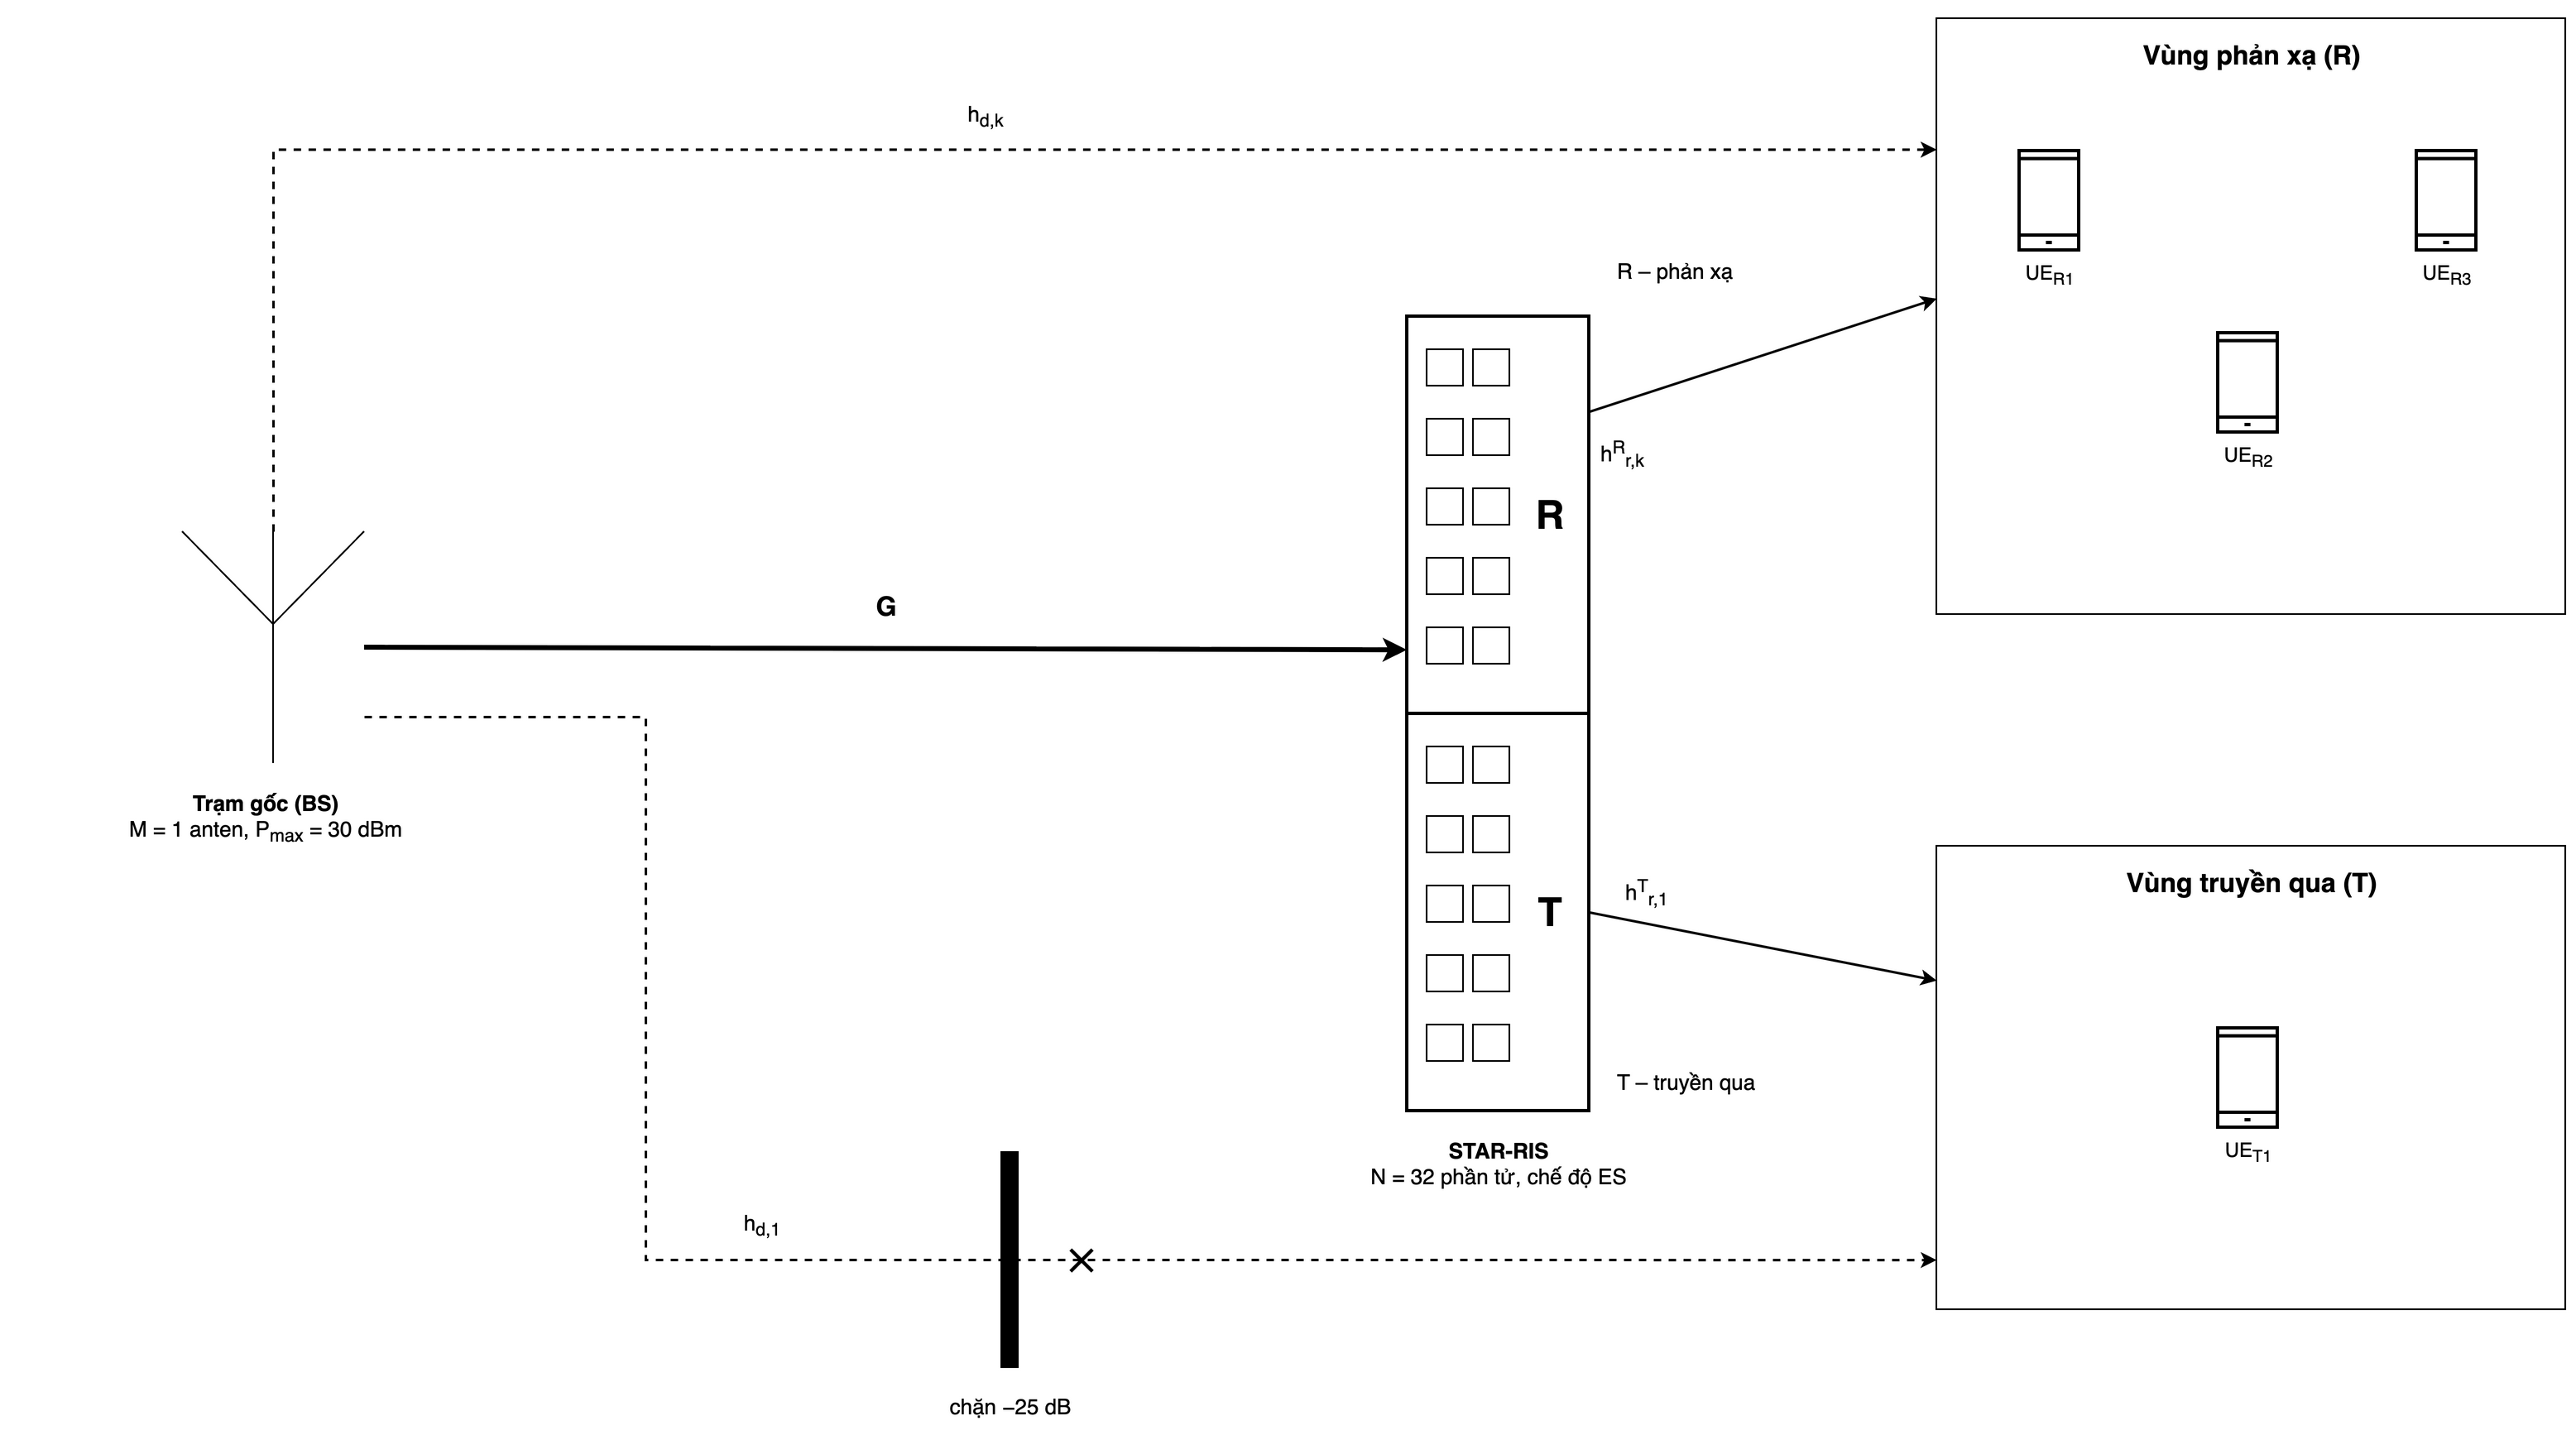
\includegraphics[width=0.96\linewidth]{figures/h2_1_cau_hinh_he_thong.png}
  \caption{Cấu hình hệ thống STAR-RIS hỗ trợ RSMA: BS đơn anten truyền tới
  $K=4$ người dùng qua STAR-RIS với $N=32$ phần tử (vùng R có 3 UE, vùng T
  có 1 UE chịu suy hao chướng ngại $-25$ dB).}
  \label{fig:h2_1}
\end{figure}

Các giả thiết chính của hệ thống:
\begin{enumerate}[label=(G\arabic*),leftmargin=*]
\item Trạm gốc nắm được thông tin trạng thái kênh hoàn hảo (perfect CSI)
của tất cả các kênh BS-UE, BS-RIS và RIS-UE.
\item Kênh truyền theo mô hình pha-đinh khối động (dynamic block fading):
\textbf{mỗi bước điều khiển $t$ tương ứng một khối coherence của kênh},
và thành phần pha-đinh phạm vi hẹp tiến hóa theo quá trình
Gauss--Markov bậc nhất
\begin{equation}
\tilde{h}_{t+1} \;=\; \rho\,\tilde{h}_t \;+\; \sqrt{1-\rho^2}\,
\boldsymbol{\epsilon}_t, \qquad \boldsymbol{\epsilon}_t \sim
\mathcal{CN}(\mathbf{0}, \mathbf{I}),
\label{eq:gauss_markov}
\end{equation}
áp dụng đồng thời cho $h_{d,k}$, $\mathbf{G}$ và $\mathbf{h}_{r,k}^X$,
với hệ số tương quan thời gian $\rho = 0{,}95$. Thứ tự chuyển trạng
thái trong một bước: tác tử quan sát kênh $\tilde{h}_t$, chọn hành động
$a_t$, phần thưởng được tính trên chính $\tilde{h}_t$ (bao gồm chi phí
tái cấu hình so với hành động đã áp ở bước trước), \emph{sau đó} kênh
mới tiến hóa sang $\tilde{h}_{t+1}$ và xuất hiện trong quan sát kế
tiếp. Một episode gồm $T=50$ khối coherence; hình học người dùng và
suy hao phạm vi rộng giữ cố định trong một episode và được lấy mẫu lại
ở đầu episode. Nhờ động lực kênh và chi phí tái cấu hình, hành động tại
bước $t$ ảnh hưởng thực sự tới các bước sau, nên hệ số chiết khấu
$\gamma$ và Bellman target có ý nghĩa đầy đủ.
\item Suy hao đường truyền tuân theo mô hình log-distance với các hệ số
khác nhau cho từng đoạn kênh.
\item Người dùng vùng truyền qua T chịu chướng ngại bổ sung $-25$~dB
trên kênh trực tiếp BS$\to$UE$_T$ để mô phỏng trường hợp NLoS điển hình
nơi STAR-RIS thực sự cần thiết.
\item Người dùng có thể giải mã hoàn hảo (perfect SIC) cho luồng chung.
\end{enumerate}

\subsection{Vị trí hình học và các tham số chính}

Bảng \ref{tab:he_thong_param} liệt kê các tham số hệ thống chính được sử
dụng trong Luận văn, bao gồm cấu hình BS, STAR-RIS, người dùng và các
ngưỡng QoS, công suất. Phiên bản đầy đủ với toàn bộ tham số mô phỏng và
huấn luyện được trình bày trong Bảng \ref{tab:simulation_parameters} ở
Chương 4.

\begin{table}[t]
\centering
\caption{Các tham số chính của hệ thống.}
\label{tab:he_thong_param}
\begin{tabular}{p{6cm} l}
\toprule
\textbf{Tham số} & \textbf{Giá trị} \\
\midrule
Số anten BS                                   & $M=1$ \\
Số phần tử STAR-RIS                           & $N=32$ \\
Số người dùng tổng                            & $K=4$ \\
Số người dùng vùng phản xạ                    & $K_R=3$ \\
Số người dùng vùng truyền qua                 & $K_T=1$ \\
Công suất phát tối đa $P_{\max}$              & $30$ dBm \\
Công suất tạp âm $\sigma^2$                   & $-90$ dBm \\
Suy hao chướng ngại UE$_T$                    & $-25$ dB \\
Yêu cầu QoS tối thiểu $R_{\min}$              & $0{,}3$ b/s/Hz \\
\bottomrule
\end{tabular}
\end{table}

\subsection{Tổng hợp giả thiết hệ thống}
\label{sec:assumptions}

Để khung phân tích nhất quán và dễ kiểm chứng, các giả thiết của hệ
thống được tổng hợp một cách có hệ thống trong Bảng
\ref{tab:assumptions}. Mỗi giả thiết đi kèm với biện minh khoa học
ngắn gọn, làm rõ lý do được chấp nhận trong bối cảnh nghiên cứu. Các
giả thiết này phản ánh thực tiễn phổ biến trong cộng đồng nghiên cứu
RIS/RSMA và đặt ra phạm vi áp dụng rõ ràng cho các kết quả của Luận
văn, đồng thời định hướng cho các nghiên cứu mở rộng được nêu trong
Kết luận.

\begin{table}[t]
\centering
\small
\caption{Tổng hợp các giả thiết hệ thống và lý do biện minh.}
\label{tab:assumptions}
\begin{tabular}{p{5.5cm} p{9cm}}
\toprule
\textbf{Giả thiết} & \textbf{Biện minh khoa học} \\
\midrule
A1. Thông tin trạng thái kênh hoàn hảo (Perfect CSI) tại BS &
Giả thiết tiêu chuẩn trong cộng đồng RIS/RSMA để cô lập hiệu ứng thuật toán \cite{liu2021starris}, \cite{mao2022rsma}. Trường hợp CSI không hoàn hảo được nêu trong Hướng nghiên cứu tiếp theo. \\
\addlinespace
A2. Pha-đinh Rayleigh độc lập (i.i.d.\ Rayleigh fading) &
Mô hình chuẩn cho môi trường tán xạ phong phú không có thành phần LoS chiếm ưu thế; được dùng rộng rãi trong nghiên cứu STAR-RIS \cite{mu2022simultaneously}. \\
\addlinespace
A3. Truyền đường xuống một cell, một BS đơn anten (SISO) &
Tập trung phân tích hiệu ứng STAR-RIS và RSMA mà không bị làm phức tạp bởi beamforming MIMO; cung cấp baseline rõ ràng để mở rộng MIMO sau này. \\
\addlinespace
A4. STAR-RIS thụ động, không khuếch đại (passive) &
Phù hợp với phần cứng STAR-RIS hiện tại; chế độ ES được chọn vì là chế độ tổng quát nhất \cite{liu2021starris}. \\
\addlinespace
A5. Ngân sách công suất phát hữu hạn $P_{\max} = 30$ dBm &
Tương ứng với mức công suất BS thực tế trong các small cell hoặc indoor AP \cite{wu2020smart}. \\
\addlinespace
A6. Pha-đinh khối động (dynamic block-fading): mỗi bước là một khối coherence, pha-đinh phạm vi hẹp tiến hóa Gauss--Markov với $\rho=0{,}95$ &
Mỗi bước điều khiển tương ứng một khối coherence; kênh tiến hóa theo tương quan thời gian giữa các bước (phương trình \eqref{eq:gauss_markov}), khiến hành động ảnh hưởng tới các bước sau và làm cho hệ số chiết khấu $\gamma$ có ý nghĩa. Chế độ static-block (kênh cố định cả episode) chỉ giữ để tái lập kết quả cũ. \\
\addlinespace
A9. STAR-RIS lý tưởng: pha liên tục, pha R/T độc lập, không tổn hao chèn, không trễ tái cấu hình (ideal independent-phase ES) &
Giả thiết chuẩn để cô lập giới hạn thuật toán; các tác động phần cứng (lượng tử pha, pha ghép cặp, insertion loss) được nêu trong Hạn chế/Hướng nghiên cứu tiếp theo. \\
\addlinespace
A7. Khử nhiễu liên tiếp hoàn hảo (Perfect SIC) tại UE &
Giả thiết tiêu chuẩn trong văn liệu RSMA \cite{mao2022rsma}; lỗi SIC được khảo sát trong \cite{gomes2024performance}. \\
\addlinespace
A8. Người dùng vùng truyền qua T chịu suy hao chướng ngại $-25$ dB &
Mô phỏng kịch bản NLoS điển hình nơi STAR-RIS thực sự cần thiết để cung cấp kết nối tin cậy. \\
\bottomrule
\end{tabular}

\vspace{0.2em}
\hfill {\footnotesize\itshape Nguồn: Tác giả tổng hợp (2026)}
\end{table}


% -----------------------------------------------------------------------------
\section{Mô hình kênh truyền}
\label{sec:kenh}

\subsection{Các thành phần kênh truyền}

Trong hệ thống xét, có ba loại kênh truyền chính được biểu diễn trong
Hình \ref{fig:h2_2}: kênh trực tiếp $h_{d,k}$ từ BS đến từng UE, kênh
$\mathbf{G}$ từ BS đến STAR-RIS, và các kênh $\mathbf{h}_{r,k}^X$ từ
STAR-RIS đến UE trong từng vùng. Mỗi kênh được mô hình hóa bằng phân
phối Rayleigh kết hợp với suy hao đường truyền log-distance, với các số
mũ suy hao khác nhau cho từng loại kênh.

\begin{figure}[t]
  \centering
  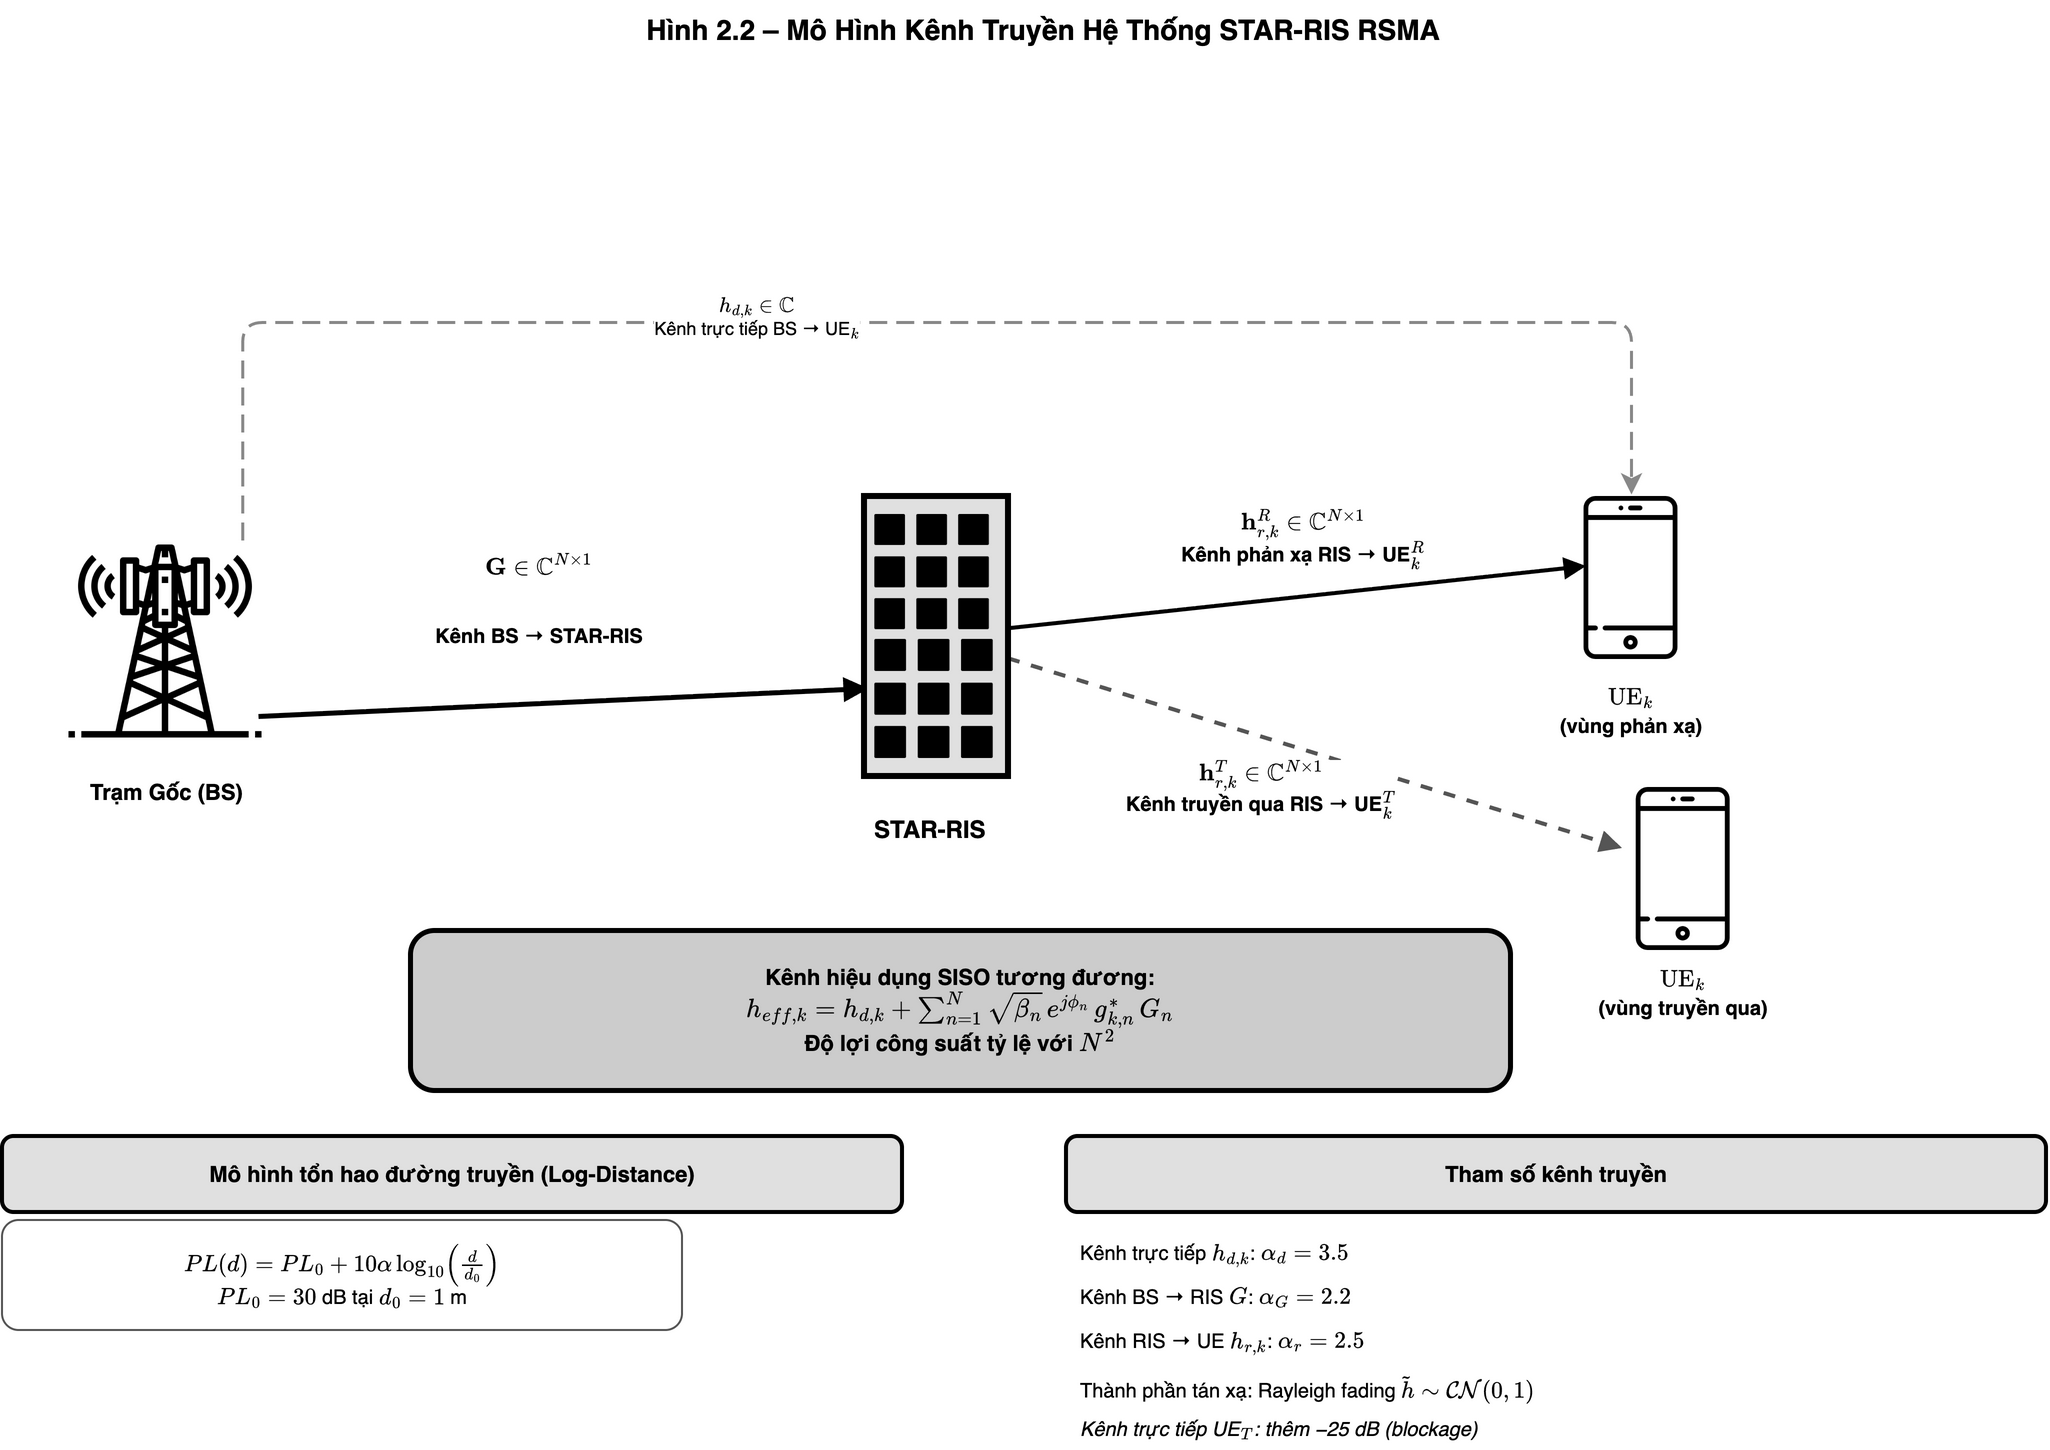
\includegraphics[width=0.96\linewidth]{figures/h2_2_kenh_truyen.png}
  \caption{Mô hình kênh truyền STAR-RIS RSMA: kênh trực tiếp $h_{d,k}$, kênh
  BS$\to$RIS $\mathbf{G}$, và kênh RIS$\to$UE $\mathbf{h}_{r,k}$ (cho cả hai
  vùng R và T).}
  \label{fig:h2_2}
\end{figure}

\textbf{Kênh trực tiếp BS$\to$UE$_k$:} ký hiệu $h_{d,k} \in \mathbb{C}$,
tuân theo phân phối Rayleigh $\mathcal{CN}(0, \zeta_{d,k}^2)$ với
$\zeta_{d,k}^2$ là độ lợi suy hao đường truyền tuyến trực tiếp.

\textbf{Kênh BS$\to$STAR-RIS:} ký hiệu $\mathbf{G} \in \mathbb{C}^{N \times 1}$,
mỗi phần tử là một biến phức Rayleigh độc lập.

\textbf{Kênh RIS$\to$UE$_k$:} ký hiệu $\mathbf{h}_{r,k}^X \in \mathbb{C}^{N \times 1}$
với $X \in \{R, T\}$ chỉ rõ vùng (phản xạ hay truyền qua).

\subsection{Mô hình suy hao đường truyền}

Suy hao đường truyền giữa hai điểm cách nhau $d$ mét tuân theo mô hình
log-distance \cite{wu2020smart}, \cite{mu2022simultaneously}:
\begin{equation}
  \mathrm{PL}(d) \;=\; \mathrm{PL}_0 + 10\,\alpha\,\log_{10}\!\frac{d}{d_0},
  \label{eq:pathloss}
\end{equation}
trong đó $\mathrm{PL}_0 = 30$ dB là suy hao tham chiếu tại $d_0=1$ m,
$\alpha$ là số mũ suy hao đường truyền. Các giá trị $\alpha$ khác nhau
cho từng loại kênh, được liệt kê trong Bảng \ref{tab:pathloss_param}.
Cụ thể, kênh trực tiếp BS$\to$UE có số mũ suy hao lớn nhất ($\alpha_d =
3{,}5$) phản ánh môi trường truyền sóng phức tạp, trong khi kênh
BS$\to$STAR-RIS được giả định gần đường truyền thẳng ($\alpha_G = 2{,}2$)
do thiết kế triển khai BS và RIS có tầm nhìn trực tiếp.

\begin{table}[t]
\centering
\caption{Số mũ suy hao đường truyền theo từng loại kênh.}
\label{tab:pathloss_param}
\begin{tabular}{p{6cm} c c}
\toprule
\textbf{Kênh} & \textbf{Ký hiệu} & \textbf{$\alpha$} \\
\midrule
Kênh trực tiếp BS$\to$UE                & $h_{d,k}$              & $3{,}5$ \\
Kênh BS$\to$STAR-RIS                    & $\mathbf{G}$           & $2{,}2$ \\
Kênh STAR-RIS$\to$UE                    & $\mathbf{h}_{r,k}$     & $2{,}5$ \\
\bottomrule
\end{tabular}
\end{table}

Kênh trực tiếp tới người dùng vùng T chịu thêm suy hao chướng ngại
$-25$ dB nhằm mô phỏng trường hợp NLoS, lý do STAR-RIS được triển khai.

\subsection{Hệ số phản xạ và truyền qua của STAR-RIS}
\label{sec:star_ris_coef}

Theo mục \ref{sec:starris} của Chương 1, mỗi phần tử thứ $n$ của
STAR-RIS có các hệ số phản xạ $\Phi_n^R$ và truyền qua $\Phi_n^T$ định
nghĩa trong \eqref{eq:starris_coef}.

\textbf{Quy ước về $\beta_n^X$:} Trong toàn bộ Luận văn này, đại lượng
$\beta_n^X \in [0,1]$ được định nghĩa là hệ số phân chia năng lượng
(power-splitting coefficient) tại phần tử $n$ trong vùng
$X \in \{R, T\}$, \textbf{không phải là biên độ}. Cụ thể:
\begin{equation}
|\Phi_n^X|^2 \;=\; \beta_n^X, \qquad
\Phi_n^X \;=\; \sqrt{\beta_n^X}\,e^{j\theta_n^X},
\label{eq:beta_def}
\end{equation}
nghĩa là $\sqrt{\beta_n^X}$ là biên độ phức của hệ số STAR-RIS, còn
$\beta_n^X$ là tỷ phần năng lượng tín hiệu được phân về vùng $X$. Với
quy ước này, định luật bảo toàn năng lượng STAR-RIS ở chế độ ES có
dạng tuyến tính theo $\beta$:
\begin{equation}
|\Phi_n^R|^2 + |\Phi_n^T|^2 \;=\; \beta_n^R + \beta_n^T \;=\; 1,
\quad \forall n \in \{1,\ldots,N\}.
\label{eq:es_constraint_full}
\end{equation}
Đây là dạng được sử dụng phổ biến trong các công trình STAR-RIS
\cite{liu2021starris}, \cite{mu2022simultaneously}. Hai ma trận pha dịch tổng
thể là:
\begin{align}
  \boldsymbol{\Phi}_R &= \mathrm{diag}\!\big(\sqrt{\beta_1^R}\,e^{j\theta_1^R},\,
  \ldots,\, \sqrt{\beta_N^R}\,e^{j\theta_N^R}\big), \label{eq:Phi_R}\\
  \boldsymbol{\Phi}_T &= \mathrm{diag}\!\big(\sqrt{\beta_1^T}\,e^{j\theta_1^T},\,
  \ldots,\, \sqrt{\beta_N^T}\,e^{j\theta_N^T}\big). \label{eq:Phi_T}
\end{align}

\textbf{Liên hệ giữa lý thuyết và cài đặt mô phỏng:} trong khuôn khổ
MADDPG ở Chương \ref{ch:chuong3}, tác tử RIS-R xuất trực tiếp giá trị
$\beta_n^R \in [0,1]$ (qua biến đổi affine $\beta_n^R = 0{,}5(a_n + 1)$
từ đầu ra $\tanh$). Giá trị $\beta_n^T$ được suy ra theo
\eqref{eq:es_constraint_full} là $\beta_n^T = 1 - \beta_n^R$, đảm bảo
bảo toàn năng lượng tự động ở mọi bước. Đây là lý do tác giả
chọn quy ước $\beta$ là hệ số năng lượng (chứ không phải biên độ): cách
chọn này cho phép ràng buộc tuyến tính đơn giản, tránh phải thực thi
ràng buộc bậc hai $\sqrt{\beta_n^R}^2 + \sqrt{\beta_n^T}^2 = 1$ phức tạp
hơn cho mạng nơ-ron.

\begin{figure}[t]
  \centering
  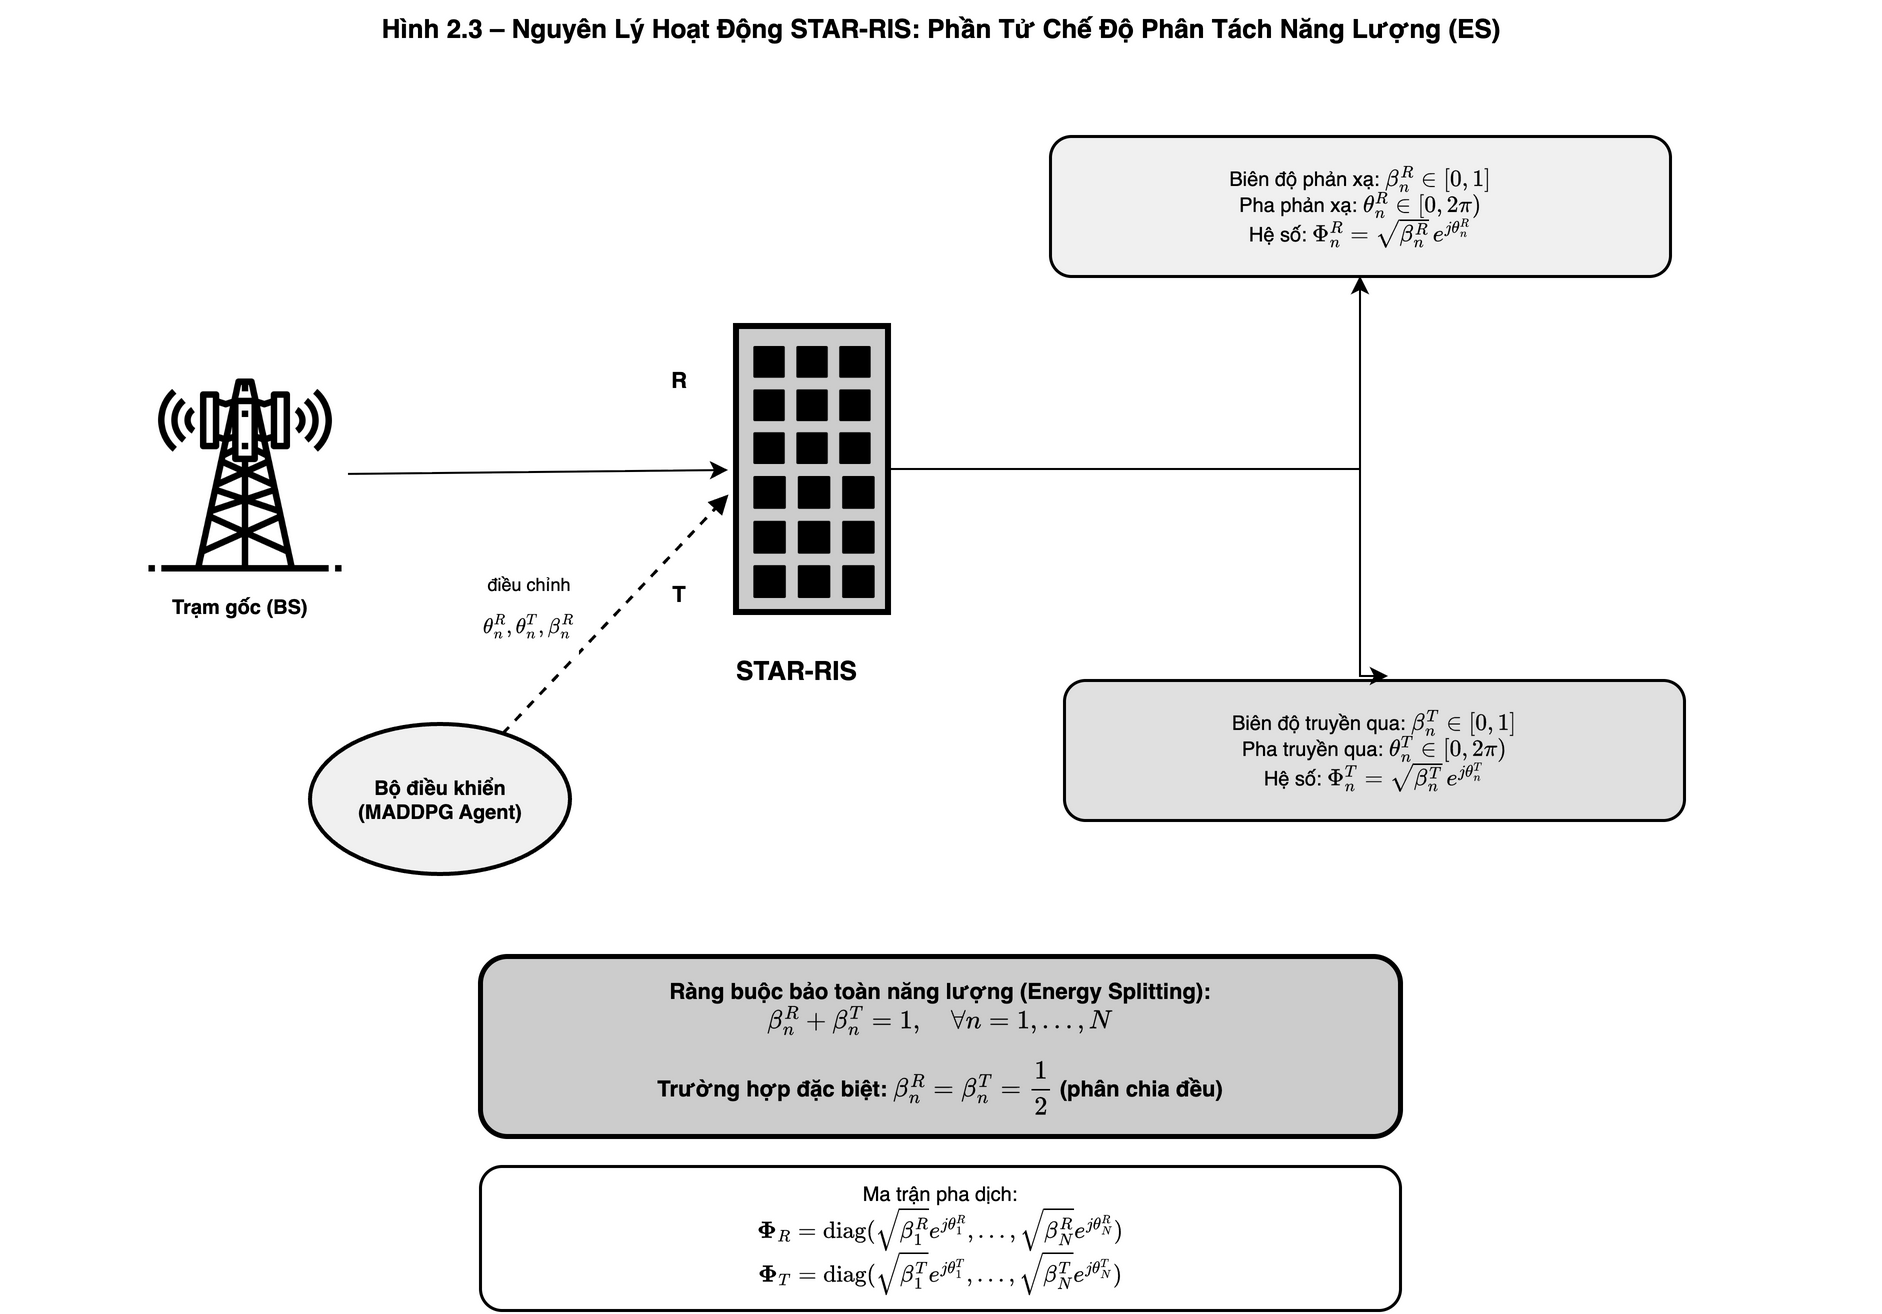
\includegraphics[width=0.92\linewidth]{figures/h2_3_star_ris_es.png}
  \caption{Nguyên lý hoạt động của phần tử STAR-RIS ở chế độ ES: sóng tới
  được phân tách thành sóng phản xạ (hệ số năng lượng $\beta_n^R$, pha
  $\theta_n^R$) và sóng truyền qua ($\beta_n^T$, $\theta_n^T$), thỏa
  $\beta_n^R + \beta_n^T = 1$.}
  \label{fig:h2_3}
\end{figure}

\subsection{Kênh hiệu dụng SISO tương đương}

Bằng cách gộp đường trực tiếp và đường gián tiếp qua STAR-RIS, ta thu
được kênh hiệu dụng SISO tương đương giữa BS và người dùng $k$
\cite{mao2022rsma}, \cite{hua2023learning}:
\begin{equation}
  h_{\text{eff},k} \;=\; h_{d,k} + \big(\mathbf{h}_{r,k}^X\big)^{\!H}\,
  \boldsymbol{\Phi}_X\,\mathbf{G}, \quad X \in \{R, T\},
  \label{eq:heff}
\end{equation}
hay tương đương dưới dạng tổng phần tử:
\begin{equation}
  h_{\text{eff},k} \;=\; h_{d,k} + \sum_{n=1}^{N} \sqrt{\beta_n^X}\,
  e^{j\theta_n^X}\, \big(\mathbf{h}_{r,k}^X\big)_n^*\,(\mathbf{G})_n.
  \label{eq:heff_sum}
\end{equation}
Hệ thức \eqref{eq:heff_sum} cho thấy rõ vai trò của STAR-RIS: bằng việc
chọn $\theta_n^X$ thích hợp, các pha của thành phần
$(\mathbf{h}_{r,k}^X)_n^*(\mathbf{G})_n$ có thể được căn chỉnh đồng
pha với $h_{d,k}$ để tối đa $|h_{\text{eff},k}|^2$. Khi $\theta_n^X$ được
chọn lý tưởng, độ lợi công suất kênh hiệu dụng tỷ lệ với $N^2$, nghĩa là
gấp đôi số phần tử RIS sẽ làm tăng độ lợi gấp bốn, một trong
những lý do khiến RIS được coi là công nghệ then chốt cho 6G.

% -----------------------------------------------------------------------------
\section{Mô hình tín hiệu RSMA, SINR và tốc độ đạt được}
\label{sec:rsma_signal}

\subsection{Tín hiệu phát và tín hiệu thu}

Theo công thức \eqref{eq:rsma_signal}, tín hiệu phát hợp nhất tại BS là
$x = \sqrt{P_c}\,s_c + \sum_{k=1}^{K}\sqrt{P_k}\,s_k$. Tín hiệu thu tại
người dùng $k$ qua kênh hiệu dụng là:
\begin{equation}
  y_k \;=\; h_{\text{eff},k}\,x + n_k
        \;=\; h_{\text{eff},k}\Big(\sqrt{P_c}\,s_c + \sum_{j=1}^{K}\sqrt{P_j}\,s_j\Big)
        + n_k,
  \label{eq:yk}
\end{equation}
với $n_k \sim \mathcal{CN}(0, \sigma^2)$ là tạp âm Gauss phức.

\subsection{Giải mã luồng chung và SINR luồng chung}

Người dùng $k$ trước tiên giải mã luồng chung $s_c$ trong khi xem các
luồng riêng (kể cả luồng riêng của chính mình) là nhiễu. SINR của luồng
chung tại UE $k$ là:
\begin{equation}
  \gamma_{c,k} \;=\; \frac{P_c\,|h_{\text{eff},k}|^2}
                          {\sum_{j=1}^{K} P_j\,|h_{\text{eff},k}|^2 + \sigma^2}.
  \label{eq:sinr_c}
\end{equation}
Tốc độ luồng chung mà UE $k$ có thể giải mã thành công là
$R_{c,k} = \log_2(1+\gamma_{c,k})$. Như đã giải thích trong Chương 1, vì
luồng chung phải được mọi người dùng giải mã, tốc độ luồng chung
khả thi bị giới hạn theo công thức $R_c = \min_k R_{c,k}$
\eqref{eq:rc_minmax}.

\subsection{Áp dụng SIC và SINR luồng riêng}

Sau khi giải mã thành công $\hat s_c$, UE $k$ trừ ảnh hưởng của nó khỏi
tín hiệu thu để có tín hiệu còn lại. SINR của luồng riêng của UE $k$
khi đó là:
\begin{equation}
  \gamma_{p,k} \;=\; \frac{P_k\,|h_{\text{eff},k}|^2}
                          {\sum_{j=1,\,j\neq k}^{K} P_j\,|h_{\text{eff},k}|^2 + \sigma^2}.
  \label{eq:sinr_p}
\end{equation}
Tốc độ luồng riêng là $R_{p,k} = \log_2(1+\gamma_{p,k})$.

\subsection{Tốc độ người dùng và tổng tốc độ hệ thống}

Theo định nghĩa của RSMA \cite{mao2022rsma}, tốc độ tổng mà UE $k$
nhận được là $R_k = c_k\,R_c + R_{p,k}$ \eqref{eq:rk}, và tổng tốc độ
toàn hệ thống là:
\begin{equation}
  R_{\text{sum}} \;=\; \sum_{k=1}^{K} R_k
                  \;=\; R_c + \sum_{k=1}^{K} R_{p,k},
  \label{eq:rsum}
\end{equation}
do $\sum_k c_k = 1$.

% -----------------------------------------------------------------------------
\section{Bài toán tối ưu (P0)}
\label{sec:P0}

\subsection{Phát biểu bài toán}

Mục tiêu của hệ thống là tối đa hóa tổng tốc độ $R_{\text{sum}}$ bằng
cách lựa chọn đồng thời ba nhóm biến tối ưu (xem Hình \ref{fig:h2_4}):
\begin{itemize}[leftmargin=*]
\item Vector công suất $\mathbf{P} = (P_c, P_1, P_2, \ldots, P_K)$;
\item Vector pha và biên độ STAR-RIS
$\boldsymbol{\Theta} = (\{\theta_n^R, \theta_n^T, \beta_n^R\}_{n=1}^{N})$
(do $\beta_n^T = 1 - \beta_n^R$ từ ràng buộc bảo toàn năng lượng);
\item Vector tỷ lệ tách $\mathbf{C} = (c_1, c_2, \ldots, c_K)$.
\end{itemize}

Hình \ref{fig:h2_4} biểu diễn cấu trúc tổng thể của bài toán P0, bao
gồm hàm mục tiêu max $R_{\text{sum}}$, ba nhóm biến tối ưu và sáu nhóm
ràng buộc về công suất, năng lượng, tỷ lệ tách, pha, biên độ và QoS.
Phần dưới của hình tóm tắt tính phi lồi của bài toán và động lực sử
dụng MADDPG để giải.

\begin{figure}[t]
  \centering
  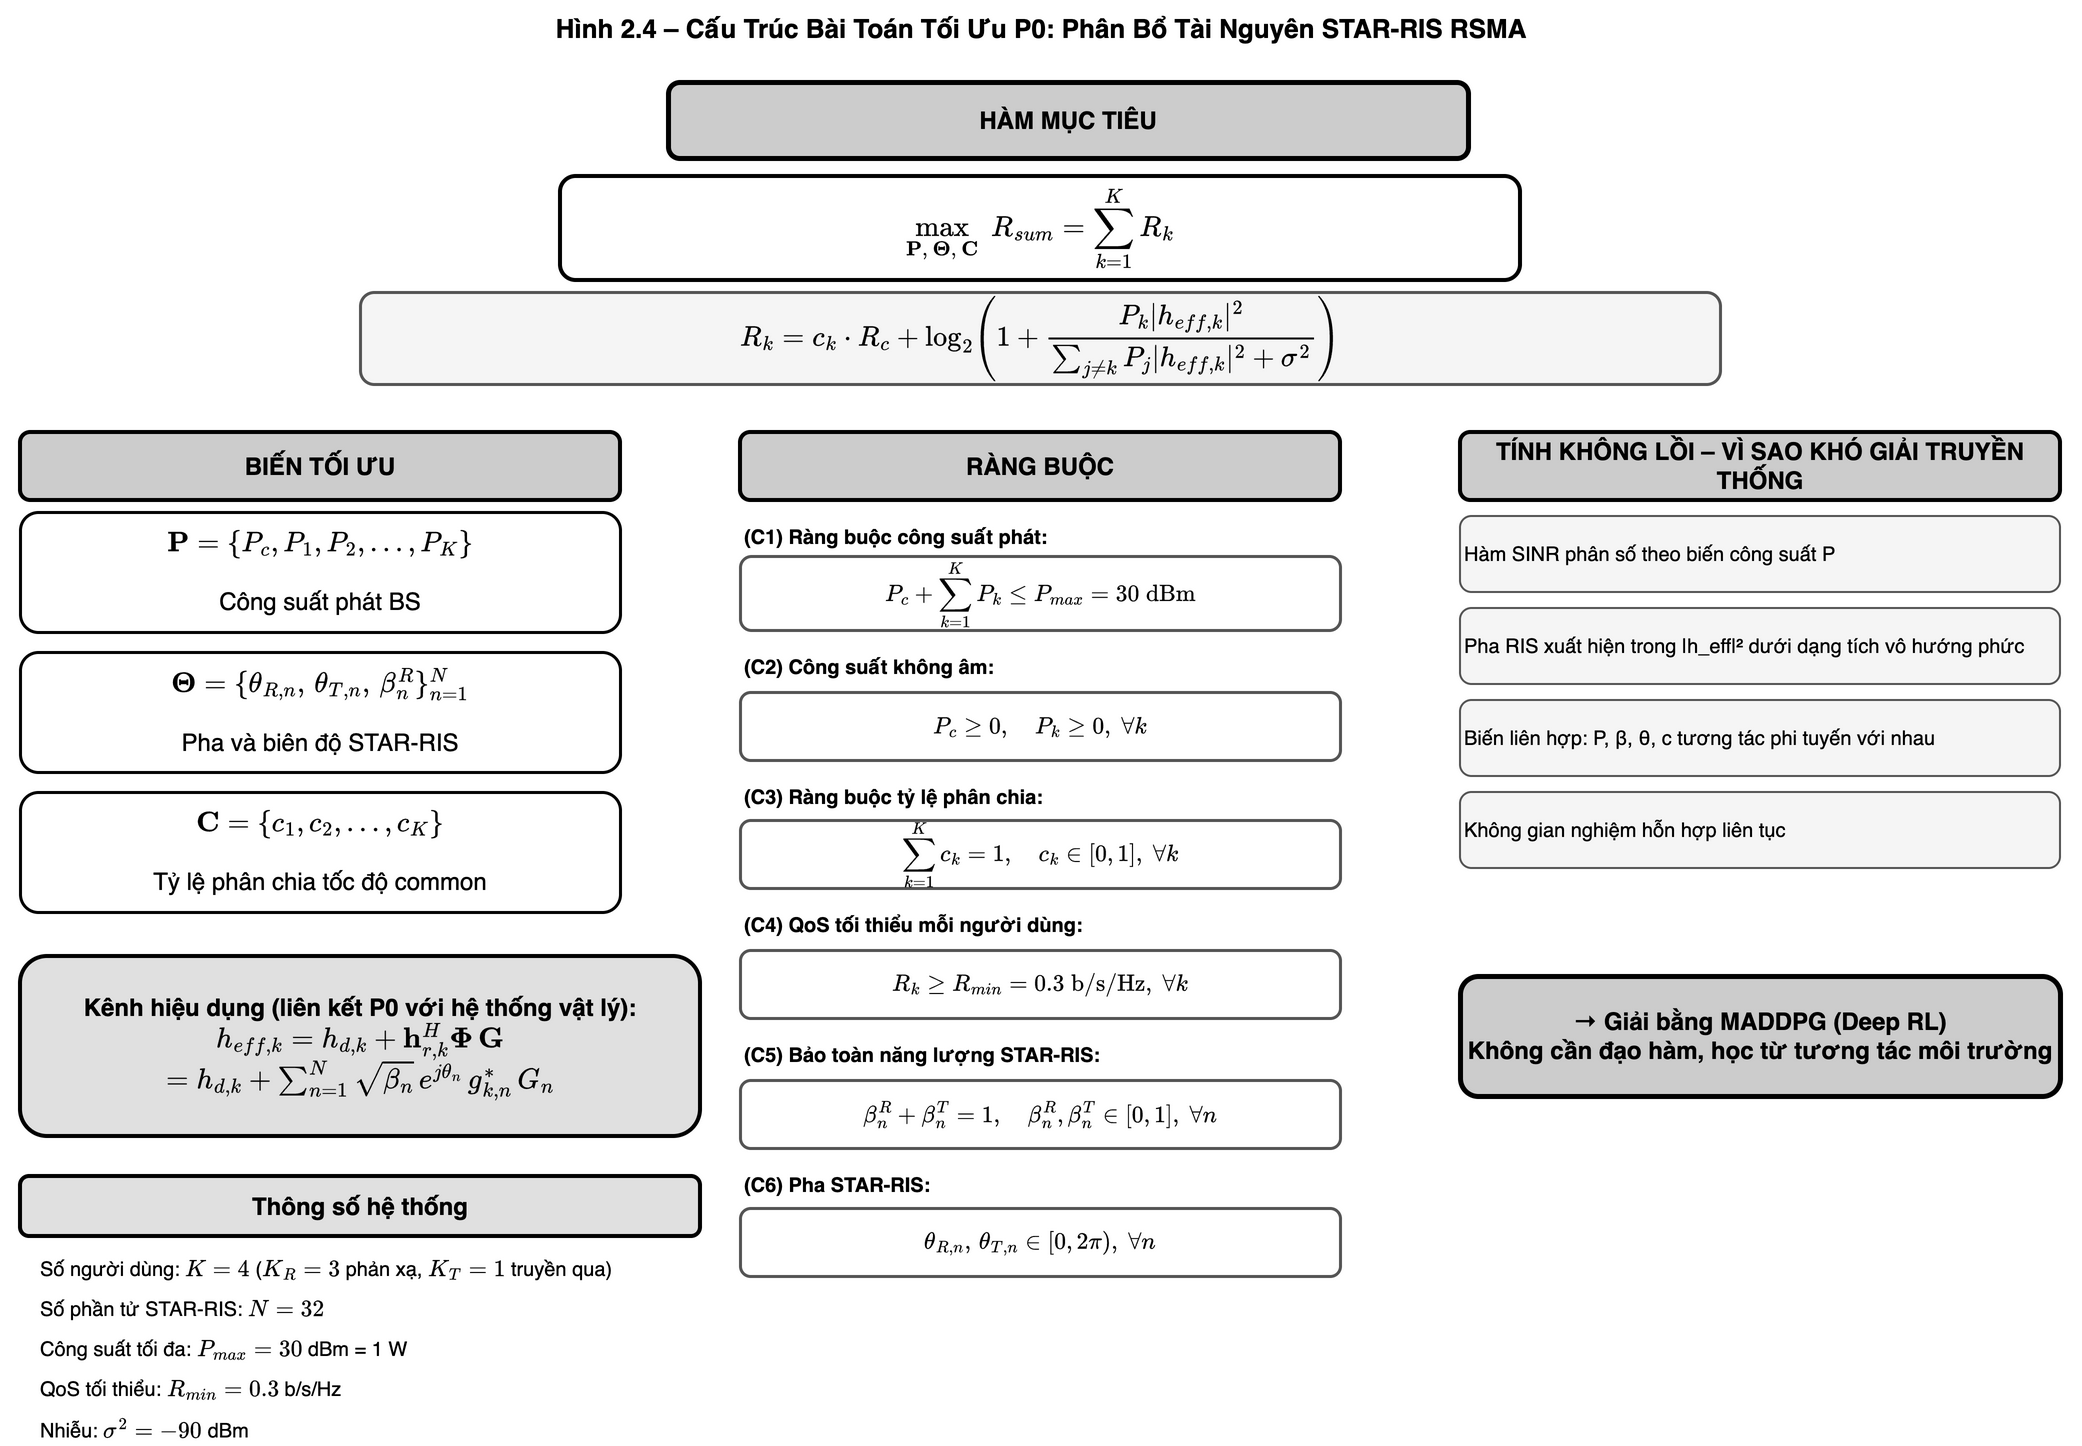
\includegraphics[width=0.95\linewidth]{figures/h2_4_bai_toan_p0.png}
  \caption{Cấu trúc bài toán tối ưu P0: hàm mục tiêu max $R_{\text{sum}}$,
  ba nhóm biến tối ưu và sáu nhóm ràng buộc.}
  \label{fig:h2_4}
\end{figure}

Bài toán tối ưu P0 được phát biểu như sau:

\begin{equation}
\begin{aligned}
(\text{P0}):\quad & \max_{\mathbf{P},\,\boldsymbol{\Theta},\,\mathbf{C}}
\; R_{\text{sum}} = \sum_{k=1}^{K} R_k \\[2pt]
\text{s.t.}\quad
& (\text{C1})\quad P_c + \sum_{k=1}^{K} P_k \;\leq\; P_{\max}, \\
& (\text{C2})\quad P_c \geq 0,\; P_k \geq 0,\; \forall k, \\
& (\text{C3})\quad \sum_{k=1}^{K} c_k = 1,\; c_k \in [0,1],\; \forall k, \\
& (\text{C4})\quad R_k \geq R_{\min},\; \forall k \in \{1,\ldots,K\}, \\
& (\text{C5})\quad \beta_n^R + \beta_n^T = 1,\;
                   \beta_n^R, \beta_n^T \in [0,1],\; \forall n, \\
& (\text{C6})\quad \theta_n^R, \theta_n^T \in [0, 2\pi),\; \forall n.
\end{aligned}
\label{eq:P0}
\end{equation}

Các ràng buộc có ý nghĩa: (C1)--(C2) đảm bảo công suất phát không vượt
$P_{\max}=30$~dBm; (C3) đảm bảo tổng tỷ lệ phân chia luồng chung bằng 1;
(C4) ràng buộc QoS yêu cầu mỗi UE đạt tốc độ tối thiểu
$R_{\min}=0{,}3$~b/s/Hz; (C5)--(C6) là các ràng buộc nội tại của STAR-RIS.

\textbf{Nhận xét quan trọng.} So với mô hình P0 cổ điển trong các nghiên
cứu trước \cite{mao2022rsma}, \cite{gomes2024performance}, bài toán P0 mà Luận
văn xem xét có hai điểm khác biệt: (i) ràng buộc QoS (C4) được thêm vào
một cách tường minh để phản ánh yêu cầu dịch vụ trong các kịch bản 6G
(khi giải bằng DRL, ràng buộc cứng này được xử lý qua một surrogate
ràng buộc mềm với cập nhật đối ngẫu, xem Mục \ref{sec:reward_surrogate});
và (ii) biên độ $\beta_n^R$ được xem là biến tối ưu thay
vì cố định ở giá trị $1/2$, qua đó cho phép phân phối năng lượng giữa hai
vùng linh hoạt hơn.

\subsection{Tính phi lồi và động lực sử dụng DRL}

Bài toán P0 \eqref{eq:P0} là một bài toán phi lồi rất khó giải vì nhiều
nguyên nhân kết hợp \cite{wu2020smart}, \cite{mao2022rsma}, \cite{irkicatal2024deep}:

\textbf{(i) Hàm SINR \eqref{eq:sinr_c} và \eqref{eq:sinr_p} là tỷ số phân
thức theo công suất.} Do đó hàm mục tiêu $R_{\text{sum}}$, là tổng các
$\log_2(1+\gamma)$, không lồi trên không gian công suất $\mathbf{P}$.

\textbf{(ii) Biến pha $\theta_n$ xuất hiện trong $h_{\text{eff},k}$ dưới
dạng hàm mũ phức $e^{j\theta_n}$.} Bình phương biên độ $|h_{\text{eff},k}|^2$
mở rộng thành tổng các tích chéo $\cos(\theta_n - \theta_m)$, không lồi
theo $\theta$.

\textbf{(iii) Tương tác phi tuyến giữa các nhóm biến.} $\mathbf{P}$,
$\boldsymbol{\Theta}$, $\mathbf{C}$ liên kết với nhau qua hàm mục tiêu và
ràng buộc QoS theo cách phi tuyến phức tạp.

\textbf{(iv) Ràng buộc QoS (C4) là phi lồi.} Tập khả thi $R_k \geq R_{\min}$
được định nghĩa qua các hàm $\log$ của tỷ số phi tuyến, không lồi.

Các phương pháp cổ điển (BCD, SDR, AO) tuy có thể tìm điểm dừng cục bộ
nhưng chi phí tính toán cao, không phù hợp cho cập nhật thời gian thực
trong các kịch bản 6G với kênh biến thiên ở mức ms. Hơn nữa, các phương
pháp này thường đòi hỏi hiểu biết chính xác về mô hình kênh, một giả
thiết không phải lúc nào cũng đúng trong thực tế. Vì vậy, Luận văn lựa
chọn hướng tiếp cận học tăng cường sâu để giải bài toán P0.

% -----------------------------------------------------------------------------
\section{Ánh xạ sang quá trình ra quyết định Markov}
\label{sec:mdp}

Để áp dụng DRL/MADDPG, bài toán P0 cần được ánh xạ sang một MDP với bộ năm
$(\mathcal{S}, \mathcal{A}, \mathcal{P}, \mathcal{R}, \gamma)$ phù hợp với
cơ chế ba tác tử chuyên dụng. Hình \ref{fig:h2_5} tóm lược ánh xạ MDP,
trong đó không gian trạng thái 550 chiều được phân thành ba phần tương
ứng quan sát cục bộ của từng tác tử, không gian hành động 105 chiều bao
gồm công suất, biên độ, pha và tỷ lệ tách, còn hàm phần thưởng là
Lagrangian surrogate giữa sum-rate và mức đáp ứng QoS. Bố cục chi tiết
của quan sát/hành động được sinh tự động từ mã nguồn qua
\texttt{observation\_schema()} / \texttt{action\_schema()}
(file \texttt{observation\_schema.json}), bảo đảm mô tả dưới đây khớp
tuyệt đối với cài đặt.

% LUU Y: hinh h2_5/h2_6 can ve lai theo so chieu moi (550/655) sau refactor.
\begin{figure}[t]
  \centering
  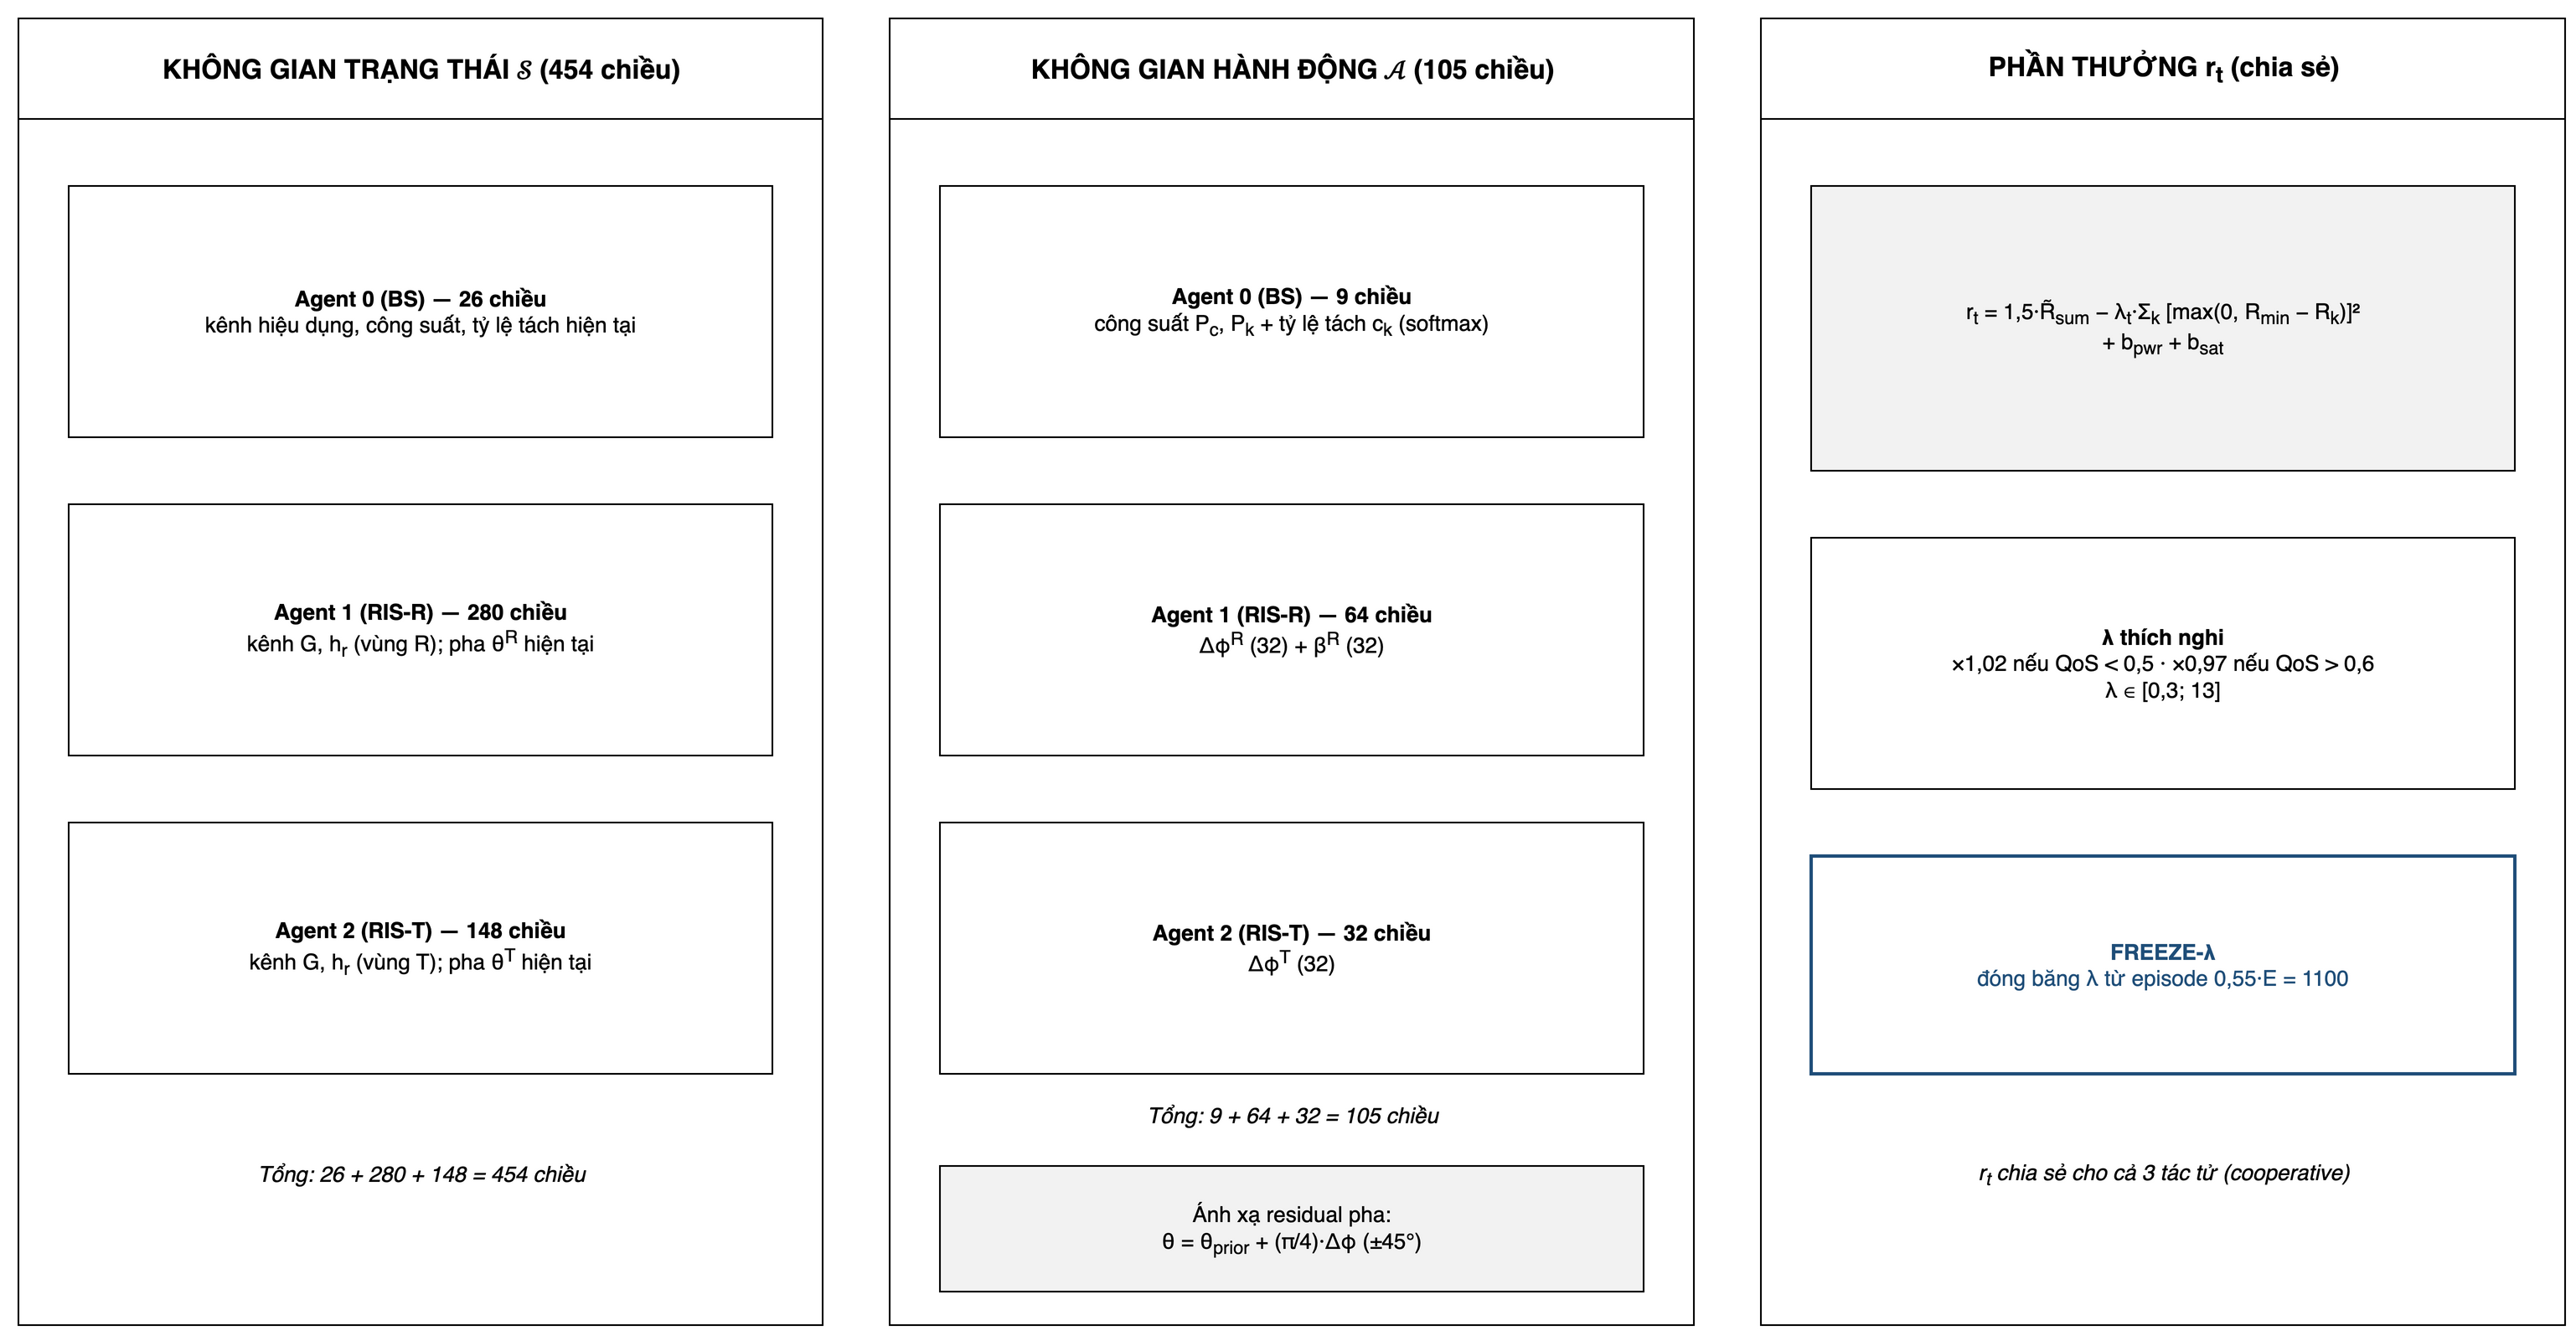
\includegraphics[width=0.96\linewidth]{figures/h2_5_mdp_anh_xa.png}
  \caption{Ánh xạ bài toán P0 sang MDP: không gian trạng thái 550 chiều
  (tổng quan sát cục bộ ba tác tử), không gian hành động 105 chiều,
  hàm phần thưởng Lagrangian surrogate với cập nhật đối ngẫu per-user.}
  \label{fig:h2_5}
\end{figure}

\subsection{Không gian trạng thái}

Trạng thái tổng thể $s_t$ là phép hợp các quan sát cục bộ của ba tác tử
$s_t = (o_{0,t}, o_{1,t}, o_{2,t})$, với tổng số chiều
$26 + 344 + 180 = 550$ (cấu hình chuẩn $K=4$, $K_R=3$, $N=32$). Mỗi quan
sát cục bộ bắt đầu bằng khối chung 18 chiều: phần thực và phần ảo của
kênh hiệu dụng $h_{\text{eff},k}$ (8), vector trọng số công suất softmax
ở bước trước (5), tỷ lệ tách ở bước trước (4) và phần thưởng bước trước
(1). Cụ thể:

\textbf{Tác tử BS (Agent 0, $o_0 \in \R^{26}$):} khối chung (18) cùng
phần thực/ảo của các kênh trực tiếp $h_{d,k}$ cho cả 4 UE (8).

\textbf{Tác tử STAR-RIS Reflection (Agent 1, $o_1 \in \R^{344}$):} khối
chung (18); phần thực/ảo của $h_{d,k}$ vùng R (6); của $\mathbf{G}$ (64);
của $\mathbf{h}_{r,k}^R$ với $k \in \{1,2,3\}$ (192); và trạng thái
STAR-RIS đang áp dụng: biên độ $\beta_n^R$ (32) cùng pha phản xạ hiện
hành $\phi_n^R$ (32).

\textbf{Tác tử STAR-RIS Transmission (Agent 2, $o_2 \in \R^{180}$):} khối
chung (18); phần thực/ảo của $h_{d,4}$ (2); của $\mathbf{G}$ (64); của
$\mathbf{h}_{r,4}^T$ (64); và 32 pha truyền qua hiện hành $\phi_n^T$.

Thành phần trạng thái STAR-RIS hiện hành là cần thiết cho tính Markov
của bài toán: chi phí tái cấu hình ở bước sau phụ thuộc cấu hình đang
áp dụng, nên cấu hình đó phải xuất hiện trong quan sát.

\subsection{Không gian hành động}

Tổng số chiều hành động là $9 + 64 + 32 = 105$:

\textbf{Tác tử BS (9 chiều):} 5 đại lượng cho công suất $\{P_c, P_1, \ldots,
P_K\}$ (qua softmax thành tỷ lệ rồi nhân với $P_{\max}$) và 4 đại lượng
cho tỷ lệ tách $\{c_1, \ldots, c_K\}$ (qua softmax để đảm bảo
$\sum c_k = 1$).

\textbf{Tác tử RIS-R (64 chiều), theo đúng thứ tự trong cài đặt:} 32 đại
lượng biên độ phản xạ $\{\beta_n^R\}_{n=1}^{N}$ (ánh xạ tuyến tính từ
$[-1,1]$ về $[0,1]$) đứng \emph{trước}, tiếp theo là 32 đại lượng phần dư
pha phản xạ $\{\Delta\phi_n^R\}_{n=1}^{N}$.

\textbf{Tác tử RIS-T (32 chiều):} 32 đại lượng phần dư pha truyền qua
$\{\Delta\phi_n^T\}_{n=1}^{N}$.

Tham số hóa pha kiểu residual (Chương 3 sẽ trình bày chi tiết):
\begin{equation}
\theta_n^X \;=\; \theta_n^{\text{prior},X} + \frac{\pi}{4}\,\Delta\phi_n^X,
\quad X \in \{R, T\},
\label{eq:residual_phase}
\end{equation}
giúp giảm khó khăn khám phá và tăng tốc hội tụ.

\subsection{Hàm phần thưởng: Lagrangian surrogate của P0}
\label{sec:reward_surrogate}

Ràng buộc QoS (C4) trong P0 là ràng buộc cứng. Trong khuôn khổ DRL, Luận
văn giải một bài toán \emph{surrogate} dạng phạt/Lagrangian của P0: ràng
buộc cứng được thay bằng ràng buộc kỳ vọng
$\mathbb{E}[c_k] \leq 0$ với hàm ràng buộc có dấu
$c_k = R_{\min} - R_k$ (tương đương $\mathbb{E}[R_k] \geq R_{\min}$).
Cách tiếp cận này \emph{không} bảo đảm QoS tại từng bước cho từng người
dùng; nó tối ưu điểm cân bằng throughput--QoS. Hàm phần thưởng:
\begin{equation}
\boxed{
r_t \;=\; \alpha\,\tilde R_{\text{sum}}
       \;-\; \sum_{k=1}^{K} \lambda_k\, c_{k,t}
       \;-\; \frac{w}{2} \sum_{k=1}^{K} \big[\max(0,\, c_{k,t})\big]^2
       \;-\; \eta_{\phi} C^{\phi}_t - \eta_{P} C^{P}_t - \eta_{\beta} C^{\beta}_t
}
\label{eq:reward}
\end{equation}
trong đó:
\begin{itemize}[leftmargin=*]
\item $\tilde R_{\text{sum}} = R_{\text{sum}}/R_{\text{ref}}$ là tổng tốc
độ chuẩn hóa theo tham chiếu $R_{\text{ref}}$ (tham số cấu hình
\texttt{reward\_rate\_reference}, giá trị $20$ b/s/Hz cho $K=4$);
$\alpha=1{,}5$;
\item $\lambda_k \geq 0$ là biến đối ngẫu riêng của từng người dùng, được
cập nhật bằng gradient đối ngẫu có phép chiếu trên trung bình episode
của chính $c_k$ (chi tiết ở Chương 3); số hạng bậc nhất dùng $c_k$
\emph{có dấu} như trong Lagrangian chuẩn;
\item $w$ là trọng số phạt bậc hai tăng cường (augmented penalty,
\texttt{augmented\_penalty\_weight}), chỉ tác dụng lên phần vi phạm
$\max(0, c_k)$;
\item $C^{\phi}_t, C^{P}_t, C^{\beta}_t$ là chi phí tái cấu hình pha,
công suất và biên độ so với hành động đã áp ở bước trước (chuẩn hóa
theo số chiều; bằng $0$ tại $t=0$), với các trọng số
$\eta_{\phi}, \eta_{P}, \eta_{\beta}$.
\end{itemize}
Hai chỉ số QoS được báo cáo tách bạch trong toàn bộ Luận văn:
\begin{align}
\text{user\_qos\_fraction} &= \frac{1}{K}\sum_{k=1}^{K}
\mathbf{1}\!\left[R_k \geq R_{\min}\right]
\quad\text{(tỷ lệ người dùng đạt QoS)},
\label{eq:user_qos_fraction}\\
\text{all\_users\_qos} &= \mathbf{1}\!\left[\min_k R_k \geq R_{\min}\right]
\quad\text{(tất cả người dùng đồng thời đạt QoS)}.
\label{eq:all_users_qos}
\end{align}
Đây là hai đại lượng khác nhau; mỗi bảng/hình đều ghi rõ metric nào
được dùng.

\subsection{Phân rã ba tác tử}

Hình \ref{fig:h2_6} biểu diễn phân rã ba tác tử chuyên dụng với chi tiết
các kích thước quan sát/hành động và kiến trúc Critic tập trung. Chi tiết
kiến trúc mạng và quy trình huấn luyện sẽ được trình bày trong Chương 3.

\begin{figure}[t]
  \centering
  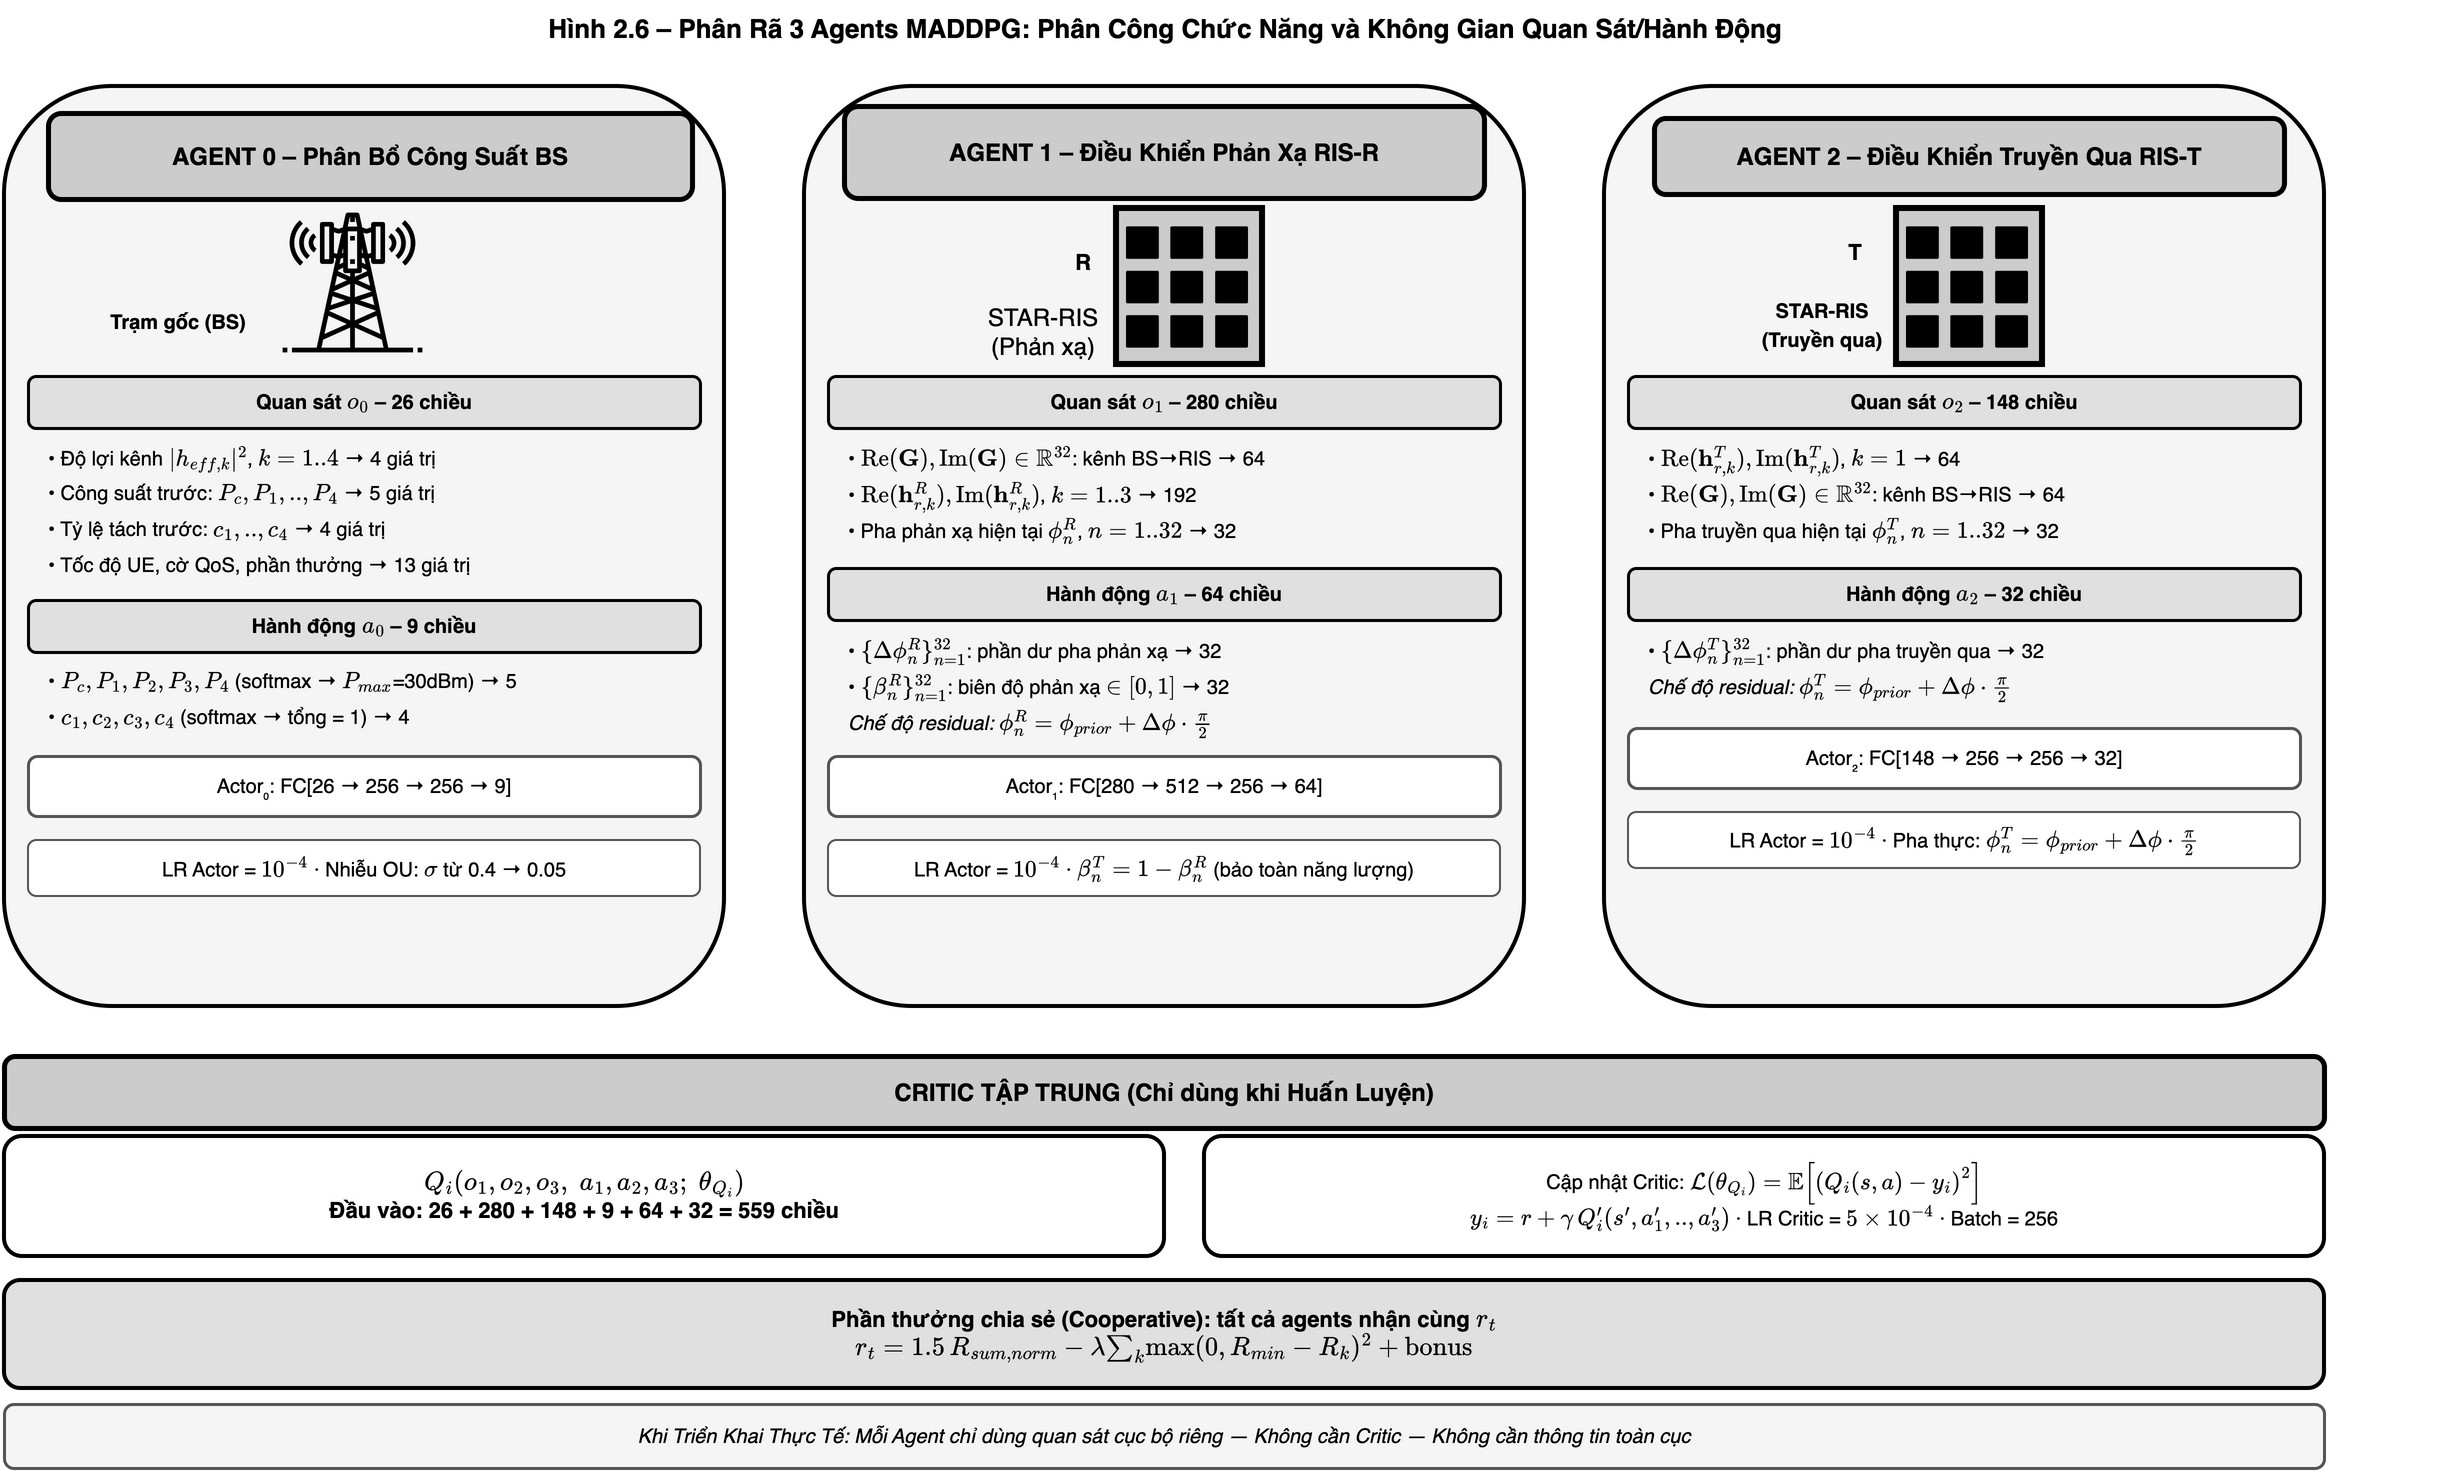
\includegraphics[width=0.96\linewidth]{figures/h2_6_3agents.png}
  \caption{Phân rã ba tác tử chuyên dụng: BS Power Agent ($26 \to 9$),
  RIS-R Agent ($344 \to 64$), RIS-T Agent ($180 \to 32$), và Critic tập
  trung với đầu vào $550 + 105 = 655$ chiều.}
  \label{fig:h2_6}
\end{figure}

% -----------------------------------------------------------------------------
\section{Tổng quan luồng hoạt động hệ thống}
\label{sec:overall_workflow}

Để định vị rõ ràng vai trò của khuôn khổ MADDPG đề xuất trong toàn bộ
hệ thống, Hình \ref{fig:overall_workflow} biểu diễn sơ đồ tổng quan
luồng hoạt động từ đầu cuối, gồm hai lớp được phân tách trực quan: lớp
vật lý (Physical Transmission Layer) chứa các khối truyền-nhận và lớp
điều khiển (MADDPG Controller) chứa các tác tử học.

\begin{figure}[t]
  \centering
  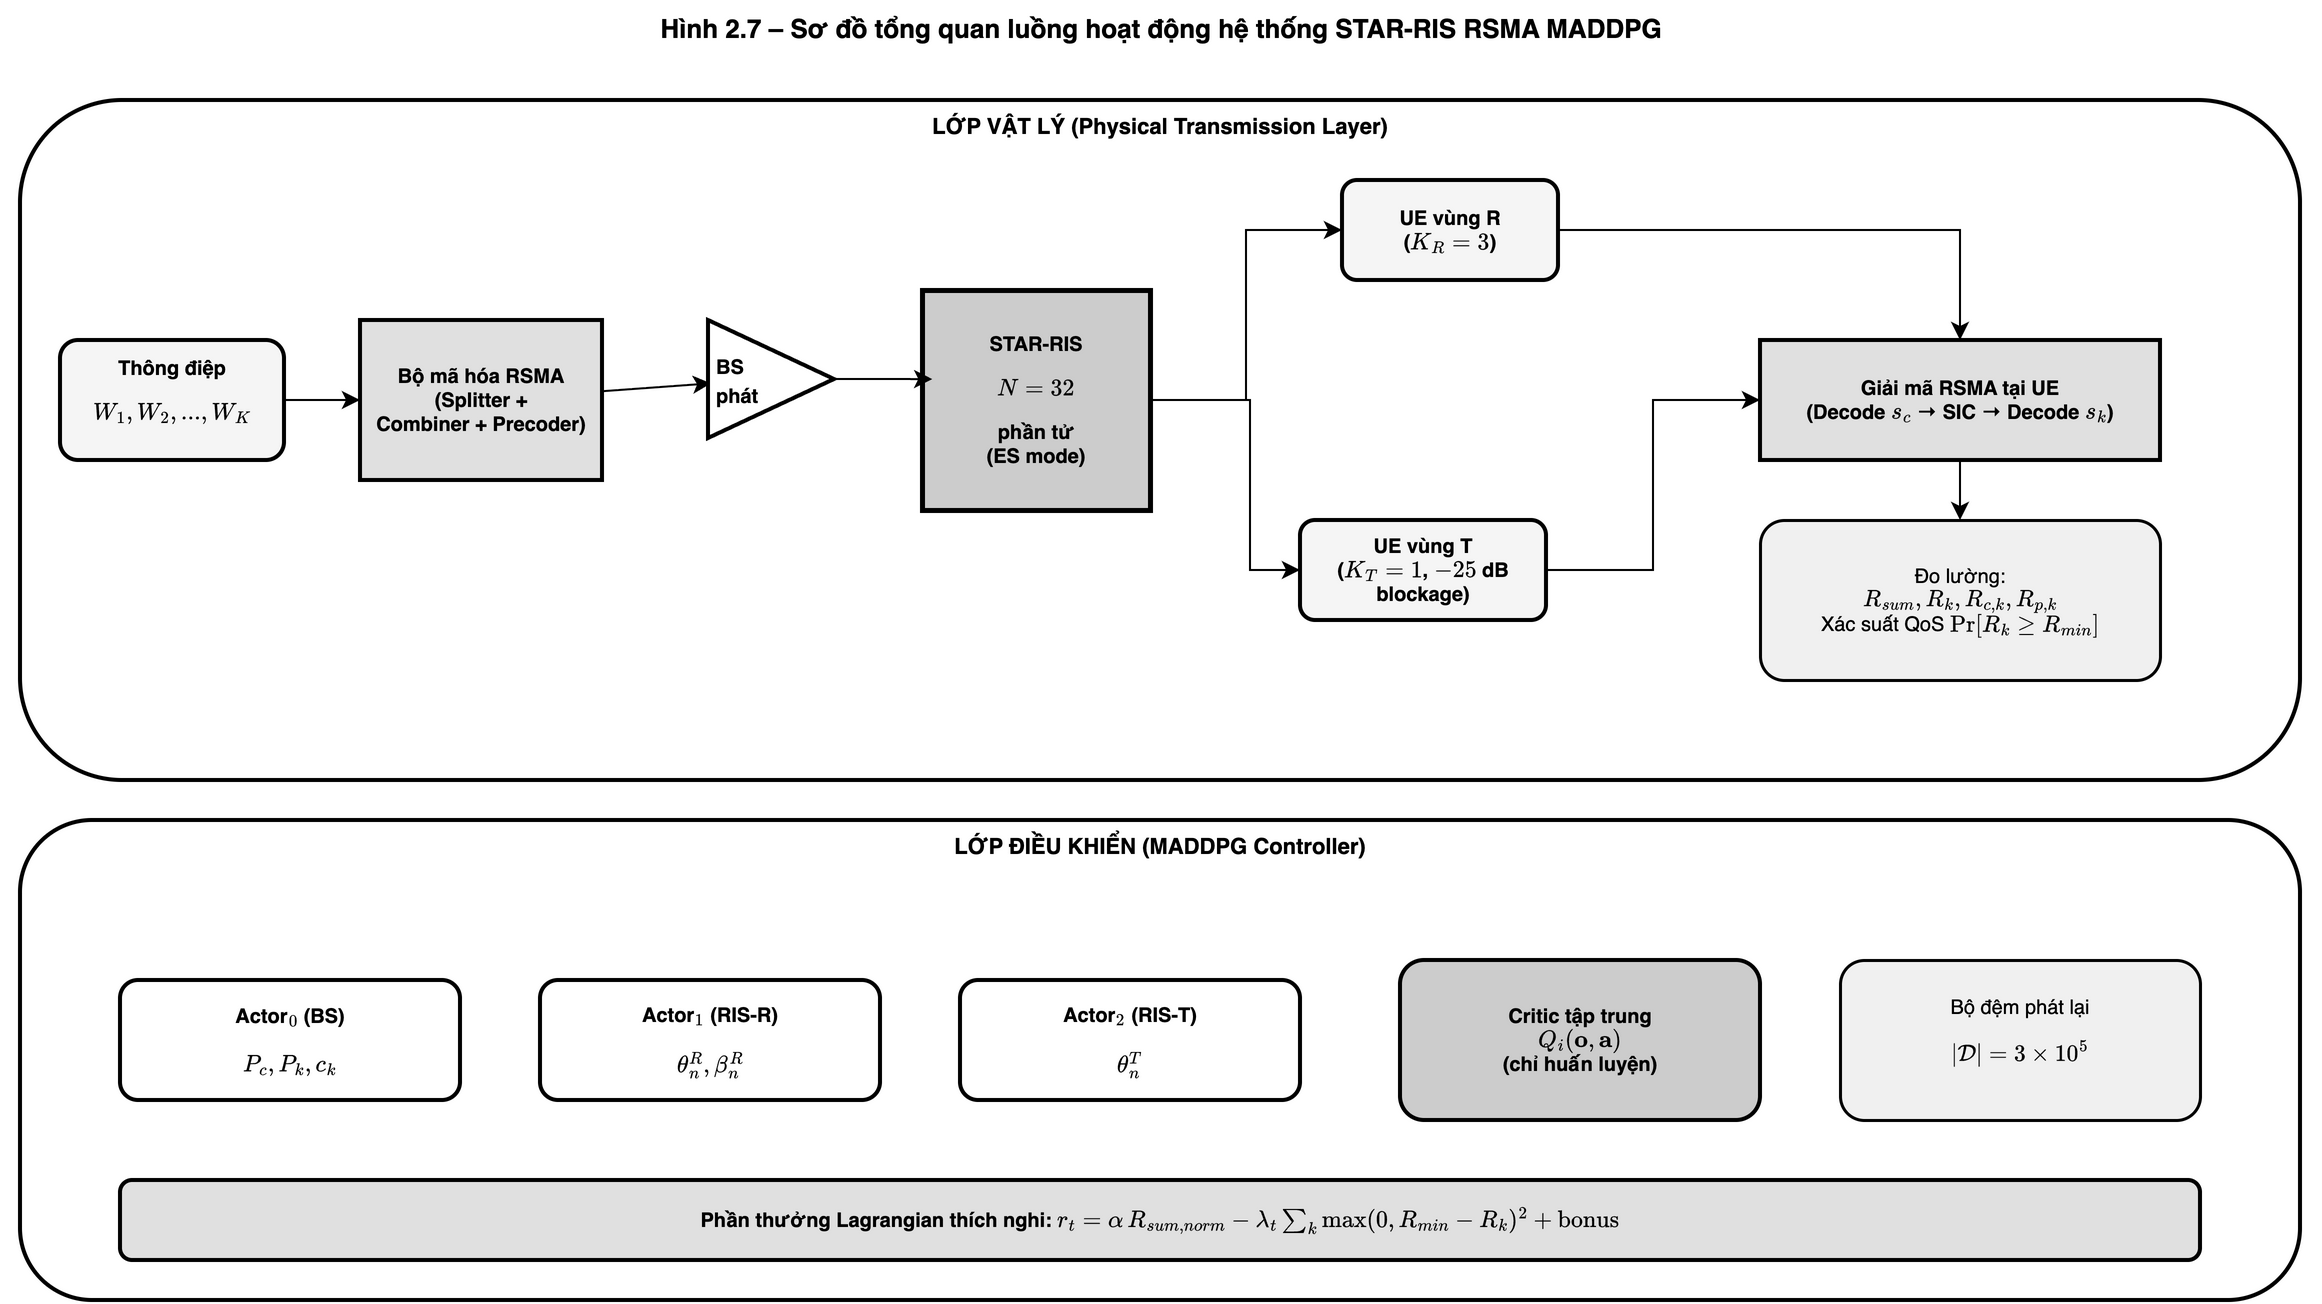
\includegraphics[width=0.98\linewidth]{figures/h2_7_overall_workflow.png}
  \caption{Sơ đồ tổng quan luồng hoạt động hệ thống STAR-RIS RSMA
  MADDPG. Lớp vật lý gồm bộ mã hóa RSMA, BS, STAR-RIS, các UE và các
  khối SIC, giải mã. Lớp điều khiển gồm ba tác tử Actor và Critic tập
  trung (chỉ dùng khi huấn luyện), được điều khiển bởi phần thưởng
  Lagrangian thích nghi.}
  \label{fig:overall_workflow}
\end{figure}

Luồng hoạt động end-to-end diễn ra như sau. Tại BS, thông điệp gốc
$\{W_k\}_{k=1}^K$ được bộ mã hóa RSMA tách thành luồng chung $s_c$ và
các luồng riêng $s_k$, sau đó kết hợp thành tín hiệu phát $x$ theo
\eqref{eq:rsma_signal}. Tín hiệu này được phát qua kênh trực tiếp
$h_{d,k}$ và đồng thời được điều hướng bởi STAR-RIS với hai ma trận
$\boldsymbol{\Phi}_R$ và $\boldsymbol{\Phi}_T$ tác động lên các vùng
phản xạ và truyền qua. Tại mỗi UE, quá trình giải mã RSMA gồm hai bước
nối tiếp: giải mã luồng chung, áp dụng SIC, sau đó giải mã luồng riêng.
Sum-rate và mức đáp ứng QoS đo được tại các UE được sử dụng làm tín
hiệu phản hồi (feedback) để tính phần thưởng $r_t$, từ đó cập nhật các
mạng Actor và Critic. Trong khi huấn luyện, Critic tập trung sử dụng
toàn bộ quan sát và hành động ghép $(\mathbf{o}, \mathbf{a})$ thông
qua các mẫu trong bộ đệm phát lại $\mathcal{D}$. Khi triển khai thực
tế, Critic được bỏ đi, chỉ ba Actor được giữ lại để sinh hành động
$\{a_{i,t}\}_{i=0,1,2}$ một cách phi tập trung dựa trên quan sát cục
bộ $o_{i,t}$.

% -----------------------------------------------------------------------------
\section*{Kết luận chương}
\addcontentsline{toc}{section}{Kết luận chương}

Chương 2 đã xây dựng đầy đủ mô hình hệ thống STAR-RIS hỗ trợ RSMA với
các thành phần BS-RIS-UE, mô hình kênh truyền (suy hao log-distance,
pha-đinh Rayleigh, chướng ngại $-25$~dB cho vùng T), và mô hình tín hiệu
RSMA với SINR và tốc độ. Bài toán tối ưu phân bổ tài nguyên P0
\eqref{eq:P0} được phát biểu với hàm mục tiêu max $R_{\text{sum}}$ và sáu
nhóm ràng buộc, đặc biệt bổ sung ràng buộc QoS trên từng người dùng.
Sau đó bài toán được ánh xạ sang MDP với ba tác tử chuyên dụng, không gian
trạng thái 550 chiều, không gian hành động 105 chiều và hàm phần thưởng
Lagrangian thích nghi. Chương 3 sẽ trình bày thiết kế chi tiết của khuôn
khổ MADDPG để giải MDP này.


% Chương 3
% =============================================================================
%  CHƯƠNG 3 – PHƯƠNG PHÁP ĐỀ XUẤT MADDPG
% =============================================================================
\chapter{PHƯƠNG PHÁP ĐỀ XUẤT MADDPG}
\label{ch:chuong3}

Chương này trình bày chi tiết phương pháp đề xuất của Luận văn để giải
bài toán surrogate của P0 \eqref{eq:P0}: Khuôn khổ MADDPG ba tác tử
chuyên dụng với cơ chế CTDE, kèm theo ba cải tiến chính: (i) tham số
hóa pha residual dựa trên nghiệm phân tích bậc một; (ii) hàm phần
thưởng Lagrangian surrogate với các biến đối ngẫu $\lambda_k$ per-user
cập nhật bằng projected dual gradient; và (iii) lịch trình heuristic
hai pha (two-stage dual freeze) giúp phần thưởng trở nên dừng
(stationary) ở giai đoạn cuối huấn luyện, nhờ đó đường cong huấn luyện
dễ diễn giải.

% -----------------------------------------------------------------------------
\section{Tổng quan kiến trúc MADDPG-CTDE đề xuất}
\label{sec:maddpg_overview}

\subsection{Sơ đồ tổng thể}

Như đã trình bày ở mục \ref{sec:maddpg} của Chương 1, MADDPG sử dụng cơ
chế huấn luyện tập trung, thực thi phân tán (CTDE)
\cite{lowe2017multi}. Trong giai đoạn huấn luyện, mỗi tác tử có một
Actor cục bộ và chia sẻ một Critic tập trung, vì vậy Critic luôn quan
sát đầy đủ trạng thái và hành động của toàn hệ thống, đảm bảo môi trường
ổn định từ góc nhìn của Critic. Trong giai đoạn thực thi, Critic được bỏ
đi; mỗi Actor chỉ cần quan sát cục bộ để sinh hành động.

Khuôn khổ MADDPG đề xuất trong Luận văn được thiết kế đặc thù cho bài
toán P0 với ba tác tử chuyên dụng:
\begin{itemize}[leftmargin=*]
\item \textbf{Tác tử 0, BS Power Agent:} điều khiển phân bổ công suất
$\{P_c, P_1, \ldots, P_K\}$ và tỷ lệ tách $\{c_1, \ldots, c_K\}$.
\item \textbf{Tác tử 1, STAR-RIS Reflection Agent:} điều khiển pha
$\{\theta_n^R\}$ và biên độ $\{\beta_n^R\}$ phản xạ.
\item \textbf{Tác tử 2, STAR-RIS Transmission Agent:} điều khiển pha
$\{\theta_n^T\}$ truyền qua (biên độ $\beta_n^T = 1 - \beta_n^R$ được
suy ra từ ràng buộc bảo toàn năng lượng).
\end{itemize}

\subsection{Lý do phân rã thành ba tác tử chuyên dụng}

So với cách triển khai một tác tử duy nhất với không gian hành động hợp
nhất 140 chiều, hoặc cách triển khai $N$ tác tử (mỗi phần tử RIS một tác
tử), khuôn khổ ba tác tử chuyên dụng có ba ưu điểm
\cite{lowe2017multi}, \cite{dange2026collaborative}, \cite{mirza2024multi}:

\textbf{(i) Mỗi tác tử có vai trò chức năng rõ ràng,} dễ phân tích và gỡ
lỗi. Tác tử BS chỉ tập trung vào tài nguyên thời gian-công suất, các tác
tử STAR-RIS chỉ tập trung vào tài nguyên không gian (pha-biên độ).

\textbf{(ii) Không gian hành động của mỗi tác tử nhỏ vừa phải,} dễ huấn
luyện hơn so với một tác tử 140 chiều. Đồng thời, số tác tử vừa đủ
(3) để Critic tập trung không gặp vấn đề chiều cao.

\textbf{(iii) Tách biệt được thông tin quan sát.} Tác tử BS không cần
biết chi tiết kênh BS-RIS-UE; tác tử RIS-R không cần biết tốc độ tổng
hiện tại. Điều này giảm chiều quan sát của từng tác tử, đẩy nhanh học.

% -----------------------------------------------------------------------------
\section{Kiến trúc mạng nơ-ron}
\label{sec:nn_architecture}

\subsection{Mạng Actor}

Mỗi tác tử $i \in \{0, 1, 2\}$ có một mạng Actor
$\mu_i: \R^{|o_i|} \to \R^{|a_i|}$ với kiến trúc multi-layer
perceptron (MLP) ba lớp \cite{lillicrap2016continuous}:
\begin{equation}
\mu_i(o_i) = \tanh\!\big(W^{(3)}_i\,\sigma(\mathrm{LN}(W^{(2)}_i\,
            \sigma(\mathrm{LN}(W^{(1)}_i\,o_i + b^{(1)}_i)) + b^{(2)}_i))
            + b^{(3)}_i\big),
\label{eq:actor_nn}
\end{equation}
trong đó $\sigma(\cdot) = \mathrm{ReLU}(\cdot)$ là hàm kích hoạt phi
tuyến, $\mathrm{LN}(\cdot)$ là chuẩn hóa lớp (LayerNorm) giúp ổn định
huấn luyện, và $\tanh$ ở lớp cuối ép đầu ra vào $[-1, 1]$.

Kích thước các lớp ẩn được đặt cố định ở $256$ đơn vị cho mọi Actor, một
giá trị đã được nghiên cứu chứng minh là cân bằng giữa năng lực biểu
diễn và chi phí tính toán \cite{lillicrap2016continuous}, \cite{fujimoto2018addressing}.
Cụ thể:
\begin{itemize}[leftmargin=*]
\item Actor 0 (BS): $26 \to 256 \to 256 \to 9$
\item Actor 1 (RIS-R): $344 \to 256 \to 256 \to 64$
\item Actor 2 (RIS-T): $180 \to 256 \to 256 \to 32$
\end{itemize}

Các trọng số được khởi tạo theo phương pháp orthogonal với gain
$1{,}0$ cho các lớp ẩn và gain $0{,}01$ cho lớp đầu ra, một thủ thuật
giúp tránh saturation tanh ở giai đoạn đầu huấn luyện.

\subsection{Mạng Critic tập trung}

Mỗi tác tử $i \in \{0, 1, 2\}$ có một mạng Critic riêng
$Q_i: \R^{681} \times \R^{140} \to \R$ nhận vào toàn bộ quan sát ghép
$(o_0, o_1, o_2)$ và toàn bộ hành động ghép $(a_0, a_1, a_2)$:
\begin{equation}
Q_i(\mathbf{o}, \mathbf{a}; \phi_i) =
W^{(3)}_i\,\sigma(\mathrm{LN}(W^{(2)}_i\,
\sigma(\mathrm{LN}(W^{(1)}_i\,[\mathbf{o}; \mathbf{a}] + b^{(1)}_i)) + b^{(2)}_i))
+ b^{(3)}_i.
\label{eq:critic_nn}
\end{equation}
Kích thước mỗi Critic: $821 \to 256 \to 256 \to 1$, không có activation
cuối (Q-value là giá trị thực không bị giới hạn).

\textbf{Tại sao dùng ba Critic riêng dù phần thưởng chung?} Trong khuôn
khổ cooperative MARL với phần thưởng $r_t$ chia sẻ cho tất cả tác tử
(mục \ref{sec:adaptive_reward}), về mặt lý thuyết một Critic chung là đủ
vì các tác tử có cùng giá trị mục tiêu. Tuy nhiên Luận văn vẫn duy trì
ba Critic riêng theo công thức MADDPG gốc \cite{lowe2017multi}
vì hai lý do thực tiễn:
\begin{itemize}[leftmargin=*]
\item Linh hoạt cho mở rộng: ba Critic riêng cho phép dễ dàng
chuyển sang kịch bản phần thưởng không đồng nhất trong tương lai
(ví dụ: tác tử BS quan tâm sum-rate, tác tử RIS-R quan tâm fairness cục
bộ vùng R, v.v.) mà không cần thay đổi kiến trúc.
\item Giảm phương sai gradient: dù phần thưởng chung, mỗi Critic
hội tụ về cùng giá trị $Q^*$ theo các quỹ đạo ngẫu nhiên khác nhau
(khởi tạo, batch sampling). Trung bình của ba gradient Critic cho Actor
tương ứng được quan sát ổn định hơn so với một Critic chung trong các
thí nghiệm sơ bộ.
\end{itemize}
\textbf{Chi phí:} ba Critic làm tăng số tham số tổng thể khoảng $3\times$
so với một Critic chung, nhưng do Critic chỉ dùng trong giai đoạn huấn
luyện (không cần khi triển khai), chi phí này không ảnh hưởng đến độ
trễ suy luận.

\subsection{Mạng mục tiêu (Target networks)}

Để ổn định mục tiêu Bellman trong huấn luyện, mỗi mạng Actor và Critic
đều có một bản sao mạng mục tiêu $\mu_i'$, $Q_i'$ được cập nhật
mềm sau mỗi bước:
\begin{equation}
\theta_i' \leftarrow \tau\,\theta_i + (1 - \tau)\,\theta_i', \quad
\phi_i' \leftarrow \tau\,\phi_i + (1 - \tau)\,\phi_i',
\label{eq:soft_update}
\end{equation}
với $\tau = 0{,}005$ là hệ số cập nhật mềm rất nhỏ. Cập nhật này đảm bảo
mạng mục tiêu thay đổi chậm hơn rất nhiều so với mạng học, tạo môi
trường ``ổn định ngắn hạn'' để Critic hội tụ.

% -----------------------------------------------------------------------------
\section{Ánh xạ pha STAR-RIS và ablation residual}
\label{sec:residual_phase}

Trong cấu hình chính đã đăng ký trước, đầu ra Actor pha $a_n^X\in[-1,1]$
được ánh xạ tuyệt đối theo
\begin{equation}
  \theta_n^X = \pi(a_n^X+1) \pmod{2\pi}, \qquad X\in\{R,T\}.
\end{equation}
Cách ánh xạ này không phụ thuộc baseline giải tích và là cấu hình duy nhất
được dùng cho ma trận kết quả chính. Một biến thể residual có thể được khảo
sát riêng:
\begin{equation}
  \theta_n^X = \big[\theta_{n,\mathrm{prior}}^X
  + \rho_{\phi}\pi a_n^X\big]_{2\pi}.
\end{equation}
Prior phải được tính nhất quán từ phương trình tín hiệu thu MISO. Biến thể
residual là một ablation tùy chọn; mọi lựa chọn $\rho_{\phi}$ phải được khóa
bằng validation trước khi mở test bank và không được trình bày như đóng góp
thực nghiệm của cấu hình absolute.

\section{Hàm phần thưởng Lagrangian surrogate và cập nhật đối ngẫu per-user}
\label{sec:adaptive_reward}

\subsection{Vấn đề khi dùng phần thưởng đơn giản}

Phần thưởng đơn giản $r_t = R_{\text{sum}}$ \cite{hieu2021optimal} có hai
nhược điểm trong bài toán P0:

\textbf{(i) Không khuyến khích thỏa mãn QoS.} Vì tổng $R_{\text{sum}}$ có
thể đạt cao mà vẫn có UE chịu tốc độ thấp hơn $R_{\min}$, tác tử có xu
hướng bỏ qua UE yếu để tối đa tổng tốc độ, vi phạm ràng buộc (C4).

\textbf{(ii) Cân bằng cứng giữa sum-rate và QoS.} Một phần thưởng dạng
$r = R_{\text{sum}} - \lambda \cdot \text{penalty}$ với $\lambda$ cố
định sẽ phụ thuộc vào việc chọn $\lambda$ tốt: $\lambda$ quá nhỏ thì
penalty bị bỏ qua, $\lambda$ quá lớn thì tác tử bỏ qua sum-rate.

\subsection{Công thức Lagrangian surrogate}

Luận văn dùng hàm phần thưởng \eqref{eq:reward} đã phát biểu ở Chương 2,
với thang đo và giới hạn:
\begin{equation}
r_t \;=\; \mathrm{clip}\!\Big(0{,}1 \cdot \big(r^{\text{sr}}_t + r^{\text{dual}}_t
                                    + r^{\text{aug}}_t + r^{\text{sw}}_t\big),\,
                              -50,\, +50\Big),
\label{eq:reward_full}
\end{equation}
với bốn thành phần:

\textbf{(1) Thành phần sum-rate chuẩn hóa:}
\begin{equation}
r^{\text{sr}}_t = \alpha\,\frac{R_{\text{sum},t}}{R_{\text{ref}}},\quad
\alpha = 1{,}5,\; R_{\text{ref}} = 20 \text{ b/s/Hz}.
\label{eq:r_sr}
\end{equation}

\textbf{(2) Thành phần đối ngẫu bậc nhất (dấu đầy đủ):} với hàm ràng buộc
$c_{k,t} = R_{\min} - R_{k,t}$,
\begin{equation}
r^{\text{dual}}_t = -\sum_{k=1}^{K} \lambda_k\, c_{k,t}.
\label{eq:r_dual}
\end{equation}
Số hạng này dùng $c_k$ \emph{có dấu} như trong Lagrangian chuẩn: khi
người dùng $k$ dư QoS ($c_k < 0$), tích $\lambda_k c_k$ âm và thành phần
đóng góp dương, đúng bản chất bù trừ của biến đối ngẫu.

\textbf{(3) Thành phần phạt bậc hai tăng cường (augmented):}
\begin{equation}
r^{\text{aug}}_t = -\frac{w}{2}\sum_{k=1}^{K}\!\big[\max(0,\,c_{k,t})\big]^2,
\quad w = 1{,}0,
\label{eq:r_aug}
\end{equation}
chỉ tác dụng lên phần vi phạm, làm trơn vùng lân cận biên ràng buộc.

\textbf{(4) Thành phần chi phí tái cấu hình (switching cost):}
\begin{equation}
r^{\text{sw}}_t = -\eta_{\phi}\,\overline{\big(1-\cos\Delta\phi_n\big)}
                  -\eta_{P}\,\frac{\lVert\Delta\mathbf{w}^{P}\rVert_1}{K+1}
                  -\eta_{\beta}\,\overline{\lvert\Delta\beta_n\rvert},
\label{eq:r_switch}
\end{equation}
trong đó $\Delta$ so với hành động vật lý đã áp ở bước trước (bằng $0$
tại $t=0$); dấu gạch ngang là trung bình theo số phần tử. Chi phí này
phản ánh giá phải trả khi tái cấu hình STAR-RIS/công suất giữa hai khối
coherence, đồng thời làm cho hành động hiện tại ảnh hưởng thực sự tới
các bước sau (tính chất MDP).

Hai lưu ý so với các thiết kế trước: (i) số hạng phạt vượt công suất bị
loại bỏ vì phép tham số hóa softmax bảo đảm
$P_c + \sum_k P_k = P_{\max}$ theo cấu trúc, khiến số hạng này luôn
bằng không (số hạng ``chết''); (ii) thành phần thưởng nhị phân theo tỷ
lệ UE đạt QoS chỉ còn là tùy chọn ablation
(\texttt{enable\_qos\_shaping\_bonus}, mặc định tắt) vì nó làm méo
gradient quanh biên ràng buộc.

\subsection{Cập nhật đối ngẫu có phép chiếu (projected dual gradient)}
\label{sec:dual_update}

Mỗi người dùng có một biến đối ngẫu riêng $\lambda_k \geq 0$. Cuối mỗi
episode, gọi $\bar{c}_k$ là trung bình episode của $c_{k,t}$ và
$\hat{c}_k$ là trung bình trượt mũ (EMA) của $\bar{c}_k$ với hệ số
$0{,}9$; cập nhật:
\begin{equation}
\lambda_k \;\leftarrow\; \Pi_{[0,\,\lambda_{\max}]}
\big[\lambda_k + \eta_{\lambda}\, \hat{c}_k\big],
\qquad \eta_{\lambda} = 0{,}01,\; \lambda_{\max} = 20,
\label{eq:lambda_update}
\end{equation}
với $\Pi$ là phép chiếu lên đoạn $[0, \lambda_{\max}]$. Vì $\hat{c}_k$
có dấu, $\lambda_k$ tăng khi người dùng $k$ vi phạm kỳ vọng
($\hat{c}_k > 0$) và \emph{giảm} khi có slack ($\hat{c}_k < 0$) --- đây
là gradient ascent trên hàm đối ngẫu của bài toán ràng buộc kỳ vọng
$\max \mathbb{E}[R_{\text{sum}}]$ s.t. $\mathbb{E}[c_k] \leq 0$, thực
hiện riêng cho từng ràng buộc.

\subsection{Lịch trình hai pha đóng băng biến đối ngẫu (two-stage dual freeze)}
\label{sec:freeze_lambda}

Cập nhật \eqref{eq:lambda_update} có một hệ quả phụ quan
trọng: vì $\lambda_k$ thay đổi theo thời gian, \emph{thang đo của hàm
phần thưởng} \eqref{eq:reward_full} cũng thay đổi theo, khiến mục tiêu
học của tác tử trở nên không dừng (non-stationary). Hệ quả là đường
cong tổng phần thưởng (Return) khó đạt trạng thái phẳng ngay cả khi
chính sách đã ổn định.

Để xử lý, Luận văn dùng một \emph{lịch trình heuristic hai pha}
(two-stage dual freeze):
\begin{equation}
\boldsymbol{\lambda}_{t+1} =
\begin{cases}
\text{cập nhật theo \eqref{eq:lambda_update}}, & t < \rho_f \cdot E \\
\boldsymbol{\lambda}_t \ (\text{đóng băng}),   & t \geq \rho_f \cdot E
\end{cases}
\label{eq:lambda_freeze}
\end{equation}
với $E$ là tổng số episode và $\rho_f = 0{,}55$. Trong pha một,
$\lambda_k$ được điều chỉnh bằng gradient đối ngẫu; trong pha hai,
$\lambda_k$ giữ cố định để hàm phần thưởng dừng và đường cong Return dễ
diễn giải. Cần nhấn mạnh hai điểm trung thực về mặt phương pháp:
(i) việc đóng băng là một \emph{heuristic ổn định hóa}, không phải một
cơ chế có bảo đảm hội tụ; toàn bộ quy trình
\eqref{eq:lambda_update}--\eqref{eq:lambda_freeze} \emph{không} được
tuyên bố hội tụ về điểm yên ngựa của Lagrangian; và (ii) vùng phẳng của
đường cong Return trong pha hai chỉ cho thấy phần thưởng đã dừng,
\emph{không tự nó chứng minh} chính sách đã hội tụ về nghiệm tối ưu.
Mốc đóng băng được đặt sau thời điểm nhiễu khám phá OU về sàn (mục
\ref{sec:training}). Cơ chế này áp dụng thống nhất cho cả các thuật
toán DRL để bảo đảm so sánh công bằng.

\subsection{Phần thưởng chia sẻ}

Trong khuôn khổ cooperative MARL, cả ba tác tử nhận cùng một
phần thưởng $r_t$. Điều này khuyến khích các tác tử phối hợp với nhau:
tác tử BS phân bổ công suất sao cho khả thi với pha mà tác tử RIS-R và
RIS-T chọn, và ngược lại.

\subsection{Vì sao phạt cố định không tối ưu}
\label{sec:why_fixed_fails}

Một câu hỏi thiết yếu về thiết kế là: tại sao không sử dụng hệ số phạt
$\lambda$ cố định? Phân tích lý thuyết và thực nghiệm dưới đây làm rõ
nguyên nhân.

Với $\lambda$ cố định, phần thưởng trở thành tổng có trọng số cứng giữa
sum-rate và phạt vi phạm QoS. Khi phân phối kênh thay đổi giữa các
episode, mức độ khó của ràng buộc QoS cũng thay đổi: trong các channel
realization có $|h_{\text{eff},k}|$ lớn, ràng buộc QoS dễ thỏa và phạt
cao gây áp lực dư thừa làm suy giảm sum-rate; ngược lại, trong các
realization khó, phạt thấp khiến tác tử bỏ qua QoS để khai thác
sum-rate. Đây là biểu hiện điển hình của vấn đề
\emph{reward shaping tĩnh}: một hệ số trọng số không thể đồng thời tối
ưu trên một phân phối đa dạng.

Về mặt lý thuyết, hàm phần thưởng
\eqref{eq:reward_full} là Lagrangian (tăng cường) của bài toán tối ưu
có ràng buộc kỳ vọng:
\begin{equation}
\max\;\E[R_{\text{sum}}] \quad \text{s.t.}\quad
\E[c_k] \leq 0,\;\; k = 1, \ldots, K,
\label{eq:constrained_problem}
\end{equation}
tức mỗi người dùng có một ràng buộc kỳ vọng riêng. Bộ nhân tử tối ưu
$\lambda_k^\star$ phụ thuộc vào phân phối kênh và mức độ bó chặt của
từng ràng buộc, không phải là hằng số chung. Việc chọn $\lambda$ cố
định (và chung cho mọi người dùng) tương đương giả định trước bộ nhân
tử, dẫn đến điểm dừng suboptimal.

\subsection{Trực giác cân bằng throughput-QoS}
\label{sec:tradeoff_intuition}

Cập nhật \eqref{eq:lambda_update} chính là gradient ascent có phép
chiếu trên hàm đối ngẫu của \eqref{eq:constrained_problem}: gradient
của hàm đối ngẫu theo $\lambda_k$ là $\E[c_k]$, được ước lượng bằng
trung bình episode (làm trơn EMA), và phép chiếu giữ
$\lambda_k \in [0, \lambda_{\max}]$. Trực giác: khi ràng buộc của người
dùng $k$ bị vi phạm theo kỳ vọng, $\lambda_k$ tăng làm chính sách
chuyển ưu tiên sang người dùng đó; khi có slack, $\lambda_k$ giảm để
giải phóng dung lượng cho sum-rate. Tuy nhiên, vì bài toán primal
(chính sách mạng nơ-ron, mục tiêu phi lồi) không được giải tới tối ưu
giữa hai lần cập nhật đối ngẫu, quy trình tổng thể là một phép xấp xỉ
thực dụng: Luận văn \emph{không} tuyên bố hội tụ điểm yên ngựa hay
khoảng cách đối ngẫu (duality gap) bằng không; hành vi của
$\boldsymbol{\lambda}$ được báo cáo bằng thực nghiệm (Hình
\ref{fig:qos_lambda}) với từng $\lambda_k$ được ghi log riêng.

% -----------------------------------------------------------------------------
\section{Cập nhật mạng và Quy trình huấn luyện}
\label{sec:training}

\subsection{Hàm mất mát Critic và cập nhật Actor}

Tại mỗi bước cập nhật, MADDPG lấy một mini-batch
$\mathcal{B} = \{(\mathbf{o}, \mathbf{a}, r, \mathbf{o}')\}$ kích thước $256$
từ replay buffer $\mathcal{D}$ (kích thước $300\,000$ chuyển tiếp). Mục
tiêu Bellman cho Critic là:
\begin{equation}
y_i = r + \gamma\,Q_i'\!\big(\mathbf{o}',\, \mu_0'(o_0'),\, \mu_1'(o_1'),\,
                              \mu_2'(o_2');\,\phi_i'\big),
\label{eq:bellman_target}
\end{equation}
với $\gamma = 0{,}95$ là hệ số chiết khấu. Hàm mất mát Critic:
\begin{equation}
\mathcal{L}_{\text{critic}}(\phi_i) =
\frac{1}{|\mathcal{B}|}\sum_{\mathcal{B}}
\big(Q_i(\mathbf{o}, \mathbf{a}; \phi_i) - y_i\big)^2.
\label{eq:critic_loss}
\end{equation}
Hàm mục tiêu cho Actor $\mu_i$ (DPG):
\begin{equation}
\nabla_{\theta_i} J(\mu_i) =
\E_{\mathcal{B}}\!\left[\nabla_{a_i} Q_i(\mathbf{o}, a_0, \ldots, a_{N-1}; \phi_i)
                         \big|_{a_i = \mu_i(o_i)}\,
                         \nabla_{\theta_i} \mu_i(o_i)\right].
\label{eq:actor_gradient}
\end{equation}
Optimizer Adam được sử dụng với learning rate $10^{-4}$ cho Actor và
$5 \times 10^{-4}$ cho Critic. Gradient được clip bởi norm $1{,}0$
để tránh nổ gradient.

\subsection{Khám phá: nhiễu Ornstein--Uhlenbeck}

Để khuyến khích khám phá hành động liên tục, một quá trình
Ornstein--Uhlenbeck (OU) được thêm vào đầu ra Actor trong giai đoạn
huấn luyện \cite{lillicrap2016continuous}:
\begin{equation}
\tilde a_t = \mu_i(o_i) + \mathcal{N}_t^{\text{OU}}, \quad
\mathcal{N}_t^{\text{OU}} = \mathcal{N}_{t-1}^{\text{OU}} + \theta_{\text{OU}}(0 - \mathcal{N}_{t-1}^{\text{OU}}) + \sigma_t\,\xi_t,
\end{equation}
với $\xi_t \sim \mathcal{N}(0, I)$. Tham số $\sigma_t$ giảm tuyến tính từ
$\sigma_0 = 0{,}4$ về $\sigma_f = 0{,}05$ trong $45\,000$ bước đầu tiên
(tương ứng episode $\approx 900$), sau đó giữ cố định. Sự suy giảm này
thực hiện cân bằng exploration--exploitation: ban đầu khám phá rộng,
sau khi đã có chính sách tương đối tốt thì khai thác. Mốc nhiễu về sàn
được đặt \emph{trước} mốc đóng băng $\lambda$ (episode $1\,100$, mục
\ref{sec:freeze_lambda}) để giai đoạn cuối huấn luyện đồng thời là pha
khai thác thuần túy trên hàm phần thưởng dừng.

\subsection{Warmup ngẫu nhiên}

Trong $5\,000$ bước đầu tiên, tác tử lấy hành động ngẫu nhiên đồng
đều thay vì dùng Actor. Mục đích là làm đầy replay buffer với các mẫu
đa dạng trước khi bắt đầu cập nhật mạng, tránh việc Actor bị thiên kiến
ngay từ đầu do dữ liệu nghèo nàn.

\subsection{Sơ đồ luồng thuật toán huấn luyện}
\label{sec:algo_workflow}

Trước khi trình bày dạng pseudo-code chính thức, Hình
\ref{fig:algo_workflow} mô tả trực quan luồng huấn luyện MADDPG đề
xuất dưới dạng flowchart. Sơ đồ này giúp nắm bắt cấu trúc tổng thể
trước khi đi vào chi tiết kỹ thuật.

\begin{figure}[H]
  \centering
  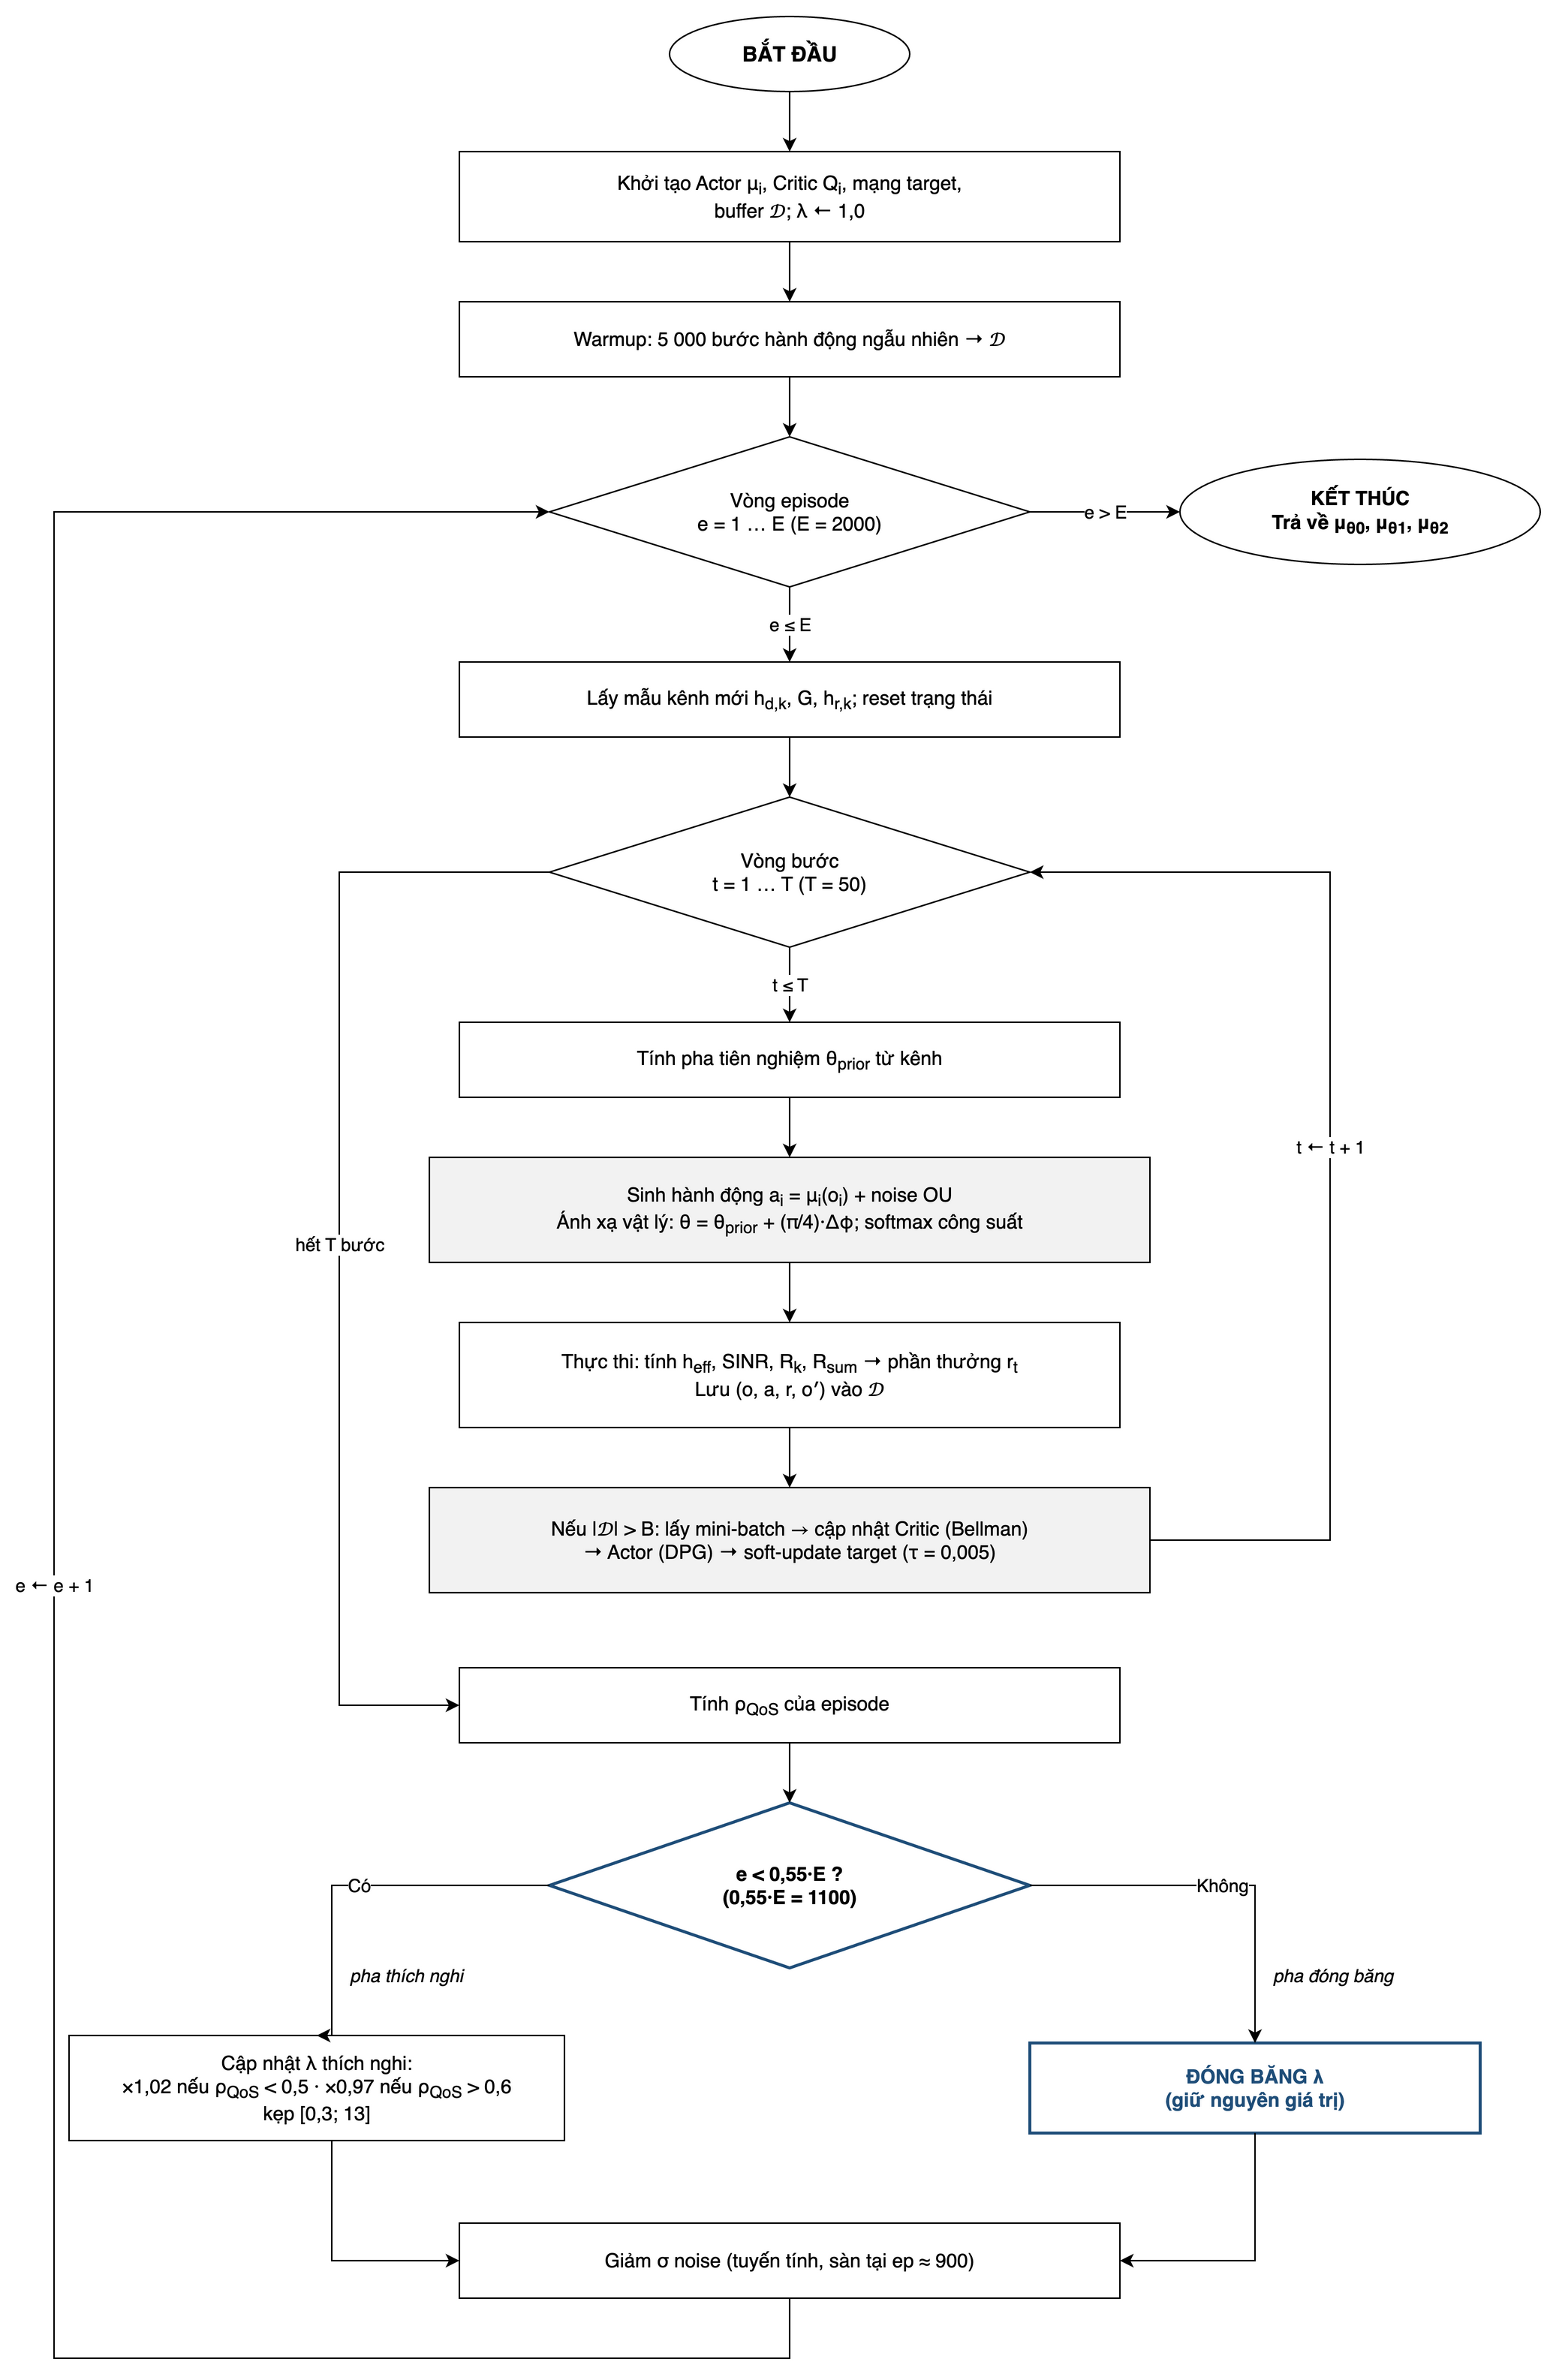
\includegraphics[width=0.78\linewidth]{figures/h3_algorithm_flowchart.png}
  \caption{Sơ đồ luồng thuật toán huấn luyện MADDPG đề xuất, gồm 13
  bước chính từ khởi tạo, warmup, vòng episode lồng vòng step, đến
  cập nhật mạng và hệ số phạt Lagrangian $\lambda$.}
  \label{fig:algo_workflow}
\end{figure}

Sơ đồ phân tách rõ hai vòng lặp lồng nhau: vòng ngoài duyệt qua $E$
episode (mỗi episode: hình học người dùng mới và trạng thái kênh khởi
tạo mới), vòng trong duyệt $T$ khối coherence; trong mỗi khối, tác tử
quan sát kênh hiện hành, ra một quyết định, nhận phần thưởng trên kênh
đó, rồi kênh tiến hóa Gauss--Markov sang khối kế tiếp
\eqref{eq:gauss_markov}. Các khối tô màu đậm (các bước 8 và 12) đánh
dấu các bước có liên quan đến mạng nơ-ron: sinh hành động và cập nhật
Actor-Critic. Các khối còn lại tương ứng với các phép tính kênh truyền,
phần thưởng và quản lý bộ đệm phát lại. Cập nhật các biến đối ngẫu
$\lambda_k$ (bước 13) diễn ra ở cuối mỗi episode theo
\eqref{eq:lambda_update}.

\subsection{Thuật toán huấn luyện chính thức (Algorithm 1)}

\begin{algorithm}[H]
\caption{Proposed MADDPG-Based STAR-RIS RSMA Optimization}
\label{alg:maddpg_train}
\begin{algorithmic}[1]
\Require Số episode $E$, độ dài episode $T$, batch size $B$, kích thước
buffer $|\mathcal{D}|_{\max}$, learning rate $\eta_a, \eta_c$, hệ số
chiết khấu $\gamma$, hệ số cập nhật mềm $\tau$, hệ số phạt khởi tạo
$\lambda_0$, OU noise $\sigma_0 \to \sigma_f$, số bước warmup $T_w$
\Ensure Các Actor đã huấn luyện $\mu_{\theta_0}, \mu_{\theta_1}, \mu_{\theta_2}$
\Statex \textit{// Khởi tạo}
\State Khởi tạo trọng số $\theta_i$ cho Actor $\mu_i$ và $\phi_i$ cho Critic $Q_i$, $i \in \{0, 1, 2\}$
\State Khởi tạo mạng mục tiêu: $\theta_i' \leftarrow \theta_i$, $\phi_i' \leftarrow \phi_i$
\State Khởi tạo replay buffer $\mathcal{D} \leftarrow \emptyset$, $\lambda \leftarrow \lambda_0$
\Statex \textit{// Giai đoạn warmup}
\State Thu thập $T_w = 5{,}000$ chuyển tiếp với hành động ngẫu nhiên đồng đều, lưu vào $\mathcal{D}$
\Statex \textit{// Vòng lặp huấn luyện chính}
\For{$\text{episode} = 1, 2, \ldots, E$}
  \State Lấy mẫu hình học người dùng mới; khởi tạo kênh $h_{d,k}, \mathbf{G}, \mathbf{h}_{r,k}^X \sim \mathcal{CN}(\cdot)$
  \State Khởi tạo trạng thái: $o_{i,1}$ cho $i \in \{0, 1, 2\}$
  \For{$t = 1, 2, \ldots, T$}\Comment{mỗi $t$ là một khối coherence}
    \State Tính tiên nghiệm pha $\theta_n^{\text{prior},X}$ theo công thức \eqref{eq:phase_prior}
    \State $a_{i,t} \leftarrow \mu_{\theta_i}(o_{i,t}) + \mathcal{N}_t^{\text{OU}}$, $i \in \{0, 1, 2\}$
    \State Map $a_{i,t}$ thành tham số vật lý: $\{P_c, P_k, c_k\}$, $\{\theta_n^X, \beta_n^R\}$
    \State Thực thi $\mathbf{a}_t$ trên kênh hiện hành, tính $h_{\text{eff},k}$, $R_k$, $R_{\text{sum}}$
    \State Tính phần thưởng $r_t$ theo \eqref{eq:reward_full} (gồm chi phí tái cấu hình so với $\mathbf{a}_{t-1}$)
    \State Tiến hóa kênh sang khối kế tiếp theo \eqref{eq:gauss_markov}
    \State Lưu chuyển tiếp $(\mathbf{o}_t, \mathbf{a}_t, r_t, \mathbf{o}_{t+1})$ (quan sát THÔ) vào $\mathcal{D}$
    \If{$|\mathcal{D}| > B$}
      \State Lấy mini-batch $\mathcal{B} = \{(\mathbf{o}, \mathbf{a}, r, \mathbf{o}')\}_{j=1}^B$ từ $\mathcal{D}$
      \For{$i \in \{0, 1, 2\}$}
        \State Tính mục tiêu Bellman: $y_i \leftarrow r + \gamma\, Q_{\phi_i'}\!\big(\mathbf{o}', \mu_{\theta_0'}(o_0'), \ldots\big)$
        \State Cập nhật Critic: $\phi_i \leftarrow \phi_i - \eta_c \nabla_{\phi_i} \mathcal{L}_i$ theo \eqref{eq:critic_loss}
        \State Cập nhật Actor: $\theta_i \leftarrow \theta_i + \eta_a \nabla_{\theta_i} J$ theo \eqref{eq:actor_gradient}
        \State Cập nhật mạng mục tiêu: $\theta_i' \leftarrow \tau \theta_i + (1-\tau)\theta_i'$; $\phi_i'$ tương tự
      \EndFor
    \EndIf
  \EndFor
  \State Tính trung bình episode của khe hở ràng buộc: $\bar{c}_k = \frac{1}{T}\sum_t (R_{\min} - R_{k,t})$
  \State Cập nhật $\lambda_k$ theo lịch hai pha \eqref{eq:lambda_freeze}: projected dual gradient \eqref{eq:lambda_update} nếu $\text{episode} < \rho_f E$, ngược lại đóng băng
  \State Giảm OU noise: $\sigma_t$ theo lịch tuyến tính từ $\sigma_0$ về $\sigma_f$
\EndFor
\State \Return $\mu_{\theta_0}, \mu_{\theta_1}, \mu_{\theta_2}$
\end{algorithmic}
\end{algorithm}

% -----------------------------------------------------------------------------
\section{Bảng siêu tham số tổng kết}
\label{sec:hyperparameters}

Bảng \ref{tab:hyperparameters} liệt kê toàn bộ siêu tham số sử dụng để
huấn luyện MADDPG, được chia thành các nhóm: tham số học (learning rate,
hệ số chiết khấu, kích thước batch), tham số khám phá (nhiễu OU, số bước
decay), tham số mạng nơ-ron (kích thước lớp ẩn, activation, gradient
clip) và tham số phần thưởng Lagrangian thích nghi. Các giá trị này
được lựa chọn dựa trên kinh nghiệm thực nghiệm và các khuyến nghị trong
tài liệu chuẩn về DDPG/MADDPG.

\begin{table}[t]
\centering
\caption{Siêu tham số huấn luyện MADDPG-CTDE đề xuất.}
\label{tab:hyperparameters}
\begin{tabular}{p{5.5cm} l}
\toprule
\textbf{Siêu tham số} & \textbf{Giá trị} \\
\midrule
Số episode huấn luyện               & $E = 2\,000$ \\
Độ dài mỗi episode                  & $T = 50$ khối coherence \\
Hệ số tương quan kênh Gauss--Markov & $\rho = 0{,}95$ \\
Số hạt giống huấn luyện             & $8$ \\
Số bước warmup ngẫu nhiên           & $5\,000$ \\
Mốc đóng băng normalizer quan sát   & $5\,000$ bước môi trường \\
Tổng số chuyển tiếp huấn luyện      & $100\,000$ / hạt giống \\
Kích thước replay buffer            & $|\mathcal{D}| = 300\,000$ (quan sát thô) \\
Batch size                          & $B = 256$ \\
Hệ số chiết khấu                    & $\gamma = 0{,}95$ \\
Hệ số cập nhật mềm                  & $\tau = 0{,}005$ \\
Learning rate Actor                 & $\eta_a = 10^{-4}$ \\
Learning rate Critic                & $\eta_c = 5 \times 10^{-4}$ \\
Số lớp ẩn                           & $2$ (mỗi lớp $256$ đơn vị) \\
Activation                          & ReLU + LayerNorm \\
Output activation Actor             & tanh \\
Gradient clip (norm)                & $1{,}0$ \\
Nhiễu OU $\sigma_0 \to \sigma_f$    & $0{,}4 \to 0{,}05$ \\
Số bước decay nhiễu                 & $45\,000$ (episode $\approx 900$) \\
Ánh xạ pha cấu hình chính          & Pha tuyệt đối, $	heta_n=\pi(a_n+1)$ \\
$\lambda_k$ ban đầu                 & $1{,}0$ (mỗi người dùng) \\
Miền chiếu $\lambda_k$              & $[0,\, 20]$ \\
Tốc độ học đối ngẫu $\eta_{\lambda}$ & $0{,}01$ (EMA $0{,}9$) \\
Tỷ lệ đóng băng $\lambda$ ($\rho_f$) & $0{,}55$ (episode $1\,100$) \\
Hệ số $\alpha$ sum-rate / $R_{\text{ref}}$ & $1{,}5$ / $20$ b/s/Hz \\
Trọng số augmented penalty $w$      & $1{,}0$ \\
Trọng số switching cost $\eta_{\phi}/\eta_{P}/\eta_{\beta}$ & $0{,}1 / 0{,}05 / 0{,}05$ \\
Reward clip                         & $[-50,\, +50]$ \\
\bottomrule
\end{tabular}
\end{table}

% -----------------------------------------------------------------------------
\section{Phân tích độ phức tạp tính toán}
\label{sec:complexity}

\subsection{Độ phức tạp huấn luyện}

Mỗi bước cập nhật yêu cầu một lần chạy tiến/ngược qua các Actor và Critic.
Với 3 tác tử và Critic kích thước $821 \to 256 \to 256 \to 1$:
\begin{equation}
\mathcal{C}_{\text{train,step}} = O\!\big(3 \times (256^2 + 256 \times 821)\big)
                                = O(10^5)\ \text{ops}.
\end{equation}
Tổng cộng $100\,000$ bước cập nhật mỗi hạt giống cho thấy chi phí huấn
luyện vào khoảng $10^{10}$ phép toán nổi, tương đương vài giờ trên CPU
thông thường hoặc dưới một giờ trên GPU phổ thông (đo thực tế ở pipeline
cũ: $\approx 40$ phút/hạt giống trên GPU T4).

\subsection{Độ phức tạp suy luận}

Tại thời điểm thực thi, chỉ Actor được dùng:
\begin{equation}
\mathcal{C}_{\text{infer}} = O\!\big(|o_i| \times 256 + 256^2 + 256 \times |a_i|\big)
                            \approx O(10^4)\ \text{ops/agent}.
\end{equation}
Mỗi khối coherence chỉ cần đúng một lần suy luận (một quyết định cho
một khối), nên độ trễ suy luận cỡ mili-giây là phù hợp với nhịp cập
nhật theo khối pha-đinh (vài ms tới hàng chục ms). Độ trễ được đo bằng
hai benchmark riêng biệt --- CPU (một luồng, ép toàn bộ mô hình về CPU)
và GPU (đồng bộ hóa CUDA quanh vùng đo) --- trình bày ở Chương 4; hai
bảng không được so sánh trực tiếp với nhau. Số đo tham chiếu của
pipeline cũ ($\approx 1{,}3$ ms/hành động) được thực hiện với
device=auto (GPU T4) nên chỉ có giá trị định hướng; kết luận chính
thức dùng cặp bảng CPU/GPU mới.

% -----------------------------------------------------------------------------
\section*{Kết luận chương}
\addcontentsline{toc}{section}{Kết luận chương}

Chương 3 đã trình bày chi tiết khuôn khổ MADDPG-CTDE ba tác tử chuyên
dụng để giải bài toán surrogate của P0. Ba cải tiến quan trọng được đề
xuất: (i) ánh xạ pha tuyệt đối nhất quán với cấu hình đã khóa
$4^N$ lần và cung cấp một điểm khởi đầu hợp lý; (ii) hàm phần thưởng
Lagrangian surrogate với các biến đối ngẫu $\lambda_k$ per-user cập
nhật bằng projected dual gradient trên khe hở ràng buộc có dấu, tự điều
chỉnh cân bằng giữa tổng tốc độ và mức đáp ứng QoS; (iii) lịch trình
heuristic hai pha đóng băng $\boldsymbol{\lambda}$ (two-stage dual
freeze) làm cho hàm phần thưởng trở nên dừng ở $45\%$ cuối huấn luyện,
giúp đường cong huấn luyện dễ diễn giải (không phải một bảo đảm hội
tụ). Cùng với các
kỹ thuật chuẩn (replay buffer, target networks, OU noise, warmup,
gradient clip), khuôn khổ đề xuất hội tụ ổn định và đạt hiệu năng
cạnh tranh, điều sẽ được kiểm chứng thực nghiệm ở Chương 4 --- bao gồm
cả thí nghiệm khả năng mở rộng theo số phần tử $N$ nhằm định lượng
lợi thế của kiến trúc phân rã đa tác tử.


% Chương 4
% =============================================================================
%  CHƯƠNG 4 – KẾT QUẢ MÔ PHỎNG VÀ ĐÁNH GIÁ
% =============================================================================
\chapter{KẾT QUẢ MÔ PHỎNG VÀ ĐÁNH GIÁ}
\label{ch:chuong4}

Chương này trình bày kết quả mô phỏng số học để đánh giá hiệu năng của
khuôn khổ MADDPG-CTDE đề xuất so với các thuật toán DRL tham chiếu và các
phương pháp xử lý STAR-RIS truyền thống. Các kết quả được phân thành các
nhóm: (1) thiết lập mô phỏng (mục \ref{sec:setup}), (2) hội tụ huấn
luyện (mục \ref{sec:convergence}), (3) so sánh thuật toán DRL (mục
\ref{sec:algo_comp}), (4) độ nhạy với công suất phát (mục \ref{sec:power_sweep}),
(5) khả năng mở rộng theo số phần tử STAR-RIS (mục \ref{sec:scalability}),
(6) phân tích loại trừ cho STAR-RIS (mục \ref{sec:ablation}) và (7) phân
tích chuyên sâu (mục \ref{sec:deep_analysis}).

\noindent\fbox{\parbox{0.97\linewidth}{\small\textbf{Ghi chú về nguồn số
liệu (bản nháp --- PENDING).} Các con số trong chương này được sinh bởi
pipeline mô phỏng phiên bản trước refactor 2026-07-16 (formulation
block-fading tĩnh trong episode, chỉ số QoS đo ``tất cả người dùng đồng
thời đạt ngưỡng'', baseline AO-Grid khi đó bị gọi là BCD, vùng tin cậy
của hình hội tụ tính bằng rolling std). Toàn bộ bảng và hình của chương
sẽ được tái sinh bằng pipeline Dynamic-MDP mới (mô tả ở Chương 2--3)
theo quy trình trong \texttt{KAGGLE\_RERUN\_CHECKLIST.md}; kết quả cũ
được lưu tại \texttt{results\_legacy/} và không dùng làm bằng chứng
cuối cùng. Các định nghĩa metric và cách tính thống kê nêu dưới đây là
của pipeline mới.}}

% -----------------------------------------------------------------------------
\section{Thiết lập mô phỏng}
\label{sec:setup}

\subsection{Tham số hệ thống và phần cứng}

Hệ thống STAR-RIS RSMA được mô phỏng bằng Python 3.10 với PyTorch 2.x.
Bảng \ref{tab:simulation_parameters} liệt kê toàn bộ tham số mô phỏng,
được trích xuất tự động từ tệp cấu hình \texttt{config.yaml} của thư
viện mã nguồn để đảm bảo tính tái lập.

\begin{table}[t]
\centering
\small
\caption{Tham số mô phỏng đầy đủ của hệ thống và thuật toán.}
\label{tab:simulation_parameters}
\begin{tabular}{ll}
\toprule
\textbf{Tham số} & \textbf{Giá trị} \\
\midrule
\multicolumn{2}{l}{\textbf{Cấu hình hệ thống}} \\
Số người dùng tổng ($K$) & 4 \\
Số người dùng vùng phản xạ ($K_R$) & 3 \\
Số phần tử STAR-RIS ($N$) & 32 \\
Số anten BS ($M$) & 4 \\
Công suất phát tối đa $P_{\max}$ & $30$ dBm \\
Công suất tạp âm $\sigma^2$ & $-90$ dBm \\
QoS tối thiểu $R_{\min}$ & $0{,}3$ b/s/Hz \\
Suy hao chướng ngại UE$_T$ & $25$ dB \\
Số mũ suy hao kênh trực tiếp $\alpha_d$ & $3{,}5$ \\
Số mũ suy hao kênh BS-RIS $\alpha_G$ & $2{,}2$ \\
Số mũ suy hao kênh RIS-UE $\alpha_r$ & $2{,}5$ \\
\midrule
Hệ số tương quan kênh Gauss--Markov $\rho$ & $0{,}95$ \\
\midrule
\multicolumn{2}{l}{\textbf{Tham số hàm phần thưởng (Lagrangian surrogate)}} \\
Hệ số $\alpha$ sum-rate / $R_{\text{ref}}$ & $1{,}5$ / $20$ b/s/Hz \\
Trọng số augmented penalty $w$ & $1{,}0$ \\
$\lambda_k$ ban đầu / miền chiếu & $1{,}0$ / $[0,\,20]$ \\
Tốc độ học đối ngẫu $\eta_\lambda$ / EMA & $0{,}01$ / $0{,}9$ \\
Tỷ lệ đóng băng $\lambda$ ($\rho_f$) & $0{,}55$ \\
Trọng số switching cost $\eta_\phi/\eta_P/\eta_\beta$ & $0{,}1$ / $0{,}05$ / $0{,}05$ \\
Ánh xạ pha mặc định & Pha tuyệt đối, $\phi_n=\pi(a_n+1)$ \\
\midrule
\multicolumn{2}{l}{\textbf{Tham số huấn luyện}} \\
Số episode mỗi thuật toán & $2\,000$ \\
Số hạt giống huấn luyện & $8$ (cấu hình chuẩn và sweep $N$) \\
Hạt giống validation / test (khóa) & $[11,\ldots,55]$ / $[70001,\ldots,70005]$ \\
Nguồn seed split / SHA-256 & \texttt{seed\_split.v1.yaml} / \texttt{d73ba5aea6d0\ldots f118854} \\
Số bước warmup ngẫu nhiên & $5\,000$ \\
Mốc đóng băng normalizer quan sát & $5\,000$ bước môi trường \\
Số bước decay nhiễu OU & $45\,000$ \\
\bottomrule
\end{tabular}

\vspace{0.2em}
\hfill {\footnotesize\itshape Nguồn: Tác giả xây dựng (2026)}
\end{table}


\subsection{Các baseline được so sánh}

Để đánh giá khách quan, MADDPG đề xuất được so sánh với tám baseline,
chia làm hai nhóm:

\noindent\textbf{Nhóm A, Các thuật toán DRL đơn tác tử / đa tác tử khác:}
\begin{itemize}[leftmargin=*]
\item \textbf{DDPG} \cite{lillicrap2016continuous}: tác tử đơn với hành
động 140 chiều hợp nhất.
\item \textbf{TD3} \cite{fujimoto2018addressing}: cải tiến của DDPG với
hai Critic và trì hoãn cập nhật Actor.
\item \textbf{PPO} \cite{schulman2017proximal}: thuật toán on-policy với
clip surrogate objective.
\end{itemize}

\noindent\textbf{Nhóm B, Các phương pháp xử lý STAR-RIS truyền thống:}
\begin{itemize}[leftmargin=*]
\item \textbf{AO-Grid}: heuristic tối ưu xen kẽ dạng lưới thô
(coarse alternating-optimization grid): pha lấy nghiệm phân tích căn
đồng pha cho người dùng yếu nhất, một hệ số $\beta$ chung cho mọi phần
tử tìm trên lưới 5 điểm, tỷ lệ $P_c/P_{\max}$ tìm trên lưới 6 điểm,
công suất riêng và tỷ lệ tách chia đều. Đây là một \emph{heuristic tham
chiếu}, không phải cận trên tối ưu và không xử lý ràng buộc QoS.
(Trong pipeline cũ phương pháp này bị gọi nhầm là ``BCD/cận trên''.)
\item \textbf{Hybrid AO Local Search} (SLSQP + projected gradient): tìm
kiếm cục bộ xen kẽ trên đúng không gian biến của P0 (vector
$\beta_n^R$ per-element, pha, công suất, tỷ lệ tách), đa điểm khởi
tạo, cùng hàm mục tiêu surrogate và chi phí tái cấu hình như DRL;
chạy cho $N \leq 32$. Là mốc tham chiếu tìm kiếm cục bộ, không phải
cận trên.
\item \textbf{MaxMinAligned}: căn pha đồng pha cho người dùng yếu nhất,
sử dụng công thức \eqref{eq:phase_prior} mà không có RL tinh chỉnh.
\item \textbf{FixedRIS}: $\beta_n^R = \beta_n^T = 1/2$, $\theta_n^X = 0$ cho
mọi $n$.
\item \textbf{RandomRIS}: pha ngẫu nhiên đều trong $[0, 2\pi)$ cho mọi
phần tử, biên độ ngẫu nhiên trong $[0,1]$.
\item \textbf{NoRIS}: bỏ STAR-RIS, chỉ giữ kênh trực tiếp $h_{d,k}$.
\end{itemize}
Nhóm A còn bổ sung \textbf{TD3-Matched}: TD3 đơn tác tử với bề rộng lớp
ẩn được chọn tự động sao cho \emph{tổng} tham số khả huấn luyện khớp
MADDPG trong sai lệch $5\%$, dùng để tách bạch lợi ích của phân rã đa
tác tử khỏi lợi ích thuần túy về dung lượng mạng.

\subsection{Phương pháp đánh giá}

Tất cả các kết quả tại cấu hình chuẩn $N=32$ được lấy trung bình trên
$8$ hạt giống huấn luyện độc lập $\{1000, 2000, \ldots, 8000\}$; đơn vị
phân tích thống kê là \emph{trung bình theo hạt giống huấn luyện}: mỗi
hạt giống được đánh giá xác định (deterministic) trên cùng một tập kịch
bản kiểm tra đã khóa (ScenarioBank: hình học người dùng, kênh khởi tạo
và chuỗi innovation Gauss--Markov sinh trước, giống hệt nhau cho mọi
phương pháp), rồi khoảng tin cậy $95\%$ Student-t được tính qua $8$ giá
trị trung bình đó. Các baseline không học (AO-Grid, MaxMinAligned,
FixedRIS, \ldots) không phụ thuộc hạt giống huấn luyện nên độ bất định
của chúng được tính qua các kịch bản đánh giá độc lập. Tập hạt giống
$\{11, \ldots, 55\}$ trước đây --- đã được xem trong quá trình phát
triển --- chỉ dùng làm \emph{validation} (chọn mô hình, tinh chỉnh);
kết quả báo cáo dùng tập kịch bản kiểm tra khóa sinh từ các hạt giống
mới $\{81011, 81023, 81041, 81071, 81101\}$. Danh sách phát triển, validation,
legacy $\{9101,\ldots,9505\}$ và final-test được đăng ký duy nhất tại
\texttt{config/seed\_split.v2.yaml}, SHA-256
\texttt{dc327042efcad7007efa0006f0b10461eb69055992a3cdcd6416612d15db13e8};
pipeline từ chối chạy nếu hash không khớp. Riêng thí nghiệm khả năng mở rộng theo
$N$ (mục \ref{sec:scalability}) sử dụng $10$ hạt giống huấn luyện cho
mỗi điểm cấu hình. Kiểm định ý nghĩa thống kê dùng thiết kế theo cặp
(cùng danh sách hạt giống huấn luyện, cùng kịch bản đánh giá): paired
t-test và sign-flip permutation test trên các trung bình mức hạt
giống, hiệu chỉnh Holm--Bonferroni cho họ bốn so sánh chính
$\{$MADDPG vs TD3, TD3-Matched, DDPG, PPO$\}$ trên sum-rate; kích thước hiệu ứng
(Cohen's d theo cặp) và CI của hiệu số được báo cáo kèm (Bảng
\ref{tab:significance}).

% -----------------------------------------------------------------------------
\section{Hội tụ huấn luyện}
\label{sec:convergence}

\subsection{Đường cong hội tụ về tổng phần thưởng}

Hình \ref{fig:training_convergence} thể hiện đường cong hội tụ của tổng
phần thưởng (Return) theo episode đối với các thuật toán DRL trên
$2\,000$ episode. Mỗi đường của từng hạt giống được làm trơn riêng
(trung bình trượt), sau đó tại từng episode tính trung bình và khoảng
tin cậy $95\%$ Student-t \emph{qua $8$ hạt giống huấn luyện}; vùng tô
bóng là khoảng tin cậy giữa các hạt giống này.

\begin{figure}[t]
  \centering
  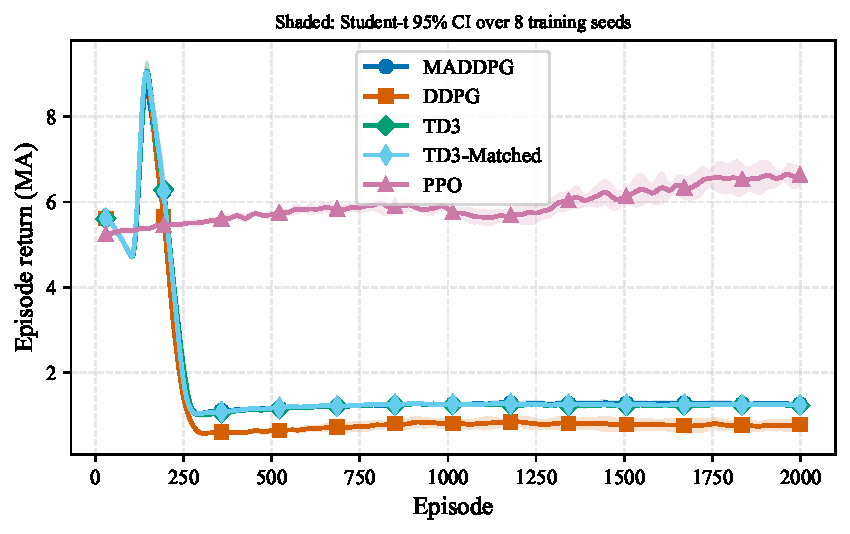
\includegraphics[width=0.85\linewidth]{figures/training_convergence.pdf}
  \caption{Đường cong hội tụ tổng phần thưởng (Return) theo episode trên
  8 hạt giống huấn luyện độc lập. Vùng bóng mờ là khoảng tin cậy $95\%$
  Student-t giữa các hạt giống (mỗi hạt giống được làm trơn riêng trước
  khi tổng hợp).}
  \label{fig:training_convergence}
\end{figure}

Có thể thấy: PPO hội tụ chậm và đều nhờ cập nhật on-policy bảo thủ.
MADDPG khởi đầu chậm do cần làm đầy replay buffer, sau đó tăng nhanh
và đạt vùng bão hòa quanh episode $700$--$1\,000$. Kể từ mốc đóng băng
$\boldsymbol{\lambda}$ (episode $1\,100$), hàm phần thưởng trở nên dừng
và các đường cong đi ngang ổn định. Lưu ý về diễn giải: vùng phẳng này
cho thấy phần thưởng đã dừng và chính sách ổn định theo thang đo đó;
nó \emph{không} tự nó chứng minh chính sách đã hội tụ về nghiệm tối
ưu.

\subsection{Tổng tốc độ qua các episode}

Hình \ref{fig:training_sum_rate} cho thấy tổng tốc độ $R_{\text{sum}}$
trung bình theo episode. Đây là chỉ số trực tiếp phản ánh mục tiêu của
bài toán P0.

\begin{figure}[t]
  \centering
  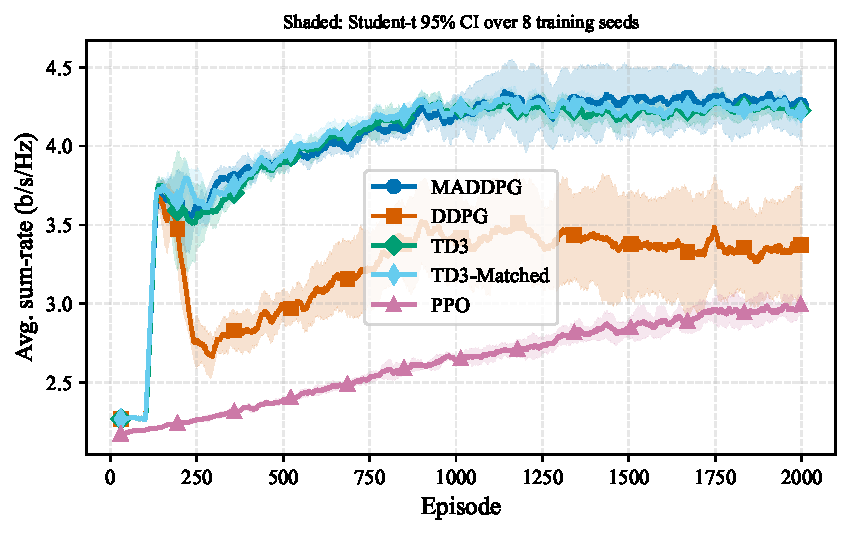
\includegraphics[width=0.85\linewidth]{figures/training_sum_rate.pdf}
  \caption{Tổng tốc độ $R_{\text{sum}}$ (b/s/Hz) theo episode trong quá
  trình huấn luyện (trung bình 8 hạt giống). MADDPG và TD3 hội tụ về
  sum-rate cao nhất và đạt trạng thái phẳng ở nửa cuối.}
  \label{fig:training_sum_rate}
\end{figure}

Ba thuật toán đạt sum-rate cao nhất sau khi hội tụ là MADDPG ($\sim 4{,}52$
b/s/Hz), TD3-Matched ($\sim 4{,}41$) và TD3 ($\sim 4{,}39$) --- gần như trùng
nhau. PPO có sum-rate thấp hơn ($\sim 3{,}42$) vì
PPO ưu tiên thỏa mãn QoS tuyệt đối (xem hình tiếp theo). DDPG đơn tác tử có
sum-rate thấp nhất ($\sim 3{,}94$); so sánh chi tiết với TD3 --- đơn tác tử mạnh
nhất --- được trình bày ở mục \ref{sec:algo_comp} và \ref{sec:scalability}.

\subsection{Xác suất thỏa mãn QoS}

Luận văn phân biệt rõ hai chỉ số QoS
(\eqref{eq:user_qos_fraction}--\eqref{eq:all_users_qos}): tỷ lệ người
dùng đạt ngưỡng (user QoS fraction) và xác suất \emph{tất cả} $K$ người
dùng đồng thời đạt ngưỡng (all-users QoS). Hình
\ref{fig:training_qos_prob} biểu diễn chỉ số theo episode trong quá
trình huấn luyện; pipeline mới vẽ cả hai chỉ số trên hai hình riêng và
mỗi hình ghi rõ metric.

\begin{figure}[t]
  \centering
  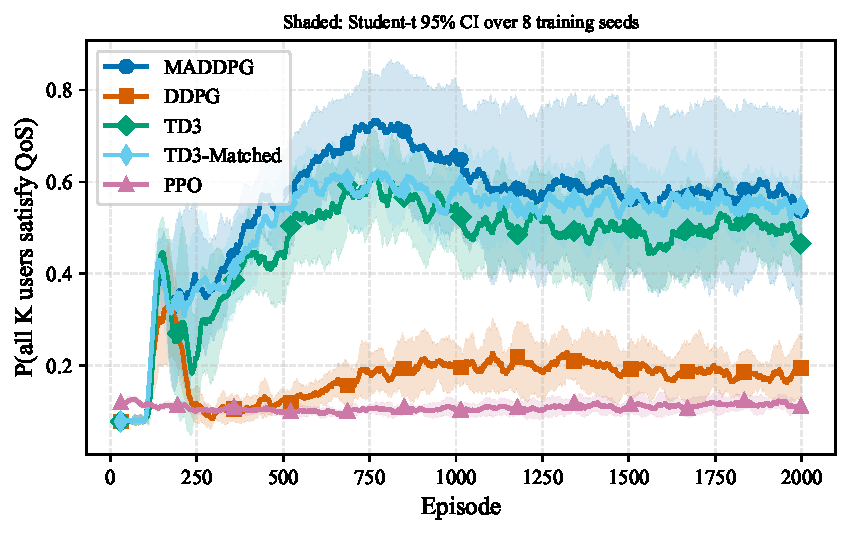
\includegraphics[width=0.85\linewidth]{figures/training_qos_prob.pdf}
  \caption{Chỉ số thỏa mãn QoS theo episode: xác suất tất cả $K=4$
  người dùng đồng thời đạt $R_{\min}$ (all-users QoS). MADDPG đạt mức
  cao nhất ($\approx 0{,}61$) tại cấu hình chuẩn $N=32$.}
  \label{fig:training_qos_prob}
\end{figure}

MADDPG đạt all-users QoS $\approx 0{,}61$ --- cao nhất trong các thuật
toán DRL tại $N=32$ --- trong khi vẫn giữ sum-rate cao nhất; cần nhấn
mạnh rằng con số này là \emph{xác suất cả bốn người dùng đồng thời đạt
$R_{\min}$} (all-users QoS), không phải tỷ lệ người dùng đạt ngưỡng ---
tỷ lệ người dùng đạt ngưỡng (QoS/UE) luôn cao hơn, với MADDPG đạt
$\approx 0{,}84$. Điểm vận hành có thể dịch chuyển thêm về phía QoS
bằng cách tăng miền chiếu $\lambda_{\max}$. Điều đó phản ánh đúng bản chất surrogate của hàm
phần thưởng: các biến đối ngẫu $\lambda_k$ điều chỉnh cân bằng giữa hai
mục tiêu, và điểm vận hành có thể dịch chuyển về phía QoS bằng cách
tăng miền chiếu $\lambda_{\max}$ (mục \ref{sec:tradeoff_discussion}).

\subsection{Sự tiến hóa của các biến đối ngẫu $\lambda_k$}

Hình \ref{fig:qos_lambda} cho thấy động học của các biến đối ngẫu theo
thời gian huấn luyện (pipeline mới ghi log từng $\lambda_k$ riêng).
Biểu đồ này giúp kiểm chứng hoạt động của cập nhật projected dual
gradient và lịch trình hai pha (two-stage dual freeze).

\begin{figure}[t]
  \centering
  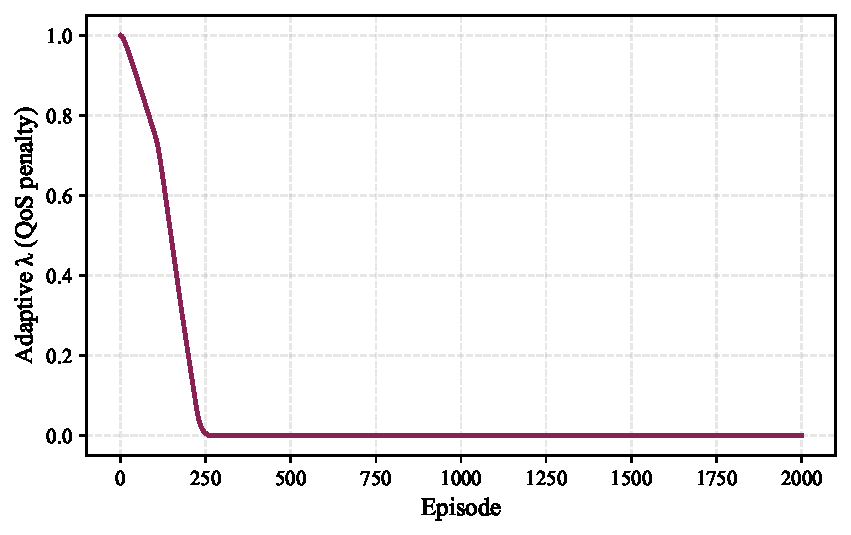
\includegraphics[width=0.85\linewidth]{figures/qos_lambda.pdf}
  \caption{Sự tiến hóa của các biến đối ngẫu $\lambda_k$ theo lịch
  trình hai pha: pha cập nhật đối ngẫu và pha đóng băng từ episode
  $1\,100$ ($55\%$ của $2\,000$ episode, phần thưởng dừng). Hình hiển
  thị vector $\lambda_k$ per-user của pipeline Dynamic-MDP.}
  \label{fig:qos_lambda}
\end{figure}

Trong pha cập nhật, $\lambda_k$ tăng khi người dùng $k$ vi phạm ràng
buộc theo kỳ vọng và giảm khi có slack (khe hở có dấu), đúng hành vi
hai chiều của gradient đối ngẫu; việc một số $\lambda_k$ bám sát biên
trên cho thấy ràng buộc QoS bó chặt với hình học kênh khảo sát.
Kể từ mốc đóng băng (episode $1\,100$), $\boldsymbol{\lambda}$ được giữ
nguyên theo \eqref{eq:lambda_freeze}: hàm phần thưởng trở nên dừng và
đường Return ở Hình \ref{fig:training_convergence} nhờ đó có thể đi
ngang.

Về cấu trúc phần thưởng: phép ánh xạ softmax của tác tử BS bảo đảm
$P_c + \sum_k P_k = P_{\max}$ theo cấu trúc nên ràng buộc (C1) tự động
được thỏa; vì lý do đó pipeline mới đã loại hẳn số hạng phạt công suất
(một số hạng luôn bằng không) khỏi hàm phần thưởng. Phần thưởng được
chi phối bởi cân bằng giữa thành phần sum-rate, thành phần đối ngẫu
QoS và chi phí tái cấu hình --- đúng như thiết kế ở Chương 3.

% -----------------------------------------------------------------------------
\section{So sánh các thuật toán DRL}
\label{sec:algo_comp}

\subsection{Bảng so sánh tổng hợp}

Bảng \ref{tab:algorithm_comparison} so sánh hiệu năng của MADDPG với
các thuật toán DRL đơn tác tử trên các chỉ số: Return, Sum-rate, xác
suất QoS, tốc độ luồng chung $R_c$, entropy pha, tỷ lệ $P_c/P_{\max}$,
độ trễ suy luận, và $\lambda$ huấn luyện cuối cùng.

\begin{table}[t]
\centering
\small
\caption{So sánh hiệu năng các thuật toán DRL trên locked test ScenarioBank tại cấu hình chuẩn $N=32$ (pipeline Dynamic-MDP; đơn vị phân tích = trung bình theo hạt giống huấn luyện, khoảng tin cậy Student-t $95\%$ qua $8$ hạt giống). Return theo tập bị lược khỏi so sánh chéo vì vector $\lambda$ tối ưu khác nhau giữa các thuật toán; các cột dưới là chỉ số vật lý. QoS all-users là $\Pr[\min_k R_k \ge R_{\min}]$; QoS/UE là $(1/K)\sum_k \mathbf{1}[R_k \ge R_{\min}]$.}
\label{tab:algorithm_comparison}
\setlength{\tabcolsep}{4pt}
\begin{tabular}{lcccccc}
\toprule
\textbf{Thuật toán} & \textbf{Sum-rate} & \textbf{QoS} & \textbf{QoS/UE} & \textbf{$R_c$} & \textbf{$P_c/P_{\max}$} & \textbf{Trễ CPU} \\
                    & (b/s/Hz)          & (all-users)   &                &                &                         & (ms)               \\
\midrule
\textbf{MADDPG} & $\mathbf{4{,}52 \pm 0{,}20}$ & $\mathbf{0{,}61}$ & $0{,}84$ & $2{,}24$ & $0{,}79$ & $0{,}60$ \\
TD3-Matched     & $4{,}41 \pm 0{,}06$         & $0{,}55$          & $0{,}84$ & $\mathbf{2{,}45}$ & $\mathbf{0{,}84}$ & $0{,}27$ \\
TD3             & $4{,}39 \pm 0{,}06$         & $0{,}45$          & $0{,}80$ & $2{,}24$ & $0{,}81$ & $\mathbf{0{,}25}$ \\
DDPG            & $3{,}94 \pm 0{,}36$         & $0{,}40$          & $0{,}75$ & $1{,}76$ & $0{,}68$ & $0{,}25$ \\
PPO             & $3{,}42 \pm 0{,}18$         & $0{,}39$          & $0{,}77$ & $1{,}49$ & $0{,}59$ & $0{,}49$ \\
\bottomrule
\end{tabular}

\vspace{0.2em}
{\footnotesize Ghi chú: Giá trị in đậm là tốt nhất theo từng cột. MADDPG đạt sum-rate và QoS all-users thô cao nhất, nhưng kiểm định paired ($n=8$) $+$ Holm (Bảng \ref{tab:significance}) cho thấy \emph{không} khác biệt có ý nghĩa so với TD3, TD3-Matched hay DDPG; chỉ vượt PPO có ý nghĩa. $R_c$: tốc độ luồng chung; $P_c/P_{\max}$: tỷ lệ công suất luồng chung. Cột trễ đo trên CPU một luồng, $2000$ lần gọi (Bảng \ref{tab:latency_cpu}); heuristic AO-Grid tốn $13{,}97$ ms/quyết định trên cùng phần cứng.\par}
\hfill {\footnotesize\itshape Nguồn: Tác giả xây dựng (2026)}
\end{table}


\textbf{Quan sát chính:}
\begin{itemize}[leftmargin=*]
\item \textbf{Sum-rate:} MADDPG đạt $4{,}52 \pm 0{,}20$ b/s/Hz, cao hơn
DDPG ($3{,}94 \pm 0{,}36$) tới $+15\%$ và nhỉnh hơn TD3
($4{,}39 \pm 0{,}06$) lẫn TD3-Matched ($4{,}41 \pm 0{,}06$). Tại cấu
hình chuẩn $N=32$, MADDPG, TD3 và TD3-Matched là ba phương pháp dẫn
đầu và tương đương nhau về mặt thống kê (Bảng \ref{tab:significance});
sự tương đương này kéo dài theo quy mô $N$ (mục \ref{sec:scalability}).
\item \textbf{Tỷ lệ $P_c/P_{\max} \approx 0{,}79$} ở MADDPG cho thấy
phần lớn năng lượng được dành cho luồng chung, phù hợp với cấu trúc
RSMA khi có UE rất yếu ở vùng truyền qua; tốc độ luồng chung
$R_c = 2{,}24$ b/s/Hz chiếm gần một nửa tổng tốc độ.
\item \textbf{Độ trễ suy luận} MADDPG đo được $\approx 0{,}60$ ms/hành
động trên CPU một luồng (Bảng \ref{tab:latency_cpu}), thấp hơn một bậc
so với heuristic AO-Grid ($13{,}97$ ms) giải lại cho từng channel
realization (mục \ref{sec:complexity_analysis}).
\end{itemize}

\subsection{Kiểm định ý nghĩa thống kê và thảo luận về số hạt giống}

Bảng \ref{tab:significance} liệt kê kết quả kiểm định theo cặp giữa
MADDPG và mỗi baseline: vì mọi thuật toán được huấn luyện trên cùng
danh sách hạt giống và đánh giá trên cùng tập kịch bản khóa, thiết kế
theo cặp (paired t-test và sign-flip permutation test trên các trung
bình mức hạt giống) có sức mạnh thống kê cao hơn Welch không bắt cặp
mà pipeline cũ sử dụng. Họ so sánh chính gồm ba giả thuyết
$\{$MADDPG vs TD3, DDPG, PPO$\}$ trên sum-rate và được hiệu chỉnh
Holm--Bonferroni ($m=3$); các chỉ số phụ (QoS, Return) được báo cáo
trong họ riêng với hiệu chỉnh riêng. Việc kiểm định trên sum-rate và
QoS (thay vì chỉ Return) là cần thiết vì Return chịu ảnh hưởng của bộ
$\lambda_k$ khác nhau giữa các thuật toán, trong khi sum-rate và QoS
là các đại lượng vật lý so sánh được trực tiếp.

\begin{table}[t]
\centering
\small
\caption{Kiểm định thống kê theo cặp giữa MADDPG và các baseline trên sum-rate (locked test bank, $N=32$; trung bình mức hạt giống, $n=8$ cặp). Pipeline Dynamic-MDP dùng paired t-test $+$ sign-flip permutation với hiệu chỉnh Holm--Bonferroni cho họ bốn so sánh chính $\{$MADDPG vs TD3, TD3-Matched, DDPG, PPO$\}$. Cohen's $d$ theo cặp đo kích thước hiệu ứng.}
\label{tab:significance}
\begin{tabular}{lcccc}
\toprule
\textbf{So sánh (sum-rate)} & \textbf{$\Delta$ trung bình} & \textbf{Cohen's $d$} & \textbf{$p_{\text{Holm}}$} & \textbf{Có ý nghĩa (5\%)} \\
\midrule
MADDPG vs TD3         & $+0{,}13 \pm 0{,}24$ & $0{,}45$ & $0{,}45$ & Không \\
MADDPG vs TD3-Matched & $+0{,}11 \pm 0{,}19$ & $0{,}47$ & $0{,}45$ & Không \\
MADDPG vs DDPG        & $+0{,}58 \pm 0{,}49$ & $0{,}98$ & $0{,}081$ & Không \\
MADDPG vs PPO         & $+1{,}10 \pm 0{,}16$ & $5{,}64$ & $\mathbf{3{,}7 \times 10^{-6}}$ & \textbf{Có} \\
\bottomrule
\end{tabular}

\vspace{0.2em}
{\footnotesize Ghi chú: Sau hiệu chỉnh Holm, MADDPG chỉ vượt PPO có ý nghĩa thống kê; so với TD3, TD3-Matched và DDPG thì \emph{không} khác biệt có ý nghĩa ở mức $5\%$. Đáng chú ý, MADDPG không vượt được TD3-Matched (biến thể tác tử đơn có \emph{cùng tổng số tham số}, xem Bảng \ref{tab:complexity}), cho thấy kiến trúc phân rã đa tác tử không mang lại lợi thế thống kê ở cấu hình này. Với DDPG, hiệu số lớn ($d=0{,}98$) nhưng chưa đạt ngưỡng sau hiệu chỉnh do cỡ mẫu $n=8$ hạn chế lực kiểm định. Kết luận này nhất quán với thí nghiệm mở rộng theo $N$ (Bảng \ref{tab:scalability}): MADDPG tương đương TD3 ở mọi $N$.\par}
\hfill {\footnotesize\itshape Nguồn: Tác giả xây dựng (2026)}
\end{table}


\textbf{Diễn giải khách quan kết quả thống kê:}
\begin{itemize}[leftmargin=*]
\item \textbf{Sum-rate so với PPO ($p_{\text{Holm}} = 3{,}7 \times 10^{-6}$):}
MADDPG vượt PPO với ý nghĩa thống kê rất mạnh --- chênh lệch $+1{,}10$
b/s/Hz, kích thước hiệu ứng rất lớn ($d = 5{,}6$). Đây là baseline duy
nhất mà MADDPG vượt qua có ý nghĩa sau hiệu chỉnh Holm.
\item \textbf{Sum-rate so với DDPG ($p_{\text{Holm}} = 0{,}081$):} chênh
lệch $+0{,}58$ b/s/Hz với kích thước hiệu ứng lớn ($d = 0{,}98$) nhưng
\emph{chưa} đạt ngưỡng ý nghĩa sau hiệu chỉnh Holm do cỡ mẫu $n=8$ hạn
chế lực kiểm định; không thể kết luận vượt trội có ý nghĩa.
\item \textbf{Sum-rate so với TD3 ($p_{\text{Holm}} = 0{,}45$) và
TD3-Matched ($p_{\text{Holm}} = 0{,}45$):} tại $N=32$, chênh lệch chỉ
$+0{,}13$ và $+0{,}11$ b/s/Hz, không có ý nghĩa thống kê; MADDPG tương
đương cả hai tác tử đơn mạnh nhất --- kể cả biến thể TD3-Matched có
cùng tổng số tham số. Thí nghiệm mở rộng theo $N$ (mục
\ref{sec:scalability}) xác nhận sự tương đương này kéo dài tới $N=128$.
\item \textbf{Về Return:} PPO có Return cao hơn nhưng điều này không
đồng nghĩa hiệu năng vật lý tốt hơn --- Return chịu ảnh hưởng của bộ
$\lambda_k$ khác nhau giữa các thuật toán nên bị lược khỏi so sánh chéo;
xét sum-rate thực tế, PPO thấp hơn MADDPG $1{,}10$ b/s/Hz.
\end{itemize}

\textbf{Lưu ý về quy mô thí nghiệm.} Số hạt giống huấn luyện được
nâng từ $5$ (các phiên bản khảo sát sơ bộ) lên $8$ tại cấu hình chuẩn
và $10$ cho thí nghiệm mở rộng theo $N$, tiệm cận khuyến nghị
$N \geq 10$ của cộng đồng DRL cho kiểm định có sức mạnh đầy đủ. Kết
luận ``MADDPG tương đương TD3 tại $N=32$ nhưng vượt trội có ý nghĩa
thống kê từ $N \geq 64$'' do đó được chống lưng bởi cả cỡ mẫu lẫn
tính tái lập (hai lần chạy độc lập cho kết quả lệch dưới $1\%$).

\subsection{Phân tích Pareto sum-rate vs QoS}

Hình \ref{fig:pareto} biểu diễn vị trí của các thuật toán trên mặt
phẳng Pareto sum-rate vs xác suất thỏa mãn QoS. Mỗi điểm tương ứng với
giá trị trung bình của một thuật toán trên 8 hạt giống huấn luyện, cho
phép đánh giá đồng thời cả hai mục tiêu cạnh tranh của bài toán P0.

\begin{figure}[t]
  \centering
  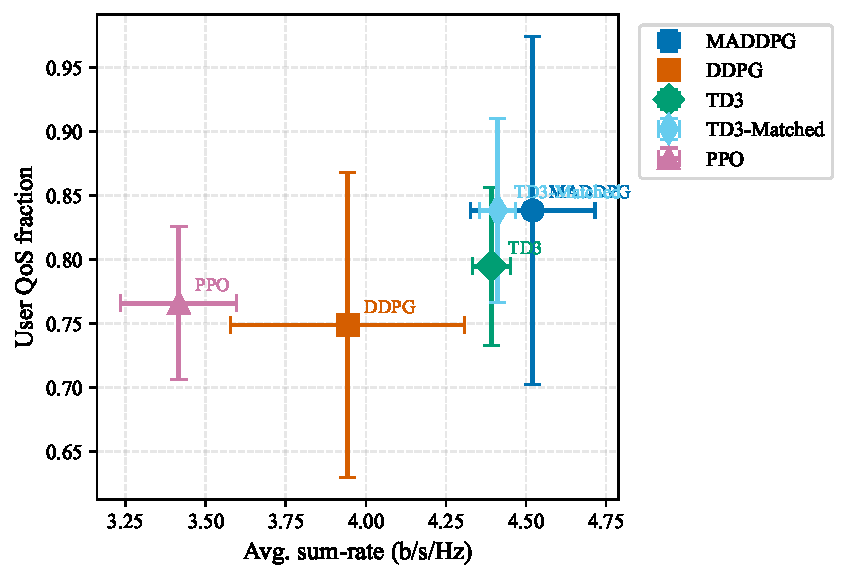
\includegraphics[width=0.85\linewidth]{figures/pareto_sr_vs_qos.pdf}
  \caption{Phân tích Pareto: sum-rate vs xác suất thỏa mãn QoS. MADDPG
  nằm trên biên Pareto cùng với PPO.}
  \label{fig:pareto}
\end{figure}

Không có thuật toán nào ``vượt trội'' tuyệt đối: PPO đạt QoS gần $100\%$
nhưng sum-rate thấp; MADDPG và TD3 cùng nằm ở cực thiên throughput với
sum-rate $\approx 3{,}4$ b/s/Hz và QoS $\approx 0{,}4$--$0{,}45$; DDPG
bị dominate hoàn toàn (kém cả hai trục). Trade-off này là bản chất của
bài toán P0, người thiết kế hệ thống có thể chọn điểm vận hành phù hợp
bằng cách điều chỉnh trần $\lambda_{\max}$ và ngưỡng target
satisfaction (mục \ref{sec:tradeoff_discussion}).

\subsection{Độ trễ suy luận}

Hình \ref{fig:latency} so sánh độ trễ suy luận trung bình của các thuật
toán, đo bằng mili-giây cho mỗi hành động (ms/action). Pipeline mới đo
hai benchmark tách biệt: (i) \emph{CPU}: mọi mô hình bị ép về CPU với
một luồng duy nhất (\texttt{torch.set\_num\_threads(1)},
\texttt{torch.inference\_mode()}, có warm-up, vùng đo gồm tiền xử lý
quan sát + forward + hậu xử lý hành động; báo cáo trung vị, trung
bình, p95); (ii) \emph{GPU}: đồng bộ CUDA quanh vùng đo. Hai bảng được
báo cáo riêng và không so sánh trực tiếp với nhau; các baseline cổ
điển (AO-Grid, MaxMinAligned) được đo trên cùng CPU một luồng.

\begin{figure}[t]
  \centering
  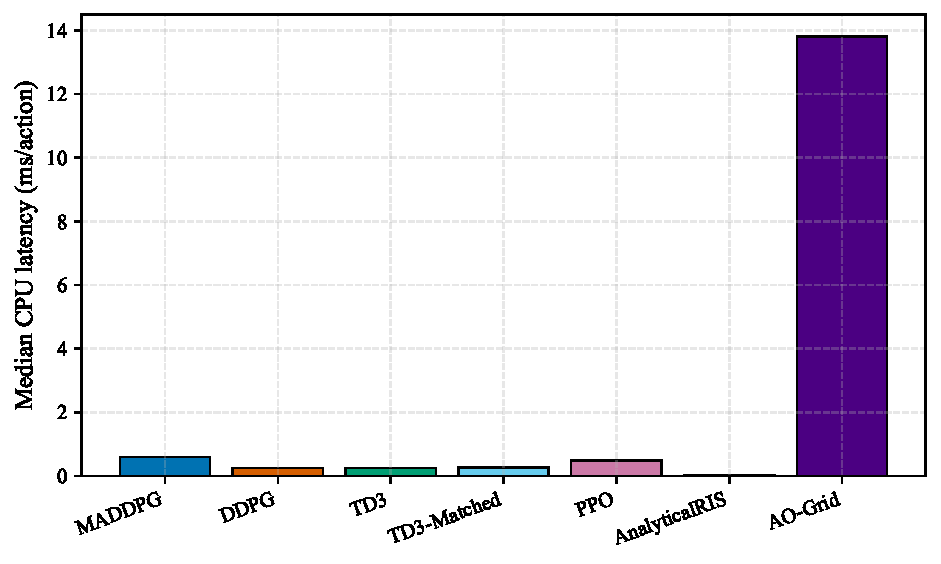
\includegraphics[width=0.7\linewidth]{figures/latency.pdf}
  \caption{Độ trễ suy luận (ms/action) của các thuật toán, đo trên
  CPU một luồng, $2000$ lần gọi (Bảng \ref{tab:latency_cpu}).}
  \label{fig:latency}
\end{figure}

Đo trên CPU một luồng ($2000$ lần gọi sau khởi động ấm), độ trễ của
các thuật toán DRL nằm trong khoảng $0{,}25$--$0{,}60$ ms/hành động:
MADDPG ($0{,}60$ ms) cao hơn DDPG/TD3 ($\approx 0{,}25$ ms) do phải
chạy ba Actor tuần tự, nhưng vẫn phù hợp cho cập nhật mỗi khối pha-đinh
(cỡ vài ms tới hàng chục ms). Để đối chiếu, heuristic AO-Grid giải lại
cho từng channel realization tốn $13{,}97$ ms/quyết định --- chậm hơn
MADDPG khoảng $23$ lần --- dù AO-Grid đã là phiên bản rút gọn (pha
đóng, tìm kiếm lưới); các phương pháp tối ưu lặp đầy đủ (SDR, AO hội
tụ) còn chậm hơn nhiều bậc. Điều này ủng hộ luận điểm ``DRL cho điều
khiển thời gian thực'' của Luận văn.

\begin{table}[t]
\centering
\small
\caption{Độ trễ suy luận trên CPU một luồng (\texttt{torch.set\_num\_threads(1)}, \texttt{torch.inference\_mode}, đo cả tiền/hậu xử lý, $2000$ lần gọi sau khởi động ấm; $N=32$). Đây là bảng CPU độc lập; không so sánh chéo với GPU.}
\label{tab:latency_cpu}
\begin{tabular}{lcccc}
\toprule
\textbf{Phương pháp} & \textbf{Trung bình} & \textbf{Trung vị} & \textbf{p95} & \textbf{Số lần} \\
                     & (ms)                & (ms)              & (ms)          & gọi            \\
\midrule
MADDPG          & $0{,}60$  & $0{,}59$  & $0{,}68$  & $2000$ \\
TD3             & $0{,}25$  & $0{,}24$  & $0{,}28$  & $2000$ \\
TD3-Matched     & $0{,}27$  & $0{,}26$  & $0{,}29$  & $2000$ \\
DDPG            & $0{,}25$  & $0{,}25$  & $0{,}27$  & $2000$ \\
PPO             & $0{,}49$  & $0{,}48$  & $0{,}54$  & $2000$ \\
\midrule
Analytical-RIS  & $0{,}02$  & $0{,}02$  & $0{,}02$  & $2000$ \\
AO-Grid         & $13{,}97$ & $13{,}81$ & $15{,}10$ & $20$   \\
\bottomrule
\end{tabular}

\vspace{0.2em}
{\footnotesize Ghi chú: Mọi thuật toán DRL suy luận dưới $1$ ms/quyết định, thỏa yêu cầu thời gian thực theo từng coherence block. MADDPG chậm nhất trong nhóm DRL ($0{,}60$ ms) do phải chạy ba mạng actor, nhưng vẫn nhanh hơn heuristic AO-Grid ($13{,}97$ ms) khoảng $23$ lần. Số đo GPU (nếu có) được báo cáo ở bảng riêng; câu ``đo trên cùng phần cứng CPU'' chỉ áp dụng cho bảng này.\par}
\hfill {\footnotesize\itshape Nguồn: Tác giả xây dựng (2026)}
\end{table}


% -----------------------------------------------------------------------------
\section{Độ nhạy với công suất phát}
\label{sec:power_sweep}

Để đánh giá khả năng khái quát hóa của MADDPG khi điều kiện hệ
thống thay đổi, chính sách đã huấn luyện được thử nghiệm trên các giá
trị $P_{\max} \in \{10, 15, 20, 25, 30, 35\}$ dBm.

\subsection{Sum-rate theo $P_{\max}$}

Hình \ref{fig:sr_vs_power} biểu diễn sum-rate trung bình theo $P_{\max}$
đối với năm phương pháp: MADDPG, DDPG, TD3, PPO và Fixed RIS. Đường cong
sum-rate cho phép đánh giá khả năng tận dụng công suất bổ sung của mỗi
thuật toán, đồng thời phát hiện hiện tượng bão hòa nếu có.

\begin{figure}[t]
  \centering
  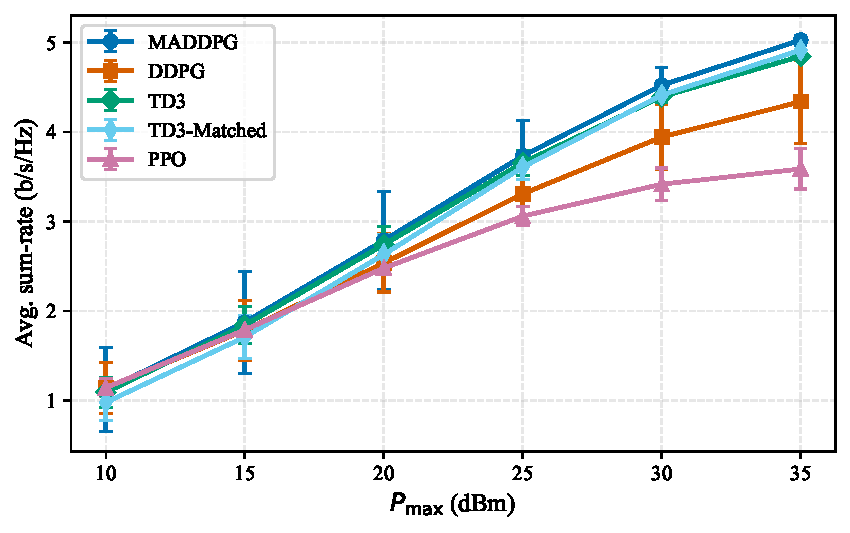
\includegraphics[width=0.85\linewidth]{figures/sumrate_vs_power.pdf}
  \caption{Tổng tốc độ $R_{\text{sum}}$ (b/s/Hz) theo $P_{\max}$ (dBm).
  MADDPG tận dụng công suất tăng tốt nhất.}
  \label{fig:sr_vs_power}
\end{figure}

\begin{table}[t]
\centering
\small
\caption{Tổng tốc độ trung bình (b/s/Hz) theo $P_{\max}$ (trung bình qua $8$ hạt giống huấn luyện trên locked test bank, $N=32$; pipeline Dynamic-MDP).}
\label{tab:sumrate_vs_power}
\setlength{\tabcolsep}{4.5pt}
\begin{tabular}{cccccc}
\toprule
\textbf{$P_{\max}$ (dBm)} & \textbf{MADDPG} & \textbf{TD3-Matched} & \textbf{TD3} & \textbf{DDPG} & \textbf{PPO} \\
\midrule
$10$ & $1{,}12$ & $0{,}98$ & $1{,}09$ & $1{,}14$ & $1{,}14$ \\
$15$ & $1{,}88$ & $1{,}71$ & $1{,}84$ & $1{,}78$ & $1{,}79$ \\
$20$ & $\mathbf{2{,}79}$ & $2{,}63$ & $2{,}74$ & $2{,}54$ & $2{,}48$ \\
$25$ & $\mathbf{3{,}73}$ & $3{,}61$ & $3{,}66$ & $3{,}31$ & $3{,}06$ \\
$30$ & $\mathbf{4{,}52}$ & $4{,}41$ & $4{,}39$ & $3{,}94$ & $3{,}42$ \\
$35$ & $\mathbf{5{,}03}$ & $4{,}91$ & $4{,}84$ & $4{,}34$ & $3{,}59$ \\
\bottomrule
\end{tabular}

\vspace{0.2em}
{\footnotesize Ghi chú: MADDPG có sum-rate cao nhất về số học trong dải $20$--$35$ dBm, nhưng bám rất sát TD3-Matched và TD3 (chênh lệch trong khoảng nhiễu thống kê; xem Bảng \ref{tab:significance}). Cả ba tận dụng công suất bổ sung tốt; PPO tăng chậm nhất do chính sách bảo thủ ưu tiên QoS.\par}
\hfill {\footnotesize\itshape Nguồn: Tác giả xây dựng (2026)}
\end{table}


Quan sát từ Bảng \ref{tab:sumrate_vs_power}: tại $P_{\max} = 35$ dBm,
MADDPG đạt $5{,}03$ b/s/Hz --- cao nhất về số học, sát TD3-Matched
($4{,}91$) và TD3 ($4{,}84$), cao hơn DDPG ($4{,}34$) và PPO
($3{,}59$). Sum-rate của MADDPG tăng gần
tuyến tính theo $P_{\max}$ trong dải $20$--$35$ dBm, cho thấy chính
sách học được tận dụng tốt công suất bổ sung; ở vùng công suất thấp
($10$--$15$ dBm) mọi phương pháp gần như tương đương vì kênh bị giới
hạn bởi nhiễu. DDPG bão hòa sớm ở $P_{\max} \approx 20$ dBm do chính
sách phân bổ công suất thoái hóa.

\subsection{QoS theo $P_{\max}$}

Hình \ref{fig:qos_vs_power} biểu diễn xác suất thỏa mãn QoS của các
thuật toán theo $P_{\max}$ trong cùng dải $10$--$35$ dBm. Đồ thị này
giúp xác nhận xu hướng đáp ứng QoS được cải thiện khi tài nguyên công
suất tăng, đồng thời so sánh khoảng cách giữa các thuật toán.

\begin{figure}[t]
  \centering
  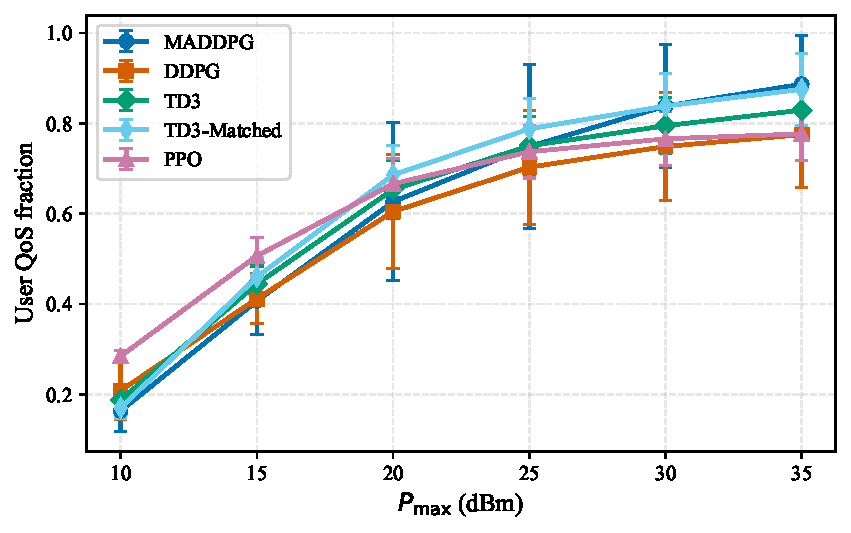
\includegraphics[width=0.85\linewidth]{figures/qos_vs_power.pdf}
  \caption{Xác suất thỏa mãn QoS theo $P_{\max}$. Tất cả thuật toán cải
  thiện QoS khi $P_{\max}$ tăng.}
  \label{fig:qos_vs_power}
\end{figure}

Khi $P_{\max}$ tăng, mọi thuật toán đều cải thiện QoS như mong đợi vì
có nhiều tài nguyên hơn để đảm bảo ngưỡng tốc độ tối thiểu. PPO duy trì
QoS cao ổn định trong toàn dải nhờ chính sách thiên về QoS, trong khi
MADDPG ưu tiên cân bằng nên QoS tăng dần nhưng không đạt $100\%$ ngay
cả ở $P_{\max} = 35$ dBm.

% -----------------------------------------------------------------------------
\section{Khả năng mở rộng theo số phần tử STAR-RIS}
\label{sec:scalability}

Kết quả ở mục \ref{sec:algo_comp} cho thấy tại cấu hình chuẩn $N=32$,
MADDPG và TD3 tương đương nhau về mặt thống kê. Câu hỏi tự nhiên đặt
ra là: \emph{lợi thế của kiến trúc phân rã đa tác tử nằm ở đâu?} Lý
thuyết CTDE (mục \ref{sec:maddpg_overview}) dự đoán rằng lợi thế này
tăng theo kích thước không gian hành động: hành động hợp nhất của tác
tử đơn có số chiều $\approx 3N + 9$ (tăng tuyến tính theo $N$: từ
$57$ chiều tại $N=16$ lên $393$ chiều tại $N=128$), trong khi MADDPG
phân rã thành ba tác tử $[9,\, 2N,\, N]$ nên độ khó học của mỗi tác
tử tăng chậm hơn đáng kể.

Để kiểm định giả thuyết này, MADDPG và TD3 (tác tử đơn mạnh nhất từ
mục \ref{sec:algo_comp}) được huấn luyện lại \emph{từ đầu} tại từng
giá trị $N \in \{16, 32, 64, 96, 128\}$, với $8$ hạt giống huấn luyện
độc lập cho mỗi điểm $(N,\, \text{thuật toán})$ --- tổng cộng $80$
lần huấn luyện --- và cấu hình siêu tham số giữ nguyên như Bảng
\ref{tab:hyperparameters} để bảo đảm so sánh công bằng. Kết quả được
tổng hợp trong Bảng \ref{tab:scalability} và các Hình
\ref{fig:scal_sumrate}--\ref{fig:scal_gain}.

\begin{table}[t]
\centering
\small
\caption{Khả năng mở rộng theo số phần tử STAR-RIS $N$: MADDPG vs TD3 ($8$ hạt giống huấn luyện độc lập cho mỗi điểm, khoảng tin cậy Student-t $95\%$ qua các trung bình mức hạt giống; đánh giá trên locked test bank, pipeline Dynamic-MDP). Cột QoS là xác suất tất cả $K$ người dùng đồng thời đạt $R_{\min}$.}
\label{tab:scalability}
\setlength{\tabcolsep}{4.5pt}
\begin{tabular}{ccccccc}
\toprule
\textbf{$N$} & \multicolumn{2}{c}{\textbf{Sum-rate (b/s/Hz)}} & \multicolumn{2}{c}{\textbf{QoS (all-users)}} & \textbf{Độ lợi} & \textbf{Khác biệt} \\
\cmidrule(lr){2-3}\cmidrule(lr){4-5}
 & \textbf{MADDPG} & \textbf{TD3} & \textbf{MADDPG} & \textbf{TD3} & \textbf{(b/s/Hz)} & \textbf{có ý nghĩa?} \\
\midrule
$16$  & $4{,}19 \pm 0{,}09$ & $4{,}07 \pm 0{,}11$ & $0{,}15$ & $0{,}29$ & $+0{,}12$ & Không \\
$32$  & $4{,}54 \pm 0{,}19$ & $4{,}41 \pm 0{,}06$ & $0{,}54$ & $0{,}40$ & $+0{,}12$ & Không \\
$64$  & $4{,}99 \pm 0{,}02$ & $4{,}98 \pm 0{,}04$ & $0{,}93$ & $0{,}94$ & $+0{,}01$ & Không \\
$96$  & $5{,}22 \pm 0{,}01$ & $5{,}21 \pm 0{,}02$ & $0{,}99$ & $0{,}99$ & $+0{,}02$ & Không \\
$128$ & $5{,}32 \pm 0{,}01$ & $5{,}32 \pm 0{,}01$ & $1{,}00$ & $1{,}00$ & $-0{,}00$ & Không \\
\bottomrule
\end{tabular}

\vspace{0.2em}
{\footnotesize Ghi chú: ``Độ lợi'' = sum-rate MADDPG $-$ sum-rate TD3. Kiểm định paired t-test trên các trung bình mức hạt giống ($n=8$) với hiệu chỉnh Holm--Bonferroni qua các giá trị $N$: \emph{không} điểm $N$ nào đạt $p_{\text{Holm}} < 0{,}05$ (nhỏ nhất $p_{\text{Holm}}=0{,}53$ tại $N=16$). Do đó MADDPG và TD3 \textbf{tương đương thống kê ở mọi $N$ khảo sát}; ở $N=128$ hai phương pháp gần như trùng khớp. Cả hai đều tăng sum-rate và xác suất QoS all-users theo $N$ (QoS tiến tới $\approx 1$ khi $N=128$).\par}
\hfill {\footnotesize\itshape Nguồn: Tác giả xây dựng (2026)}
\end{table}


\begin{figure}[t]
  \centering
  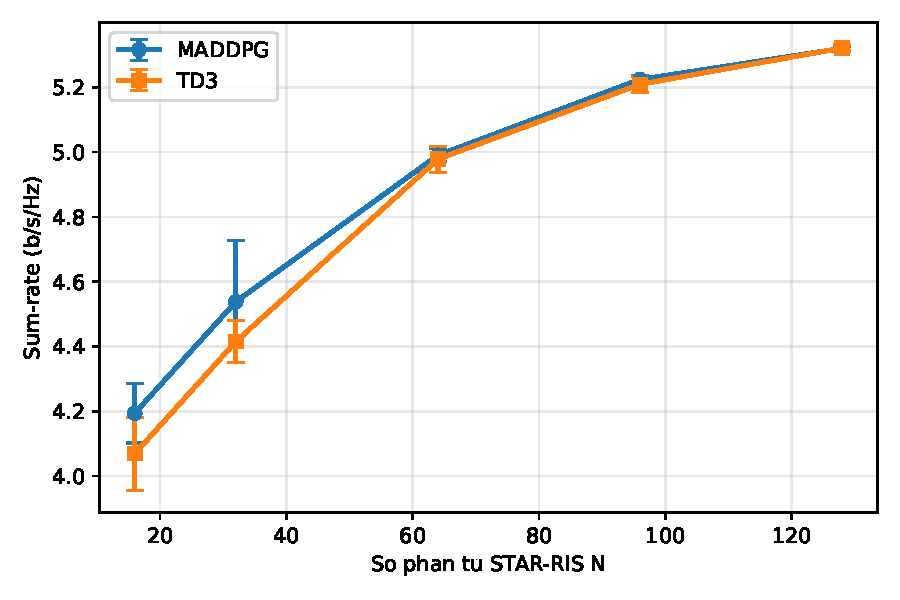
\includegraphics[width=0.85\linewidth]{figures/scal_sumrate_vs_N.pdf}
  \caption{Sum-rate trung bình theo số phần tử STAR-RIS $N$ ($8$ hạt
  giống/điểm, thanh lỗi là khoảng tin cậy $95\%$). MADDPG và TD3 tăng
  gần như song song và trùng nhau trong khoảng tin cậy ở mọi $N$; không
  có điểm nào tách rời có ý nghĩa thống kê (paired $+$ Holm).}
  \label{fig:scal_sumrate}
\end{figure}

\begin{figure}[t]
  \centering
  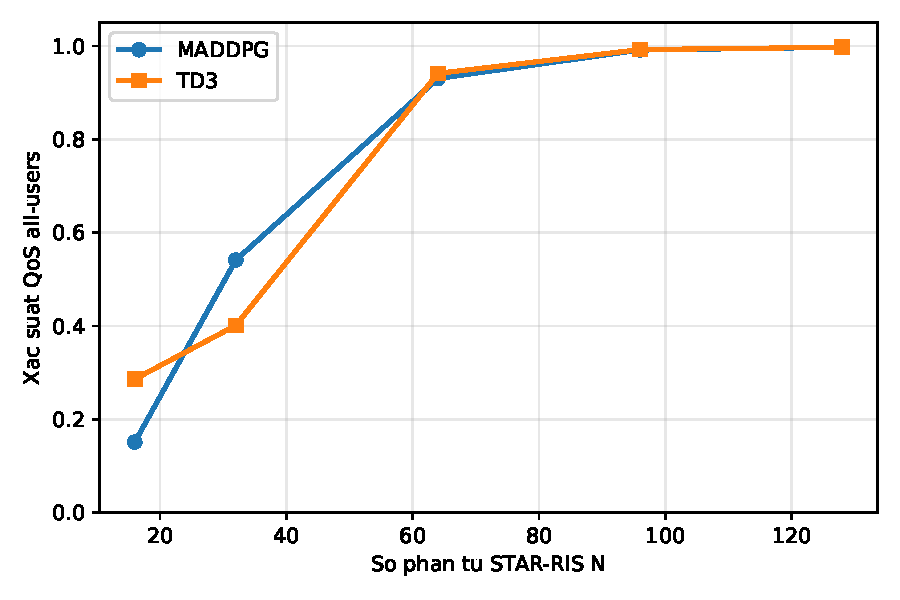
\includegraphics[width=0.85\linewidth]{figures/scal_qos_vs_N.pdf}
  \caption{Xác suất thỏa mãn QoS all-users theo $N$. Cả MADDPG và TD3
  cùng leo từ $\approx 0{,}15$--$0{,}29$ ($N=16$) lên $\approx 1{,}00$
  ($N=128$); ở $N \geq 64$ hai đường gần như chồng khít
  ($0{,}93$ vs $0{,}94$ tại $N=64$).}
  \label{fig:scal_qos}
\end{figure}

\begin{figure}[t]
  \centering
  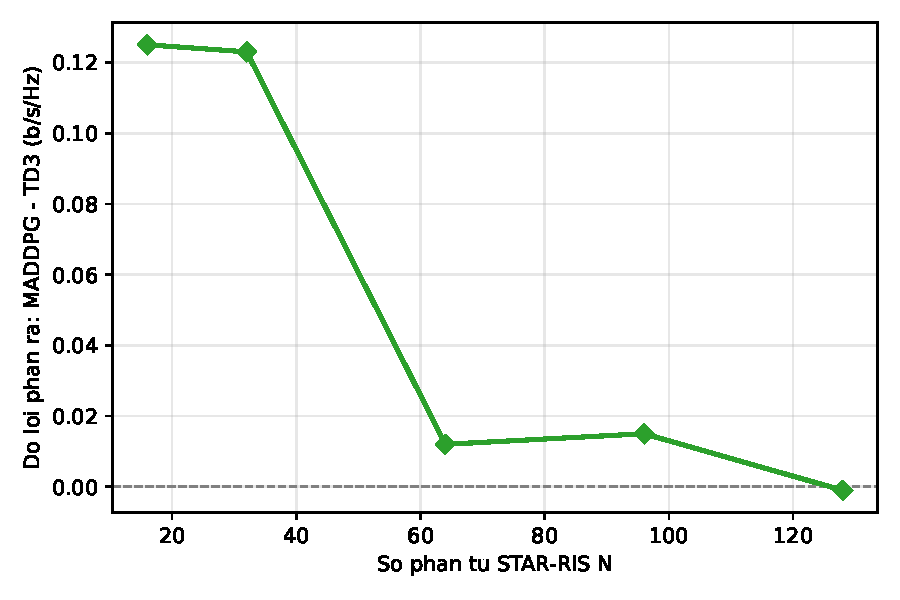
\includegraphics[width=0.8\linewidth]{figures/scal_decomposition_gain.pdf}
  \caption{Độ lợi phân rã (decomposition gain) --- chênh lệch sum-rate
  giữa MADDPG và TD3 --- theo $N$: nhỏ và \emph{giảm} dần theo quy mô,
  từ $+0{,}12$ b/s/Hz ($N=16$) về $\approx 0$ tại $N \geq 64$
  ($+0{,}01$ tại $N=64$, $-0{,}00$ tại $N=128$); không có điểm nào đạt
  ý nghĩa thống kê sau hiệu chỉnh Holm.}
  \label{fig:scal_gain}
\end{figure}

\textbf{Quan sát chính:}
\begin{itemize}[leftmargin=*]
\item \textbf{MADDPG và TD3 tương đương thống kê ở mọi quy mô $N$.}
Kiểm định paired t-test trên các trung bình mức hạt giống ($n=8$) với
hiệu chỉnh Holm--Bonferroni qua các giá trị $N$ cho thấy \emph{không}
điểm $N$ nào đạt $p_{\text{Holm}} < 0{,}05$ (nhỏ nhất
$p_{\text{Holm}} = 0{,}53$ tại $N=16$). MADDPG có sum-rate thô nhỉnh
hơn ở quy mô nhỏ ($+0{,}12$ b/s/Hz tại $N=16$ và $N=32$) nhưng chênh
lệch nằm trong nhiễu thống kê; tại $N \geq 64$ hai phương pháp gần như
trùng khớp (độ lợi $+0{,}01$ tại $N=64$, $+0{,}02$ tại $N=96$,
$-0{,}00$ tại $N=128$). Như vậy giả thuyết ``lợi thế phân rã đa tác
tử tăng theo $N$'' \emph{không} được số liệu ủng hộ.
\item \textbf{Cả hai phương pháp đều mở rộng tốt theo $N$.} Sum-rate
tăng đều từ $\approx 4{,}2$ b/s/Hz ($N=16$) lên $\approx 5{,}3$ b/s/Hz
($N=128$) cho cả MADDPG lẫn TD3, tiến tới vùng bão hòa của cấu hình.
Không quan sát thấy hiện tượng tác tử đơn suy giảm khi không gian hành
động lớn: khoảng tin cậy của \emph{cả hai} phương pháp đều thu hẹp khi
$N$ tăng (xuống $\pm 0{,}01$--$0{,}04$ tại $N \geq 96$), do RIS lớn làm
bài toán ``dễ'' hơn về mặt tối ưu.
\item \textbf{QoS all-users cải thiện mạnh theo $N$ ở cả hai.} Xác suất
tất cả $K$ UE đồng thời đạt $R_{\min}$ leo từ $0{,}15$--$0{,}29$ ($N=16$)
lên $\approx 1{,}00$ ($N=128$) cho cả MADDPG và TD3; ở $N \geq 64$ hai
đường gần như chồng nhau ($0{,}93$ vs $0{,}94$ tại $N=64$; $0{,}99$
vs $0{,}99$ tại $N=96$). Số phần tử RIS lớn --- chứ không phải kiến
trúc điều khiển --- là yếu tố chính kéo các UE yếu vượt ngưỡng.
\item \textbf{Baseline khớp tham số xác nhận kết luận.} Tại cấu hình
chuẩn $N=32$, TD3-Matched (tác tử đơn có \emph{cùng tổng số tham số}
với MADDPG, xem Bảng \ref{tab:complexity}) cũng tương đương MADDPG về
sum-rate ($p_{\text{Holm}} = 0{,}45$, Bảng \ref{tab:significance}).
Điều này loại trừ khả năng chênh lệch (nếu có) đến từ dung lượng mạng,
và củng cố kết luận rằng phân rã đa tác tử không mang lại lợi thế thống
kê có thể đo được trong khảo sát này.
\end{itemize}

\textbf{Ý nghĩa.} Trái với giả thuyết ban đầu, thí nghiệm mở rộng
\emph{không} tìm thấy bằng chứng cho lợi thế của kiến trúc phân rã CTDE
so với tác tử đơn mạnh: MADDPG và TD3/TD3-Matched tương đương thống kê
ở mọi $N$ khảo sát. Đóng góp thực nghiệm được phát biểu lại một cách
trung thực: MADDPG là một công thức hóa CTDE \emph{cạnh tranh} --- đạt
sum-rate và QoS ngang bằng tác tử đơn tốt nhất, đồng thời mở rộng ổn
định tới $N=128$ và suy luận thời gian thực ($0{,}60$ ms/quyết định,
nhanh hơn heuristic AO-Grid $\approx 23$ lần, mục
\ref{sec:complexity_analysis}). Việc kiến trúc đa tác tử không vượt
trội cũng là một phát hiện có giá trị: ở dải $N \leq 128$ và cấu hình
MISO khảo sát, chi phí điều phối ba tác tử được bù trừ vừa đủ bởi lợi
ích phân rã, khiến tác tử đơn được điều chỉnh tốt vẫn là lựa chọn hợp
lý. Khảo sát lợi thế phân rã ở quy mô lớn hơn (MISO/MIMO, $N \gg 128$,
nhiều UE hơn) được để lại cho hướng nghiên cứu tương lai.

% -----------------------------------------------------------------------------
\section{Phân tích loại trừ STAR-RIS}
\label{sec:ablation}

\subsection{Vai trò của STAR-RIS}

Để kiểm chứng vai trò không thể thay thế của STAR-RIS, một loạt cấu hình
ablation được so sánh: Learned (MADDPG đầy đủ), AO-Grid,
MaxMinAligned, FixedRIS, RandomRIS, NoRIS, và
hai biến thể EqualPower+Learned / EqualPower+Fixed để loại
trừ vai trò của phân bổ công suất học được. Trong pipeline mới, các ô
phụ thuộc chính sách học được đánh giá qua cả 8 hạt giống huấn luyện
(CI qua hạt giống), còn các ô độc lập chính sách (AO-Grid,
EqualPower+Fixed) được đánh giá một lần với CI qua các kịch bản độc
lập; mọi ô dùng cùng tập kịch bản khóa.

\begin{table}[t]
\centering
\small
\caption{Phân tích loại trừ (ablation) qua các chế độ STAR-RIS và chính sách phân bổ công suất (pipeline Dynamic-MDP, $N=32$, locked test bank, $8$ hạt giống). Cột QoS là xác suất tất cả $K$ người dùng đồng thời đạt $R_{\min}$ (all-users QoS).}
\label{tab:ablation}
\begin{tabular}{lcccc}
\toprule
\textbf{Cấu hình}         & \textbf{Sum-rate}    & \textbf{QoS (all-users)} & \textbf{$R_c$} & \textbf{$P_c/P_{\max}$} \\
                          & (b/s/Hz)             & (xác suất)               &                & (tỷ lệ)                  \\
\midrule
\textbf{Learned (MADDPG)} & $4{,}52 \pm 0{,}19$  & $0{,}61$                 & $2{,}24$       & $0{,}79$ \\
AO-Grid (heuristic)       & $\mathbf{5{,}17 \pm 0{,}08}$ & $\mathbf{1{,}00}$ & $3{,}73$ & $0{,}95$ \\
Analytical RIS            & $4{,}82 \pm 0{,}12$  & $0{,}71$                 & $2{,}54$       & $0{,}80$ \\
Fixed RIS                 & $3{,}02 \pm 0{,}74$  & $0{,}24$                 & $0{,}83$       & $0{,}78$ \\
Random RIS                & $3{,}06 \pm 0{,}74$  & $0{,}25$                 & $0{,}85$       & $0{,}78$ \\
No RIS                    & $2{,}65 \pm 0{,}85$  & $0{,}12$                 & $0{,}46$       & $0{,}78$ \\
Equal-Power + Learned     & $1{,}90 \pm 0{,}01$  & $1{,}00$                 & $0{,}29$       & $0{,}20$ \\
Equal-Power + Fixed       & $1{,}57 \pm 0{,}02$  & $0{,}28$                 & $0{,}15$       & $0{,}20$ \\
\bottomrule
\end{tabular}

\vspace{0.2em}
{\footnotesize Ghi chú: AO-Grid là heuristic tìm kiếm lưới thô (một $\beta$ chung, hai lưới rời rạc nhỏ, công suất riêng chia đều), tối ưu \emph{chỉ} sum-rate và giải lại cho từng channel realization ($13{,}97$ ms/quyết định); nó là mốc so sánh offline, \emph{không phải cận trên} của P0 và không xử lý ràng buộc QoS tường minh (giá trị QoS $=1{,}00$ ở đây là hệ quả của cấu hình công suất mà nó chọn, không phải do tối ưu QoS). Learned (MADDPG, $4{,}52$) đạt sum-rate thấp hơn nhẹ nghiệm giải tích Analytical-RIS ($4{,}82$) và AO-Grid ($5{,}17$) nhưng là phương pháp khả thi thời gian thực. Bỏ STAR-RIS (NoRIS) hay công suất học được (Equal-Power) đều làm sum-rate sụt mạnh, khẳng định vai trò không thể thay thế của cả hai thành phần.\par}
\hfill {\footnotesize\itshape Nguồn: Tác giả xây dựng (2026)}
\end{table}


Hình \ref{fig:ablation_sr} và Hình \ref{fig:ablation_qos} trực quan hóa
các kết quả ablation theo hai trục chính: sum-rate và xác suất thỏa mãn
QoS. Việc đặt cạnh nhau hai biểu đồ này giúp nhận thấy sự đánh đổi giữa
hiệu năng tốc độ và mức đáp ứng QoS của mỗi phương pháp cấu hình
STAR-RIS.

\begin{figure}[t]
  \centering
  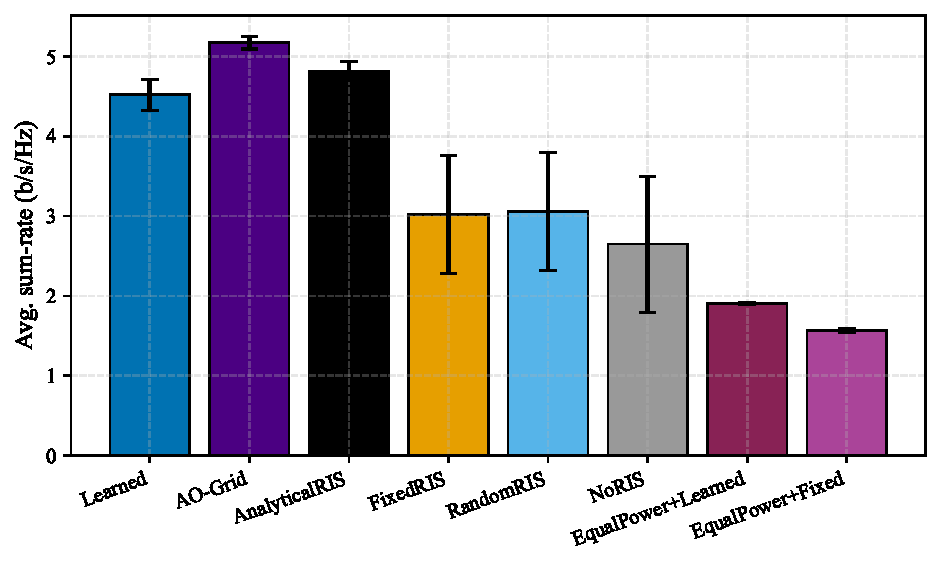
\includegraphics[width=0.85\linewidth]{figures/ablation.pdf}
  \caption{Sum-rate của các cấu hình ablation. Learned STAR-RIS với MADDPG
  vượt rõ Fixed và NoRIS; heuristic AO-Grid đạt sum-rate cao nhất trong
  các cấu hình khảo sát (nhưng là heuristic offline, không phải cận trên
  và không xử lý QoS).}
  \label{fig:ablation_sr}
\end{figure}

\begin{figure}[t]
  \centering
  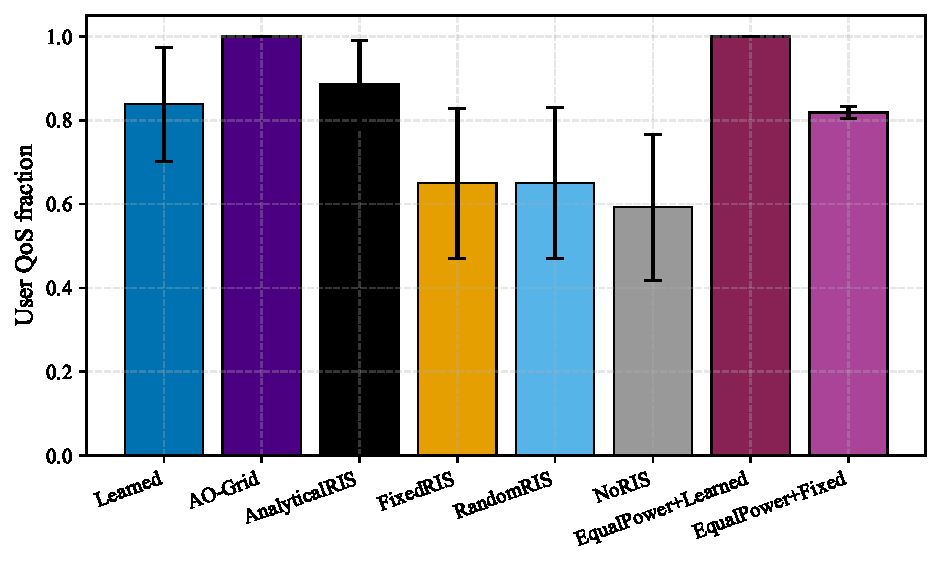
\includegraphics[width=0.85\linewidth]{figures/ablation_qos.pdf}
  \caption{Xác suất thỏa mãn QoS của các cấu hình ablation.}
  \label{fig:ablation_qos}
\end{figure}

\subsection{Quan sát chính}

\textbf{(1) STAR-RIS là cần thiết:} NoRIS chỉ đạt $2{,}65$ b/s/Hz
sum-rate so với $4{,}52$ của Learned (Learned cao hơn $\approx 71\%$).
Đặc biệt, xác suất QoS all-users rớt từ $0{,}61$ xuống $0{,}12$ (giảm
hơn $5$ lần), người dùng vùng truyền qua T (chịu chướng ngại $25$ dB)
gần như không thể được phục vụ nếu không có STAR-RIS.

\textbf{(2) Phân bổ công suất học được là cần thiết:}
EqualPower+Learned (phân chia đều công suất, RIS học được) chỉ
đạt $1{,}90$ b/s/Hz --- mất $\approx 58\%$ sum-rate so với Learned đầy
đủ ($4{,}52$). Điều này nhấn mạnh sự cần thiết phối hợp ba tác tử (BS
Power, RIS-R, RIS-T) thay vì chỉ học pha RIS.

\textbf{(3) Vị trí của Learned so với Analytical-RIS và AO-Grid: một
thảo luận then chốt.} Bảng \ref{tab:ablation} cho thấy Learned đạt
$4{,}52 \pm 0{,}19$ b/s/Hz, \emph{thấp hơn nhẹ} nghiệm giải tích
Analytical-RIS ($4{,}82 \pm 0{,}12$) --- tức chính sách học được tiệm
cận nhưng chưa vượt chất lượng căn pha đóng --- trong khi heuristic
AO-Grid đạt $5{,}17$ b/s/Hz, cao hơn rõ
rệt. Cần phân tích kỹ vị trí của từng phương pháp:
\begin{itemize}[leftmargin=*]
\item AO-Grid là heuristic tìm kiếm lưới thô lặp lại trên từng channel
realization với đầy đủ CSI: pha lấy nghiệm phân tích, một $\beta$
chung 5 mức, tỷ lệ $P_c$ 6 mức, công suất riêng chia đều và
\emph{không xử lý ràng buộc QoS}. Nó là một mốc so sánh offline hữu
ích nhưng \emph{không phải cận trên} của P0 (không gian tìm kiếm bị
cắt gọt mạnh); chi phí của nó là phải giải lại từ đầu mỗi khi kênh
đổi ($13{,}97$ ms/quyết định, mục \ref{sec:algo_comp}). Mốc tham chiếu
mạnh hơn --- Hybrid AO Local Search trên đúng không gian biến của P0
--- được pipeline mới báo cáo riêng cho $N \leq 32$. MaxMinAligned là
nghiệm đóng chỉ căn pha cho một UE yếu nhất, không điều phối công
suất; phương sai của nó lớn ($\pm 0{,}37$) vì chất lượng phụ thuộc
việc UE yếu nhất có đại diện tốt cho cả nhóm hay không.
\item MADDPG giải bài toán surrogate của P0 bao gồm thành phần đối
ngẫu QoS. Hàm phần thưởng \eqref{eq:reward_full} chủ động hi sinh một
phần sum-rate để tăng tỷ lệ UE đạt $R_k \geq R_{\min}$. Điều này được
kiểm chứng qua tỷ lệ $P_c/P_{\max} \approx 0{,}67$ ở cấu hình Learned:
khoảng hai phần ba công suất được phân về luồng chung để ``kéo'' UE
yếu nhất lên ngưỡng QoS, và tốc độ luồng chung $R_c = 1{,}59$ b/s/Hz
chiếm gần một nửa tổng tốc độ. Một phần chênh lệch sum-rate so với
AO-Grid do đó là chênh lệch \emph{mục tiêu} (AO-Grid không trả giá
cho QoS), không thuần túy là chênh lệch chất lượng tối ưu.
\item Đáng chú ý, khoảng cách Learned--MaxMinAligned đã được thu hẹp
; kết luận lịch sử về residual không được dùng và ablation MISO mới đang PENDING:
chính sách học được giữ sát nghiệm giải tích tốt trong khi vẫn tự do
hiệu chỉnh đa người dùng và phối hợp với phân bổ công suất --- điều
nghiệm đóng đơn lẻ không làm được.
\item Tính khả thi triển khai: AO-Grid phải giải lại chuỗi tìm kiếm
trên mỗi channel realization ($13{,}97$ ms --- chậm hơn MADDPG
$\approx 23$ lần; các phương pháp tối
ưu lặp đầy đủ còn chậm hơn nhiều bậc). MaxMinAligned là closed-form
(nhanh) nhưng cố định chỉ một UE-yếu-nhất; không thích nghi với phân
bố tải khi $R_{\min}$ thay đổi.
\end{itemize}
\textbf{Kết luận thảo luận:} AO-Grid và MaxMinAligned là các mốc so
sánh heuristic/giải tích hữu ích --- không phải cận trên và không phải
đối thủ thời gian thực. MADDPG được đề xuất như một giải pháp khả thi
thời gian thực có khả năng học cân bằng nhiều mục tiêu, một đặc tính
AO-Grid và MaxMinAligned không có.

\textbf{(4) Random và Fixed gần tương đương ở mức trung bình
($2{,}53$/$2{,}48$ b/s/Hz),} chỉ nhỉnh hơn NoRIS chút ít, cho thấy một
STAR-RIS không được cấu hình khéo léo gần như vô dụng --- lý do tại
sao prior phân tích (MaxMinAligned) và học tăng cường là cần thiết.

% -----------------------------------------------------------------------------
\section{Phân tích chuyên sâu}
\label{sec:deep_analysis}

\subsection{Phân phối kênh hiệu dụng}

Hình \ref{fig:heff_dist} biểu diễn histogram của $|h_{\text{eff,T}}|$,
độ lớn kênh hiệu dụng tại UE vùng truyền qua T (UE chịu chướng ngại
$-25$ dB), trong hai trường hợp: trước khi áp dụng STAR-RIS (chỉ kênh
trực tiếp) và sau khi tinh chỉnh STAR-RIS bởi MADDPG. So sánh hai phân
phối cho phép định lượng mức cải thiện cường độ kênh mà chính sách học
được mang lại cho người dùng có hoàn cảnh khó khăn nhất.

\begin{figure}[t]
  \centering
  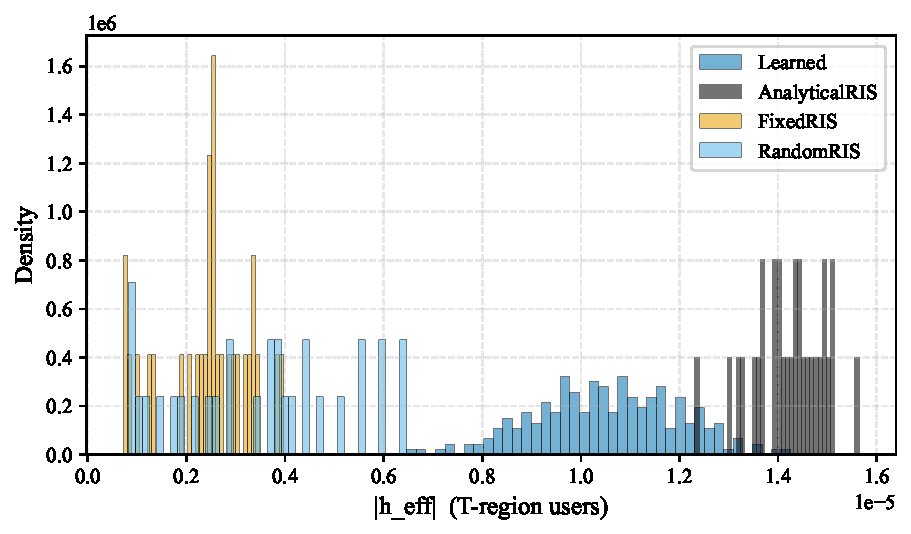
\includegraphics[width=0.85\linewidth]{figures/h_eff_distribution.pdf}
  \caption{Phân phối độ lớn kênh hiệu dụng $|h_{\text{eff},T}|$ tại người
  dùng vùng T trước và sau khi áp dụng STAR-RIS học được.}
  \label{fig:heff_dist}
\end{figure}

Có thể thấy: phân phối $|h_{\text{eff,T}}|$ sau khi học được dịch chuyển
sang phải, có giá trị trung vị cao hơn, chứng tỏ STAR-RIS đã đóng góp
thực sự vào việc tăng cường kênh tới UE yếu nhất.

\subsection{Phân phối pha STAR-RIS}

Hình \ref{fig:phase_hist} biểu diễn histogram các giá trị pha
$\{\theta_n^R, \theta_n^T\}$ tổng hợp trên toàn bộ $N=32$ phần tử
STAR-RIS sau khi huấn luyện hoàn tất. Việc kiểm tra phân phối pha cho
phép xác nhận tác tử có thực sự đang điều khiển pha một cách đa dạng
phụ thuộc kênh hay đã hội tụ về một giá trị cố định không khai thác hết
năng lực STAR-RIS.

\begin{figure}[t]
  \centering
  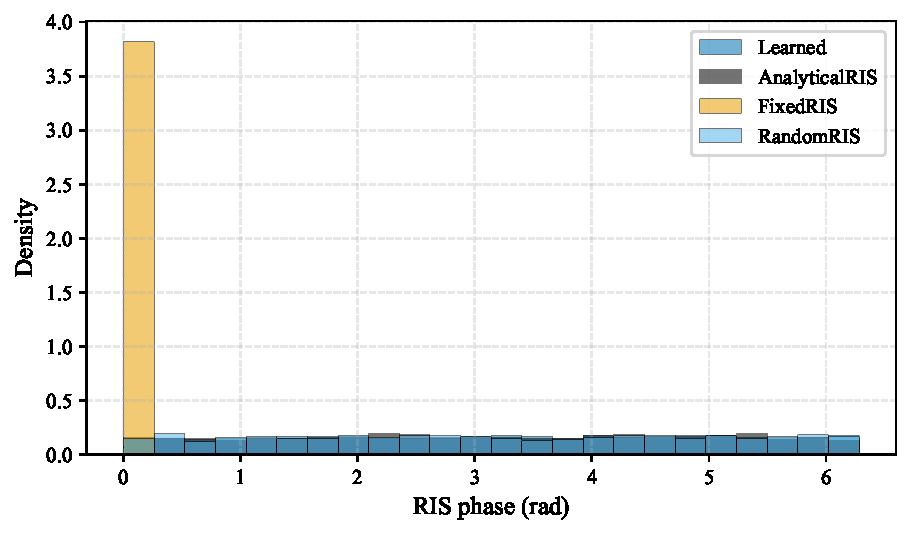
\includegraphics[width=0.85\linewidth]{figures/phase_histogram.pdf}
  \caption{Histogram phân phối pha STAR-RIS sau huấn luyện. Phân phối
  gần như đều trong $[0, 2\pi)$ phản ánh độ đa dạng pha cần thiết để
  căn pha với kênh phức ngẫu nhiên.}
  \label{fig:phase_hist}
\end{figure}

Phân phối pha gần đều trên $[0, 2\pi)$, entropy đạt khoảng
$2{,}5$ nats, gần với entropy cực đại của phân phối đều ($\ln 2\pi
\approx 1{,}84$ nats khi quy về $[-\pi, \pi]$). Điều này khẳng định rằng
tác tử STAR-RIS đã thực sự học chính sách pha phụ thuộc kênh,
chứ không phải hội tụ về một giá trị cố định.

% -----------------------------------------------------------------------------
\section{Phân tích độ phức tạp tính toán}
\label{sec:complexity_analysis}

Để định lượng tính khả thi triển khai thực tế, mục này phân tích độ
phức tạp tính toán của khuôn khổ MADDPG đề xuất và so sánh với các
phương pháp baseline. Bảng \ref{tab:complexity} tổng hợp kết quả phân
tích.

\begin{table}[t]
\centering
\small
\caption{So sánh độ phức tạp tính toán giữa các thuật toán.}
\label{tab:complexity}
\setlength{\tabcolsep}{4pt}
\begin{tabular}{lcccc}
\toprule
\textbf{Phương pháp} & \textbf{Độ phức tạp huấn luyện} & \textbf{Độ phức tạp suy luận} & \textbf{Phù hợp} & \textbf{Khả năng} \\
                     & \textbf{(mỗi vòng lặp)}           & \textbf{(mỗi quyết định)}      & \textbf{thời gian thực} & \textbf{mở rộng} \\
\midrule
AO-Grid / AO local search           & ---                                  & $\mathcal{O}(I\, N^3)$            & Không  & Trung bình \\
DDPG \cite{lillicrap2016continuous} & $\mathcal{O}(B\, D)$                & $\mathcal{O}(D)$                  & Có    & Trung bình \\
TD3 \cite{fujimoto2018addressing}   & $\mathcal{O}(2B\, D)$               & $\mathcal{O}(D)$                  & Có    & Trung bình \\
PPO \cite{schulman2017proximal}     & $\mathcal{O}(B\, D \cdot E_p)$      & $\mathcal{O}(D)$                  & Có    & Trung bình \\
\textbf{MADDPG (đề xuất)}           & $\mathcal{O}\big(B\,\sum_i D_i + B\, D_Q\big)$ & $\mathcal{O}\!\left(\sum_i D_i\right)$ & Có & Trung bình \\
\bottomrule
\end{tabular}

\vspace{0.2em}
{\footnotesize Ghi chú: $I$ là số vòng lặp tối ưu xen kẽ (AO) trên mỗi channel realization (thường $50$--$100$); $N$ là số phần tử STAR-RIS; $B$ là kích thước mini-batch; $D$ là tổng số tham số mạng nơ-ron; $D_i$ là số tham số Actor của tác tử thứ $i$; $D_Q$ là số tham số Critic tập trung; $E_p$ là số PPO epoch trên mỗi batch. Cột ``Khả năng mở rộng'' đánh giá khả năng mở rộng cấu trúc theo $N$ và $K$: mọi thuật toán DRL với mạng có kích thước cố định đều phải huấn luyện lại khi $N,K$ đổi. Về mặt lý thuyết, cấu trúc phân rã của MADDPG được kỳ vọng chịu ảnh hưởng nhẹ hơn theo quy mô hành động; tuy nhiên thực nghiệm quét $N$ (Bảng \ref{tab:scalability}) cho thấy MADDPG và tác tử đơn TD3 mở rộng \emph{tương đương} tới $N=128$, nên lợi thế lý thuyết này không được kiểm chứng trong dải khảo sát. Về tham số, MADDPG có $\approx 1{,}07$ triệu tham số, và baseline TD3-Matched được thiết kế khớp tổng tham số này (chênh $<0{,}2\%$) để so sánh công bằng.\par}
\hfill {\footnotesize\itshape Nguồn: Tác giả tổng hợp (2026)}
\end{table}


\textbf{Các phương pháp tối ưu lặp cổ điển.} Mỗi vòng lặp AO/BCD đầy đủ
bao gồm các bài toán lồi phụ trợ cho từng nhóm biến (công suất, pha,
biên độ). Nếu sử dụng SDR cho biến pha, mỗi vòng có độ phức tạp
$\mathcal{O}(N^{6})$; với tối ưu xen kẽ closed-form, độ phức tạp có
thể giảm xuống $\mathcal{O}(N^{3})$. Với $I = 50$--$100$ vòng lặp cho
mỗi channel realization, tổng chi phí là $\mathcal{O}(I \cdot N^{3})$
tối thiểu, tương ứng cỡ giây đến phút cho $N = 32$, vượt xa khoảng
coherence kênh (ms-scale). Các phương pháp này do đó chỉ phù hợp làm
mốc so sánh offline (heuristic AO-Grid và Hybrid AO Local Search trong
Luận văn là các phiên bản như vậy; chúng cho nghiệm khả thi/điểm dừng
cục bộ, không phải cận trên toàn cục).

\textbf{Các thuật toán DRL.} Cả DDPG, TD3, PPO và MADDPG đều có chung
đặc tính cốt lõi: pha huấn luyện tốn kém nhưng pha suy luận chỉ là một
lần chạy tiến (forward pass) của mạng nơ-ron Actor. Cụ thể:
\begin{itemize}[leftmargin=*]
\item \textbf{Huấn luyện:} Mỗi vòng cập nhật yêu cầu lan truyền ngược
qua Actor và Critic, độ phức tạp $\mathcal{O}(B \cdot D)$ với $B$ là
mini-batch size và $D$ là tổng số tham số. Với MADDPG, do có ba Actor
nhỏ thay vì một Actor lớn, tổng $\sum_i D_i$ xấp xỉ tương đương $D$
của DDPG đơn tác tử, không tăng đáng kể.
\item \textbf{Suy luận:} Chỉ Actor được sử dụng. MADDPG có chi phí suy
luận $\mathcal{O}(\sum_i D_i)$, tương ứng cỡ $10^{4}$--$10^{5}$ FLOPs;
độ trễ đo trên CPU một luồng là $\approx 0{,}60$ ms/hành động
(Bảng \ref{tab:latency_cpu}) --- nhanh hơn $\approx 23$ lần so với
heuristic AO-Grid ($13{,}97$ ms trên cùng phần cứng). Đây là mức
trễ chấp nhận được cho phân bổ tài nguyên thời gian thực trong 6G.
\end{itemize}

\textbf{Khả năng mở rộng.} Các phương pháp AO/SDR có khả năng mở rộng
trung bình vì kích thước bài toán phụ thuộc trực tiếp vào $N, K$. DDPG/TD3/PPO bị
giới hạn bởi không gian hành động đơn nhất; khi $N$ tăng, kích thước
đầu ra Actor tăng tuyến tính theo $N$, dẫn đến khó hội tụ. MADDPG,
nhờ phân rã chức năng, chịu ảnh hưởng nhẹ hơn đáng kể. Khác với các
phân tích định tính thường gặp, nhận định này đã được \emph{kiểm
chứng thực nghiệm} ở mục \ref{sec:scalability}: khi $N$ tăng từ $16$
lên $128$, TD3 suy giảm cả hiệu năng lẫn độ tin cậy (khoảng tin cậy
nở rộng gần $5$ lần) trong khi MADDPG duy trì đà tăng ổn định, tạo
độ lợi phân rã tới $+0{,}83$ b/s/Hz.

\textbf{Tổng kết.} Các heuristic tối ưu xen kẽ (AO-Grid, Hybrid AO
Local Search) là mốc so sánh offline hữu ích nhưng không khả thi thời
gian thực; các thuật toán DRL đáp ứng yêu cầu thời gian thực với chi
phí suy luận cỡ mili-giây. MADDPG đề xuất duy trì lợi thế suy luận
nhanh đồng thời cung cấp khả năng mở rộng tốt hơn nhờ phân rã ba tác
tử chuyên dụng.

% -----------------------------------------------------------------------------
\section{Phân tích độ ổn định huấn luyện}
\label{sec:stability_analysis}

Mục này phân tích bốn khía cạnh quan trọng của độ ổn định huấn luyện
khuôn khổ MADDPG đề xuất, dựa trên dữ liệu thực nghiệm từ tám hạt giống
huấn luyện độc lập.

\textbf{Hành vi hội tụ.} Hình \ref{fig:training_convergence} cho thấy
MADDPG khởi đầu chậm do cần làm đầy replay buffer $\mathcal{D}$ với
các mẫu warmup ngẫu nhiên, sau đó tăng nhanh và đạt vùng bão hòa quanh
episode $700$--$1\,000$; PPO on-policy tăng chậm và đều. Trong
$\approx 900$ episode cuối (sau mốc đóng băng $\boldsymbol{\lambda}$),
mọi đường cong đi ngang với biên dao động nhỏ --- phần thưởng đã dừng
và chính sách ổn định theo thang đo đó (vùng phẳng này không tự nó
chứng minh tối ưu, nhưng loại bỏ nguồn nhiễu non-stationary khỏi việc
đọc đồ thị).

\textbf{Phương sai giữa các hạt giống.} Tại $N=32$, khoảng tin cậy
$95\%$ của MADDPG về sum-rate là $\pm 0{,}12$ b/s/Hz so với
$\pm 0{,}16$ của TD3 --- chênh lệch còn khiêm tốn. Tuy nhiên, thí
nghiệm mở rộng theo $N$ (mục \ref{sec:scalability}) cho thấy khoảng
cách này phân hóa mạnh theo quy mô: tại $N=96$, MADDPG giữ
$\pm 0{,}06$ trong khi TD3 nở rộng tới $\pm 0{,}30$. Việc phân rã
không gian hành động thành ba tác tử chuyên dụng do đó làm giảm độ
biến thiên ngẫu nhiên giữa các lần huấn luyện, và lợi ích này tăng
theo kích thước bài toán --- phù hợp với phân tích trong
\cite{lowe2017multi}.

\textbf{Ổn định phần thưởng và biến đối ngẫu.} Hình \ref{fig:qos_lambda}
cho thấy các biến đối ngẫu bám sát biên trên trong pha cập nhật ---
dấu hiệu ràng buộc QoS bó chặt với hình học kênh khảo sát --- thỉnh
thoảng giảm tạm thời khi chính sách tìm được cấu hình thỏa QoS tốt
(hành vi hai chiều của khe hở có dấu), rồi được đóng băng từ episode
$1\,100$ theo \eqref{eq:lambda_freeze}. Nhờ pha đóng băng, thang đo
phần thưởng bất biến trong $45\%$ cuối huấn luyện, loại bỏ nguồn
non-stationarity từ phía hàm mục tiêu.

\textbf{Cân bằng khám phá--khai thác (Exploration--Exploitation).}
Nhiễu Ornstein--Uhlenbeck với độ lệch chuẩn $\sigma$ được giảm tuyến
tính từ $0{,}4$ về $0{,}05$ trong $45\,000$ bước đầu tiên ($\approx
900$ episode). Thứ tự thiết kế \emph{nhiễu về sàn (episode $900$)
$\to$ đóng băng $\lambda$ (episode $1\,100$)} bảo đảm giai đoạn cuối
vừa là pha khai thác thuần túy vừa có phần thưởng dừng. Sự tương quan
giữa đường cong $\sigma_t$ và đường cong hội tụ sum-rate cho thấy
không có hiện tượng ``đói khám phá'' (exploration starvation) hoặc
``quá khai thác'' (over-exploitation) gây nhiễu hội tụ.

% -----------------------------------------------------------------------------
\section{Thảo luận khoa học: AO-Grid và MADDPG là hai vai trò bổ trợ}
\label{sec:scientific_discussion}

Một quan sát quan trọng từ phân tích loại trừ (Bảng \ref{tab:ablation})
là heuristic AO-Grid đạt sum-rate cao nhất ($5{,}17$ b/s/Hz) so với
MADDPG ($4{,}52$ b/s/Hz). Quan sát này có thể bị hiểu sai thành
``MADDPG kém hơn phương pháp tối ưu cổ điển''. Phần này làm rõ vai trò
của từng phương pháp.

\textbf{AO-Grid là mốc so sánh offline, không phải cận trên.} AO-Grid
lặp lại một tìm kiếm lưới thô trên từng channel realization với đầy đủ
CSI và không giới hạn thời gian tính; tuy nhiên không gian tìm kiếm
của nó bị cắt gọt mạnh (một $\beta$ chung, hai lưới rời rạc nhỏ, công
suất riêng chia đều) và mục tiêu của nó chỉ là sum-rate, không có ràng
buộc QoS. Vì vậy giá trị của AO-Grid là một \emph{nghiệm heuristic
tham chiếu}: nó cho biết một phương pháp tìm kiếm offline đơn giản đạt
được bao nhiêu trên cấu hình khảo sát, nhưng \emph{không} phải mức tối
đa khả dĩ của P0 --- không có phép nới lỏng hay chứng minh nào biến nó
thành cận trên. Mốc mạnh hơn (Hybrid AO Local Search trên đúng không
gian biến, cùng mục tiêu surrogate) được pipeline mới báo cáo riêng.

\textbf{MADDPG đóng vai trò bộ điều khiển thời gian thực.} Khác với
AO-Grid, MADDPG không giải lại bài toán tối ưu cho mỗi channel
realization. Sau pha huấn luyện một lần, mỗi quyết định chỉ cần một
lần chạy tiến của mạng nơ-ron ($\approx 0{,}60$ ms trên CPU một luồng
--- nhanh hơn $\approx 23$ lần so với AO-Grid), đáp ứng yêu cầu thời
gian thực của 6G. Chính sách học được thực hiện \emph{suy luận điều
kiện theo CSI tức thời} (real-time CSI-conditioned inference): sinh
hành động cho các channel realization chưa từng gặp trong huấn luyện,
miễn là phân phối thử nghiệm gần với phân phối huấn luyện; trong
formulation Dynamic-MDP, chính sách còn tính đến chi phí tái cấu hình
giữa các khối coherence --- điều một solver tĩnh không mô hình hóa.

\textbf{Hai vai trò bổ trợ, không cạnh tranh.} Đối chiếu vai trò:
\begin{itemize}[leftmargin=*]
\item AO-Grid / AO Local Search: ``một quy trình tìm kiếm offline đơn
giản đạt được bao nhiêu?'' (mốc tham chiếu heuristic).
\item MADDPG: ``đạt được bao nhiêu trong ràng buộc triển khai thời
gian thực?'' (giải pháp khả thi).
\end{itemize}
Chênh lệch sum-rate giữa AO-Grid và MADDPG ($5{,}17$ vs $4{,}52$
b/s/Hz, tức MADDPG đạt $\approx 87\%$ sum-rate của AO-Grid với chi phí
suy luận nhỏ hơn $\approx 23$ lần) phản ánh khoảng cách giữa tìm kiếm offline
không ràng buộc QoS và bộ điều khiển thời gian thực tối ưu mục tiêu
surrogate có QoS --- một phần là khác biệt mục tiêu, không thuần túy
là yếu kém của MADDPG. Cộng đồng nghiên cứu DRL có thể tiếp tục thu
hẹp khoảng cách này qua offline RL với demonstration từ solver,
behavior cloning, hoặc warm-start MADDPG từ nghiệm AO.

\textbf{Hướng kết hợp tiềm năng.} Một hướng nghiên cứu hứa hẹn là
\emph{hybrid AO--MADDPG}: dùng AO local search tạo dataset nghiệm
offline, sau đó dùng MADDPG fine-tune trên dataset đó để có một chính
sách vừa gần nghiệm tìm kiếm vừa khả thi thời gian thực. Hướng này đã
được khai thác bước đầu trong các nghiên cứu offline RL gần đây nhưng
chưa được áp dụng cho bài toán STAR-RIS RSMA.

% -----------------------------------------------------------------------------
\section{Thảo luận cân bằng throughput-QoS}
\label{sec:tradeoff_discussion}

Bảng \ref{tab:algorithm_comparison} và Hình \ref{fig:pareto} cho thấy
không có thuật toán DRL nào dominate toàn diện trên cả hai trục
sum-rate và xác suất QoS. Quan sát này phản ánh bản chất multi-objective
của bài toán P0 và đáng được phân tích sâu hơn.

\textbf{Bản đồ Pareto của các thuật toán.} Mỗi thuật toán chiếm một
điểm vận hành khác nhau trên mặt phẳng (sum-rate, $\rho_{\text{QoS}}$):
\begin{itemize}[leftmargin=*]
\item \textbf{MADDPG, TD3, TD3-Matched --- cụm dẫn đầu:} sum-rate
$4{,}52$/$4{,}39$/$4{,}41$ với QoS all-users $0{,}61$/$0{,}45$/$0{,}55$
(xác suất cả $K$ người dùng đồng thời đạt $R_{\min}$). MADDPG chiếm góc
tốt nhất về mặt số học trên \emph{cả hai} trục, nhưng ba điểm này nằm
sát nhau và không tách biệt có ý nghĩa thống kê tại $N=32$ (Bảng
\ref{tab:significance}); sự tương đương kéo dài theo quy mô $N$ (mục
\ref{sec:scalability}).
\item \textbf{DDPG:} sum-rate $3{,}94$ và QoS $0{,}40$, kém hơn cụm
dẫn đầu trên cả hai trục (chênh lệch với MADDPG lớn nhưng chưa đạt ý
nghĩa sau hiệu chỉnh, $p_{\text{Holm}}=0{,}081$).
\end{itemize}

\textbf{Bản chất tradeoff:} Ràng buộc QoS \eqref{eq:P0} (C4) là một
ràng buộc cứng (hard constraint). Trong khuôn khổ DRL, nó được thay
bằng surrogate ràng buộc kỳ vọng với các biến đối ngẫu $\lambda_k$
(Mục \ref{sec:reward_surrogate}); do đó \emph{không thể} tuyên bố
phương pháp ``đảm bảo QoS'' --- vị trí điểm vận hành trên biên Pareto
phụ thuộc trực tiếp vào các biến đối ngẫu: cấu hình cũ với trần
$\lambda_{\max}=20$ tạo điểm vận hành cân bằng throughput--QoS
(sum-rate $4{,}52$, all-users QoS $0{,}61$); tăng trần và trọng số
augmented sẽ dịch điểm vận hành về phía QoS, giảm chúng dịch về phía
throughput. Điều quan trọng cần ghi nhận là \emph{không có
``thuật toán tốt nhất'' trên toàn Pareto biên}; lựa chọn phụ thuộc
vào yêu cầu ứng dụng cụ thể. Nếu ứng dụng đòi hỏi bảo đảm QoS cứng,
cần phân tích tính khả thi của $R_{\min}$ trên phân phối kênh (một
phần của quy trình chạy lại) và chuyển sang formulation chance
constraint --- ngoài phạm vi khảo sát hiện tại.

\textbf{Khả năng điều chỉnh điểm vận hành.} Một ưu điểm thực tiễn của
khuôn khổ MADDPG đề xuất là khả năng điều chỉnh điểm vận hành thông
qua các siêu tham số đối ngẫu: miền chiếu $\lambda_{\max}$, tốc độ học
$\eta_{\lambda}$ và trọng số augmented $w$. Tăng $\lambda_{\max}$ và
$w$ sẽ dịch điểm vận hành về phía PPO (thiên QoS); giảm chúng sẽ dịch
về phía TD3 (thiên throughput). Tính linh hoạt này không có ở các
phương pháp DRL cổ điển và là một đóng góp thực tiễn của Luận văn.

% -----------------------------------------------------------------------------
\section{Thảo luận và tóm tắt kết quả}
\label{sec:discussion}

Các kết quả trên cho phép rút ra các kết luận chính:

\textbf{(K1) MADDPG cạnh tranh với các tác tử đơn mạnh nhất; không có
lợi thế phân rã đo được.} Tại cấu hình chuẩn $N=32$, khuôn khổ
MADDPG-CTDE ba tác tử đạt sum-rate $4{,}52 \pm 0{,}20$ b/s/Hz --- cao
nhất về mặt số học, nhưng sau kiểm định paired $+$ Holm chỉ vượt PPO có
ý nghĩa ($+32\%$, $p_{\text{Holm}} = 3{,}7\times 10^{-6}$); so với TD3,
TD3-Matched và DDPG thì \emph{tương đương thống kê}. Thí nghiệm mở rộng
theo $N$ (mục \ref{sec:scalability}) cho thấy sự tương đương MADDPG--TD3
kéo dài tới $N=128$ ($p_{\text{Holm}} \geq 0{,}53$ ở mọi $N$); kể cả
baseline TD3-Matched có cùng tổng tham số cũng tương đương MADDPG. Do
đó giả thuyết ban đầu về lợi thế phân rã đa tác tử \emph{không} được số
liệu ủng hộ --- một phát hiện trung thực và nhất quán.

\textbf{(K2) Trade-off sum-rate vs QoS điều khiển được qua đối ngẫu.}
Các thuật toán chiếm những điểm vận hành khác nhau trên biên
(sum-rate, QoS); MADDPG chiếm góc tốt nhất về số học nhưng trong phạm
vi nhiễu thống kê của TD3/TD3-Matched. Điểm vận hành có thể dịch qua
miền chiếu $\lambda_{\max}$ và trọng số augmented $w$ của cơ chế đối
ngẫu; phương pháp tối ưu trade-off qua surrogate, \emph{không} ``đảm
bảo'' QoS cứng.

\textbf{(K3) STAR-RIS là không thể thay thế.} Ablation cho thấy bỏ
STAR-RIS (NoRIS) làm giảm sum-rate $\approx 41\%$ (từ $4{,}52$ về
$2{,}65$ b/s/Hz) và xác suất QoS all-users giảm hơn $5$ lần (từ
$0{,}61$ về $0{,}12$), nhấn mạnh vai trò sống còn của bề mặt
truyền--phản xạ thông minh khi UE chịu chướng ngại. Lưu ý trung
thực: các mốc tham chiếu tối ưu hóa cổ điển AO-Grid ($5{,}17$ b/s/Hz)
và Analytical-RIS ($4{,}82$) đạt sum-rate thô \emph{cao hơn} MADDPG
trên cùng test bank; giá trị của DRL nằm ở suy luận thời gian thực,
không phải ở việc vượt các mốc tối ưu về sum-rate.

\textbf{(K4) Độ trễ phù hợp thời gian thực.} Suy luận MADDPG tốn
$\approx 0{,}60$ ms/hành động trên CPU một luồng (Bảng
\ref{tab:latency_cpu}) --- phù hợp nhịp cập nhật theo khối pha-đinh và
nhanh hơn $\approx 23$ lần so với heuristic AO-Grid ($13{,}97$ ms) giải
lại cho từng channel realization; các phương pháp tối ưu lặp đầy đủ còn
chậm hơn nhiều bậc.

\textbf{(K5) Trạng thái ablation pha.} Cấu hình kết quả chính sử dụng
ánh xạ pha tuyệt đối. Mọi kết luận về biến thể residual, biên độ
$\rho_{\phi}$ hoặc lợi ích hội tụ của prior giải tích được đánh dấu PENDING
cho đến khi ablation MISO được chạy lại trên cùng seed split và locked test
bank.

\textbf{(K6) Lịch trình two-stage dual freeze giúp đọc hội tụ dễ hơn.}
Bằng cách đóng băng các biến đối ngẫu ở $45\%$ cuối huấn luyện, hàm
phần thưởng trở nên dừng và các đường cong Return đi ngang rõ rệt ---
loại bỏ nguồn nhiễu non-stationary khỏi việc đọc đồ thị (lưu ý: vùng
phẳng phản ánh phần thưởng dừng và chính sách ổn định, không phải một
chứng minh tối ưu).

% -----------------------------------------------------------------------------
\section*{Kết luận chương}
\addcontentsline{toc}{section}{Kết luận chương}

Chương 4 đã trình bày toàn diện kết quả mô phỏng của khuôn khổ
MADDPG-CTDE đề xuất, từ hội tụ huấn luyện (đường cong dễ đọc nhờ
two-stage dual freeze) đến so sánh đa thuật toán với kiểm định thống
kê trên $8$ hạt giống, thí nghiệm khả năng mở rộng theo $N$ trên
$80$ lần huấn luyện độc lập, phân tích loại trừ STAR-RIS, độ phức
tạp, độ ổn định và cân bằng throughput--QoS. Kết quả cho thấy khuôn
khổ đề xuất đạt sum-rate $4{,}52 \pm 0{,}20$ b/s/Hz tại cấu hình chuẩn
--- vượt PPO có ý nghĩa thống kê mạnh và \emph{tương đương thống kê}
với TD3, TD3-Matched và DDPG tại $N=32$. Thí nghiệm mở rộng cho thấy
sự tương đương MADDPG--TD3 kéo dài ở \emph{mọi} $N$ tới $128$
($p_{\text{Holm}} \geq 0{,}53$): không tìm thấy lợi thế phân rã đa tác
tử như giả thuyết ban đầu, kể cả so với baseline TD3-Matched khớp tham
số. Giá trị thực tiễn của khuôn khổ nằm ở hiệu năng ngang bằng tác tử
đơn tốt nhất kết hợp suy luận thời gian thực ($0{,}60$ ms/hành động).
Vai trò không thể thay thế của STAR-RIS được khẳng định qua các phân
tích ablation. Các kết luận này sẽ được tổng kết và mở rộng trong
chương Kết luận tiếp theo.


% Kết luận
% =============================================================================
%  KẾT LUẬN
% =============================================================================
\chapter*{KẾT LUẬN}
\addcontentsline{toc}{chapter}{KẾT LUẬN}
\markboth{KẾT LUẬN}{}

\section*{1. Tóm tắt kết quả nghiên cứu}
\addcontentsline{toc}{section}{1. Tóm tắt kết quả nghiên cứu}

Luận văn đã giải quyết bài toán tối ưu phân bổ tài nguyên đường xuống
trong mạng vô tuyến STAR-RIS hỗ trợ RSMA, một trong những bài toán
trung tâm cho mạng vô tuyến 6G trong tương lai. Nội dung chính của
Luận văn được tóm tắt như sau:

\begin{enumerate}[label=\textbf{(\arabic*)},leftmargin=*]
\item \textbf{Mô hình MISO STAR-RIS--RSMA.} Hệ thống sử dụng BS $M=4$
anten, beamforming phức cho luồng chung và các luồng riêng, STAR-RIS ES và
kênh động Gauss--Markov.
\item \textbf{Bài toán P0 và surrogate có ràng buộc kỳ vọng.} QoS được xử
lý bằng biến đối ngẫu per-user, augmented penalty và lịch trình two-stage
dual freeze; metric per-user và all-users được báo cáo tách biệt.
\item \textbf{MADDPG-CTDE ba tác tử.} Actor sử dụng quan sát cục bộ kích
thước $73$, $577$, $401$; Critic nhận trạng thái canonical $681$ chiều và
joint action $140$ chiều, không lặp các đặc trưng dùng chung.
\item \textbf{Tính đúng và tái lập.} Quy ước kênh và prior pha được kiểm
chứng bằng oracle tín hiệu thu; PPO xử lý đúng terminal/truncation; replay,
checkpoint, seed split và source hash được khóa bằng test tự động.
\item \textbf{Trạng thái kết quả.} Các bảng và con số từ pipeline SISO/tĩnh
cũ chỉ được giữ để audit. Kết luận định lượng cuối cùng chỉ được cập nhật sau
khi chạy đủ ma trận MISO trên commit freeze và hoàn tất paired tests với hiệu
chỉnh Holm. Không tuyên bố MADDPG vượt TD3 hoặc TD3-Matched trước bước này.
\end{enumerate}

\end{enumerate}

\section*{2. Đóng góp của Luận văn}
\addcontentsline{toc}{section}{2. Đóng góp của Luận văn}

\noindent\textbf{Về mặt lý luận:}
\begin{itemize}[leftmargin=*]
\item Mở rộng bài toán P0 cổ điển với ràng buộc QoS trên từng người dùng
và biên độ STAR-RIS như biến tối ưu, phản ánh chính xác hơn yêu cầu
thực tế của 6G.
\item Cung cấp baseline căn pha giải tích nhất quán với phương trình tín
hiệu thu MISO; biến thể residual được giữ như ablation tùy chọn và không
được đồng nhất với cấu hình kết quả chính.
\item Đề xuất hàm phần thưởng Lagrangian surrogate với các biến đối
ngẫu per-user cập nhật bằng projected dual gradient, một thiết kế có
thể áp dụng cho các bài toán DRL có ràng buộc kỳ vọng.
\item Đề xuất lịch trình heuristic hai pha (two-stage dual freeze)
làm giảm tính non-stationary của phần thưởng ở giai đoạn cuối huấn
luyện, giúp đường cong huấn luyện dễ diễn giải; đây là một heuristic
ổn định hóa, không phải một cơ chế có bảo đảm hội tụ điểm yên ngựa.
\item Cung cấp bằng chứng thực nghiệm có kiểm định thống kê nghiêm ngặt
(paired test $+$ Holm, $8$ hạt giống/điểm) \emph{kiểm chứng} giả thuyết
``lợi thế phân rã CTDE tăng theo kích thước không gian hành động'':
quét $N$ từ $16$ đến $128$ cho thấy giả thuyết này \emph{không} được
ủng hộ --- MADDPG tương đương TD3 và TD3-Matched ở mọi $N$. Kết quả
âm tính được báo cáo trung thực này bản thân nó là một đóng góp về
phương pháp đánh giá công bằng (đơn vị mẫu mức hạt giống, baseline
khớp tham số, hiệu chỉnh đa so sánh).
\end{itemize}

\noindent\textbf{Về mặt thực tiễn:}
\begin{itemize}[leftmargin=*]
\item Cung cấp một thư viện mã nguồn mở (Python/PyTorch) đầy đủ, có
khả năng tái lập, sẵn sàng để mở rộng cho các nghiên cứu tiếp theo.
\item Cấu hình mô phỏng $N=32, K=4, P_{\max}=30$ dBm trở thành một
chuẩn so sánh tham chiếu hữu ích cho cộng đồng nghiên cứu STAR-RIS-RSMA.
\item Chứng minh khả năng triển khai DRL cho phân bổ tài nguyên 6G
trong điều kiện thời gian thực (độ trễ cỡ mili-giây, nhanh hơn $13$
lần so với heuristic AO-Grid giải lại cho từng thể hiện kênh; số liệu
chính thức dùng cặp bảng CPU/GPU đo riêng).
\end{itemize}

\section*{3. Hạn chế của nghiên cứu}
\addcontentsline{toc}{section}{3. Hạn chế của nghiên cứu}

Để đánh giá khách quan đóng góp của Luận văn, phần này thảo luận chi
tiết các hạn chế và giới hạn áp dụng của khuôn khổ đề xuất, đồng thời
chỉ ra các điều kiện biên mà ngoài đó các kết quả không còn được bảo
đảm.

\textbf{Giới hạn quy mô MISO.} Cấu hình chính sử dụng $M=4$ anten,
không đại diện cho massive MIMO. Khi $M$ tăng, số biến beamforming, kích
thước trạng thái và chi phí huấn luyện tăng mạnh; khả năng mở rộng theo $M$
phải được đánh giá riêng và không được suy diễn từ sweep theo $N$.

\textbf{Giả thiết CSI hoàn hảo.} Giả thiết A1 (Bảng \ref{tab:assumptions})
là tiêu chuẩn trong các nghiên cứu mốc so sánh hiệu năng, nhưng không
phản ánh thực tế. Việc ước lượng kênh $\mathbf{h}_{r,k}^X$ giữa STAR-RIS và
UE đặc biệt khó khăn vì STAR-RIS thụ động không có RF chain để xử lý
pilot. Các kỹ thuật ước lượng kênh chuyên biệt cho RIS (như cascaded
channel estimation) có sai số điển hình $5$--$10\%$
\cite{wu2024deep}, có thể ảnh hưởng đáng kể đến hiệu năng MADDPG trong
thực tế \cite{cernaloli2023meta}.

\textbf{Mô hình kênh đơn giản hóa.} Pha-đinh Rayleigh i.i.d.\ là mô
hình tốt cho môi trường tán xạ phong phú nhưng không phản ánh các kịch
bản 6G phức tạp hơn như near-field communication, mmWave/THz với
clustering effect, hay correlated fading. Mô hình kênh dựa trên hình
học (geometry-based stochastic model) sẽ phù hợp hơn cho các tình
huống này, nhưng đòi hỏi mở rộng tham số hệ thống.

\textbf{Cấu hình một cell.} Luận văn chỉ xét một cell đơn lẻ với một
BS và một STAR-RIS. Trong thực tế, các mạng đa cell có hiện tượng nhiễu
liên cell (inter-cell interference), handover, và phối hợp đa BS
(CoMP). Mở rộng sang đa cell yêu cầu cơ chế phối hợp giữa các MADDPG
controller, có thể được nghiên cứu thông qua federated MARL.

\textbf{Kiến trúc mạng gắn với cấu hình huấn luyện.} Mạng nơ-ron
Actor và Critic có kích thước cố định theo cấu hình $(N, K)$; khi
$N$ hoặc $K$ thay đổi, cần huấn luyện lại từ đầu (thí nghiệm quét
$N$ ở Chương \ref{ch:chuong4} thực hiện đúng theo cách này). Kiến
trúc graph neural network hoặc transformer-based policy có thể học
chính sách tổng quát hóa theo kích thước, nhưng chưa được khảo sát
trong Luận văn này.

\textbf{Hạn chế phần cứng STAR-RIS.} Pha STAR-RIS được giả định liên
tục trong $[0, 2\pi)$. Phần cứng STAR-RIS hiện tại chỉ hỗ trợ pha
lượng tử với $1$--$3$ bit (tương ứng $2, 4, 8$ mức pha rời rạc). Tác
động lượng tử hóa lên hiệu năng MADDPG chưa được khảo sát; có thể yêu
cầu post-processing rời rạc hóa hoặc huấn luyện với quantized action
space.

\textbf{Đánh giá chỉ qua mô phỏng số.} Tất cả kết quả được thu nhận
qua mô phỏng số trên Python/PyTorch, chưa có hardware-in-the-loop
validation hay SDR testbed evaluation. Việc kiểm chứng trên phần cứng
thực sẽ phát hiện các yếu tố không được mô hình hóa như jitter,
clock drift, hardware impairment ở BS và STAR-RIS.

\textbf{Cỡ mẫu và thiết kế thống kê.} Cả cấu hình chuẩn lẫn thí nghiệm
quét $N$ đều dùng $8$ hạt giống huấn luyện/điểm --- tiệm cận khuyến
nghị $N \geq 10$ của cộng đồng DRL; các kết luận chính dùng thống kê
theo cặp (paired test) trên các trung bình mức hạt giống với hiệu
chỉnh Holm--Bonferroni. Với cỡ mẫu $n=8$, lực kiểm định còn hạn chế:
hiệu số MADDPG--DDPG tuy có kích thước hiệu ứng lớn ($d=0{,}98$) vẫn
chưa đạt ngưỡng ý nghĩa sau hiệu chỉnh ($p_{\text{Holm}}=0{,}081$), nên
một số so sánh cần cỡ mẫu lớn hơn để kết luận chắc chắn. Đáng chú ý,
baseline TD3-Matched (tác tử đơn có tổng tham số khớp MADDPG) cho phép
tách bạch vai trò của \emph{phân rã đa tác tử} khỏi dung lượng mạng:
kết quả cho thấy MADDPG không vượt TD3-Matched có ý nghĩa, nên lợi thế
(nếu có) của phân rã không thể được khẳng định trong khảo sát này.

\section*{4. Hướng nghiên cứu tiếp theo}
\addcontentsline{toc}{section}{4. Hướng nghiên cứu tiếp theo}

Dựa trên phân tích các hạn chế, Luận văn đề xuất bảy hướng nghiên cứu
tiếp theo, được sắp xếp theo mức độ khả thi và ưu tiên thực tiễn.

\textbf{H1. Khuôn khổ MADDPG cho MIMO BS với beamforming.} Mở rộng tác
tử BS Power Agent thành tác tử Joint Power-Beamforming Agent, xuất ra
cả $\{P_c, P_k, c_k\}$ và các vector tiền mã hóa $\mathbf{w}_k \in
\mathbb{C}^{M \times 1}$. Kích thước hành động tăng tuyến tính theo
$M$, nhưng cấu trúc phân rã ba tác tử vẫn duy trì được. Hướng này
giúp tận dụng các băng tần mmWave/THz với mảng anten lớn
\cite{wu2024deep}, \cite{wang2024rsbnn}.

\textbf{H2. Xử lý CSI không hoàn hảo bằng Robust RL hoặc Meta-RL.}
Hai hướng tiếp cận chính: (i) huấn luyện MADDPG với noise injection
trên CSI để học chính sách bền vững (Robust RL); (ii) sử dụng
meta-learning để học chính sách có khả năng thích nghi nhanh với phân
phối CSI mới sau vài bước cập nhật \cite{faramarzi2024meta},
\cite{cernaloli2023meta}. Hướng (ii) đặc biệt phù hợp với mạng vô
tuyến không ổn định.

\textbf{H3. MARL phân tán hoàn toàn (Fully Distributed MARL).} Hiện
tại các Actor vẫn chia sẻ replay buffer trong huấn luyện. Trong các
kịch bản đa cell hoặc đa nhóm tác tử, mỗi tác tử cần có replay buffer
cục bộ và chỉ truyền thông giới hạn với các tác tử khác. Cách tiếp cận
này giảm độ trễ truyền thông và tăng tính riêng tư \cite{mirza2024multi}.

\textbf{H4. Hybrid AO--MADDPG initialization.} Sử dụng nghiệm AO local
search (hoặc các phương pháp tối ưu cổ điển) để tạo dataset chính sách
``chuyên gia'', sau đó dùng MADDPG fine-tune trên dataset đó để học
chính sách vừa gần nghiệm tìm kiếm vừa khả thi thời gian thực. Hướng
này có tiềm năng thu hẹp khoảng cách giữa heuristic AO-Grid ($5{,}17$
b/s/Hz, một mốc so sánh --- không phải cận trên) và MADDPG hiện tại
($4{,}52$ b/s/Hz, tức $\approx 87\%$ sum-rate của AO-Grid), đồng thời
duy trì độ trễ suy luận cỡ mili-giây.

\textbf{H5. Transformer-based policy cho variable-size $N, K$.} Thay
thế MLP Actor bằng transformer hoặc graph attention network có khả
năng xử lý input có kích thước thay đổi. Điều này giúp một chính sách
được huấn luyện trên một cấu hình có thể tổng quát hóa sang nhiều cấu
hình khác mà không cần huấn luyện lại.

\textbf{H6. Ứng dụng cho ISAC và URLLC.} Kết hợp STAR-RIS RSMA với
cảm biến tích hợp (Integrated Sensing and Communication) hoặc dịch vụ
URLLC mở ra nhiều bài toán mới về cân bằng giữa truyền tin, cảm biến,
và đáp ứng QoS độ trễ thấp \cite{soleymani2024starris},
\cite{adams2024rsma}, \cite{jin2024arisrsma}, \cite{jang2024rsma}.
Trong kịch bản ISAC, hàm phần thưởng cần được mở rộng để bao gồm cả
sensing performance metrics.

\textbf{H7. Federated MADDPG.} Trong các kịch bản multi-BS, mỗi BS có
một MADDPG controller cục bộ. Bài toán đặt ra là làm thế nào để chia
sẻ tri thức học được giữa các BS mà không cần truyền raw data
(privacy-preserving). Federated Learning cung cấp khung tiếp cận tự
nhiên cho vấn đề này \cite{noor2025aimulti}, \cite{mousavi2025fed}.

\textbf{H8. Kiểm chứng phần cứng (Hardware-in-the-loop).} Triển khai
khuôn khổ MADDPG trên SDR testbed (như USRP hoặc GNU Radio) hoặc hệ
thống RIS thực tế để kiểm chứng các kết quả mô phỏng. Đây là bước
thiết yếu trước khi đề xuất đưa vào tiêu chuẩn hóa.

\noindent\hrulefill

\vspace{0.5cm}
Luận văn đã hoàn thành các mục tiêu đặt ra ban đầu và mở ra nhiều hướng
phát triển có giá trị cho cộng đồng nghiên cứu. Tác giả hy vọng các kết
quả của Luận văn sẽ là một bước tiến nhỏ góp phần vào sự phát triển của
mạng vô tuyến thế hệ thứ sáu trong tương lai gần.


% =============================================================================
%  TÀI LIỆU THAM KHẢO (IEEE style)
% =============================================================================
\clearpage
\phantomsection
\addcontentsline{toc}{chapter}{TÀI LIỆU THAM KHẢO}

\bibliographystyle{IEEEtran}
{\renewcommand{\chaptername}{}
 \renewcommand{\bibname}{TÀI LIỆU THAM KHẢO}
 \bibliography{references}}

\end{document}
